
\documentclass[thmcnt=section, color=blue, 12pt]{my-elegantbook}

\usepackage{bbm}

% Index page
\usepackage{imakeidx}
\makeindex[columns=2, intoc, options=-s index_style.ist]

% Title and author
\title{Mathematical Analysis}
\author{Isaac FEI}

% Reference file
\addbibresource{mathematical-analysis.bib} 

% Image of the book cover
\cover{cover.png}

\begin{document}

% Print title and cover page
\maketitle

%--------
% Preface
%--------

\frontmatter
\chapter*{Preface}

This book mainly follows the structure of \cite{apostolMathematicalAnalysisModern1974}.

%------------------------------

% Print table of contents
\tableofcontents
\mainmatter

%-------------------------------
% Main document starts from here
%-------------------------------

%==============================

\chapter{Point-Set Topology}

%==============================

\chapter{Functions of Bounded Variation and Rectifiable Curves}

%------------------------------ 

\section{Functions of Bounded Variation}

\begin{definition}
	Let $[a, b]$ be an interval.
	A set of points
	\begin{align*}
		P = \{ x_0, x_1, \dots, x_n \}
	\end{align*}
	satisfying
	\begin{align*}
		a = x_0 < x_1 < \cdots < x_n = b
	\end{align*}
	is called a \textbf{partition}\index{partition of an interval} of $[a, b]$.

	The interval $[x_{k-1}, x_k]$ is called the $k$-th subinterval of $P$,
	and we often write $\Delta x_k = x_k - x_{k-1}$.

	The collection of all partitions of $[a, b]$ is denoted by $\CALP [a, b]$.
\end{definition}


\begin{note}
	In mathematics texts, we have another definition of partitions,
	which states that a partition of a set $S$ is a collection of subsets of $S$
	such that they are disjoint and their union equals $S$.
	We should not confuse these two definitions.
\end{note}

\begin{definition}
	Let $f$ be a real-valued function on $[a, b]$.
	If $P = \{x_0, \dots x_n\}$ is a partition of $[a, b]$,
	write $\Delta f_k = f(x_k) - f(x_{k-1})$.
	If there exists a positive number $M$ such that
	\begin{align}
		\sum_{k=1}^n \abs{\Delta f_k} \leq M \label{eq:1}
	\end{align}
	for all partitions $P$ of $[a, b]$, then we say that $f$
	is \textbf{of bounded variation}\index{functions of bounded variation}
	on $[a, b]$.
\end{definition}

\begin{note}
	A geometric interpretation of the sum $\sum_{k=1}^n \abs{\Delta f_k}$
	is the total vertical length of several pieces of the function.
	Imagine a point moving along the curve of the function from the
	left to the right.
	If the partition gets finer and finer,
	then $\sum_{k=1}^n \abs{\Delta f_k}$
	will become the length of its journey projected on the $y$-axis.
	In fact, it is defined as the total variation as we shall introduce later.
\end{note}

Sometimes, it is convenient to denote the sum $\sum_{k=1}^n \abs{\Delta f_k}$
by the symbol
\begin{align*}
	v(P, f) := \sum_{k=1}^n \abs{\Delta f_k}
\end{align*}
We do not use the capital letter $V$ here for it is reserved for
the total variation.

A simple observation is that a function of bounded variation is also bounded.

\begin{proposition} \label{prop:2}
	Let $f$ be a function of bounded variation on $[a, b]$.
	Then $f$ is bounded on $[a, b]$.
\end{proposition}

\begin{proof}
	By definition, there exists $M > 0$ such that \eqref{eq:1} holds
	for any partitions of $[a, b]$.
	For any $x \in (a, b)$, consider the partition $P = \{a, x, b\}$.
	We have
	\begin{align*}
		\abs{f(x) - f(a)} + \abs{f(b) - f(x)} \leq M
	\end{align*}
	This implies that $\abs{f(x) - f(a)} \leq M$, which further
	implies $\abs{f(x)} \leq \abs{f(a)} + M$.
	Note that $x$ is arbitrarily chosen from $(a, b)$.
	Therefore, $f$ is indeed bounded on $[a, b]$.
\end{proof}

But a bounded function is not necessarily of bounded variation.

\begin{example} \label{eg:1}
	Consider the function
	\begin{align*}
		f(x) = \begin{cases}
			       \cos \frac{1}{x}, & x \in (0, 1] \\
			       0,                & x = 0
		       \end{cases}
	\end{align*}
	Its graph is shown in Figure~\ref{fig:1}.
	\begin{figure}[H]
		\centering
		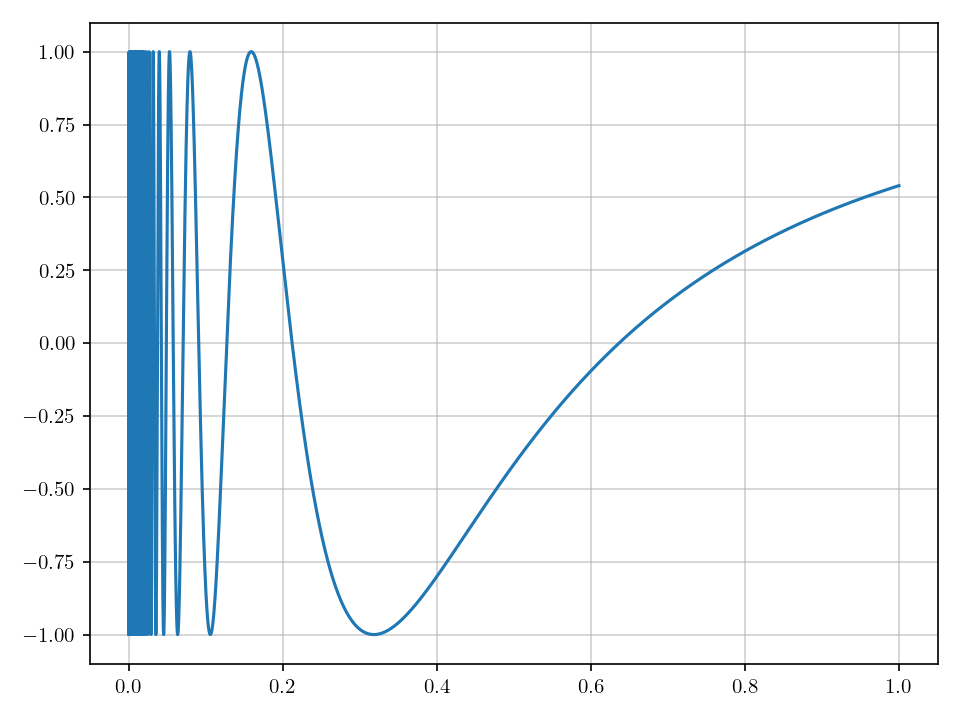
\includegraphics[width=0.7\textwidth]{figures/bounded-function-that-is-not-of-bounded-variation.png}
		\caption{Graph of the function $f(x) = \cos\frac{1}{x}$ for $x \in (0, 1]$ and $f(0) = 0$. It is bounded on $[0, 1]$ but not of bounded variation for it varies rapidly near $x=0$.}
		\label{fig:1}
	\end{figure}
	Clearly, this function is bounded by $1$.
	But intuitively, it is not of bounded variation since it varies rapidly
	near $x=0$.
	Let $P$ be a partition of $[0, 1]$ where each $x_k$ is given by
	\begin{align*}
		x_k = \begin{cases}
			      \frac{1}{(n-k) \pi}, & 1 \leq k \leq n-1 \\
			      0,                   & k = 0             \\
			      1,                   & k = n
		      \end{cases}
	\end{align*}
	For $k=1, \dots, n-1$, we have
	\begin{align*}
		f(x_k) = \cos ( (n-k) \pi ) \in \{-1, 1\}
	\end{align*}
	The function value is either $1$ or $-1$ and the sign alternates between
	each two consecutive points. Hence,
	\begin{align*}
		\sum_{k=1}^{n} \abs{\Delta f_k}
		\geq \sum_{k=2}^{n-1} \abs{\Delta f_k} = 2 (n - 2)
	\end{align*}
	As we increase the number of points in the partition, $\sum \abs{\Delta f_k}$
	will exceeds any given number.
	Therefore, $f$ is not of bounded variation on $[0, 1]$.
\end{example}

\begin{proposition} \label{prop:1}
	If $f$ is monotonic on $[a, b]$, then $f$ is of bounded variation on $[a, b]$.
\end{proposition}

\begin{proof}
	Assume $f$ is increasing.
	For any partition $P = \{x_0, \dots, x_n\}$ of $[a, b]$, we have
	\begin{align*}
		\sum_{k=1}^n \abs{\Delta f_k}
		= \sum_{k=1}^n (f(x_k) - f(x_{k-1}))
		= f(b) - f(a)
	\end{align*}
	Therefore, $f$ is of bounded variation on $[a, b]$.

	If $f$ is decreasing, then $-f$ is increasing.
	Applying what we have proved, we may conclude that $-f$ is of bounded variation.
	Hence, $f$ is also of bounded variation
	since $\sum \abs{\Delta (-f)_k} = \sum \abs{\Delta f_k}$.
\end{proof}

\begin{proposition} \label{prop:3}
	Suppose that $f$ is continuous on $[a, b]$ and the
	derivative $f^\prime$ exists in $(a, b)$.
	If $\abs{f^\prime(x)} \leq A$ for all $x \in (a, b)$,
	then $f$ is of bounded variation on $[a, b]$.
\end{proposition}

\begin{note}
	The assumption that $f$ being continuous on $[a, b]$,
	and $f^\prime$ exists in $(a, b)$ coincides with the mean value theorem.
	And indeed, it is the key of this proof.
\end{note}

\begin{proof}
	Let $P = \{x_0, \dots, x_n\}$ be a partition of $[a, b]$.
	By the mean value theorem, there exists $t_k \in (x_{k-1}, x_k)$
	for all $k=1, \dots, n$ such that
	\begin{align*}
		f(x_k) - f(x_{k-1}) = f^\prime(t_k) (x_k - x_{k-1})
	\end{align*}
	It then follows that
	\begin{align*}
		\sum_{k=1}^n \abs{\Delta f_k}
		 & = \sum_{k=1}^n \abs{f^\prime(t_k)} (x_k - x_{k-1}) \\
		 & \leq \sum_{k=1}^n A (x_k - x_{k-1})                \\
		 & = A (f(b) - f(a))
	\end{align*}
	Therefore, $f$ is of bounded variation on $[a, b]$.
\end{proof}

The following is a well crafted example of showing that
a continuous and differentiable function is not necessarily
of bounded variation
if we do not impose that its derivative is bounded in the interior.

\begin{example}
	Consider function defined on $[0, 1]$ given by
	\begin{align*}
		f(x) = \begin{cases}
			       x \cos \frac{\pi}{2x}, & x \in (0, 1] \\
			       0,                     & x = 0
		       \end{cases}
	\end{align*}
	Its graph is shown in Figure \ref{fig:2}.

	\begin{figure}[H]
		\centering
		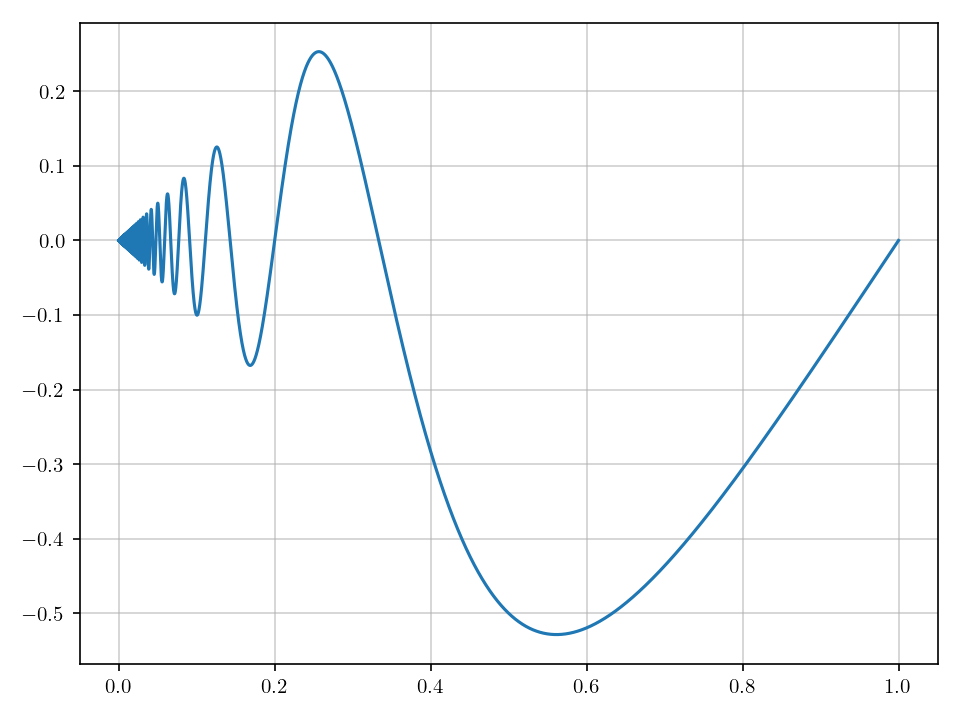
\includegraphics[width=0.7\textwidth]{figures/continuous-function-that-is-not-of-bounded-variation.png}
		\caption{Graph of the function $f(x) = x \cos \frac{\pi}{2x}$ for $x \in (0, 1]$ and $f(0) = 0$. This function is continuous and its derivative exists in $(0, 1)$. But the derivative is unbounded.}
		\label{fig:2}
	\end{figure}

	The fact that this function is not of bounded variation may be less intuitive
	than the one given in Example~\ref{eg:1}.
	The function still varies rapidly near $x=0$.
	However, it does not range from $-1$ and $1$.
	Instead, it damps out at $x=0$ and becomes $0$.
	But we will show in the following that we can find a partition so fine that
	by collecting each small function variation,
	the overall sum may still increase to infinity.

	Consider the partition
	\begin{align*}
		P = \{0, \frac{1}{2n}, \frac{1}{2n - 1}, \dots, \frac{1}{3}, \frac{1}{2}, 1\}
	\end{align*}
	We have
	\begin{align*}
		\sum_k \abs{\Delta f_k}
		 & = \frac{1}{2n} + \frac{1}{2n} + \frac{1}{2n - 1} + \frac{1}{2n - 1}
		+ \dots + \frac{1}{2} + \frac{1}{2}                                    \\
		 & = 1 + \cdots + \frac{1}{n}
	\end{align*}
	As $n$ gets larger and larger,
	the sum on the right hand-side will increase infinitely
	for we know that the harmonic series $\sum \frac{1}{n}$ diverges.
	Therefore, this function is not of bounded variation.
\end{example}

Of course, the condition of the derivative being bounded is not necessary
for a function to be of bounded variation.

\begin{example}
	The derivative of the square root function $f(x) = \sqrt{x}$ in $(0, 1)$
	is $f^\prime(x) = \frac{1}{2\sqrt{x}}$,
	which tends to infinity as $x \to 0$.
	But $f$ is clearly of bounded variation on $[0, 1]$
	by Proposition~\ref{prop:1} for it is increasing.
\end{example}

Let $P$ be a partition of $[a, b]$.
If we make it finer by adding some intermediate points,
then the sum of variations will increase.
This result may be helpful in some proofs.

\begin{proposition} \label{prop:4}
	Let $f$ be defined on $[a, b]$,
	and $P$ a partition of $[a, b]$.
	If $P^\prime$ is finer than $P$, i.e., $P^\prime \supset P$,
	then
	\begin{align*}
		v(P^\prime, f) \geq v(P, f)
	\end{align*}
\end{proposition}

\begin{note}
	Compare this to the upper and lower Darboux sums
	when we introduce them in a later section.
\end{note}

\begin{proof}
	It suffices to that prove for the case
	where $P^\prime$ is one point finer than $P$.
	Suppose $P = \{x_0, \dots, x_n\}$ and $P^\prime = P \sqcup \{c\}$.
	We have
	\begin{align*}
		v(P^\prime, f)
		 & = \abs{f(x_1) - f(x_0)} + \cdots
		+ \abs{f(c) - f(x_{j-1})} + \abs{f(x_j) - f(c)} + \cdots
		+ \abs{f(x_n) - f(x_{n-1})}            \\
		 & \geq \abs{f(x_1) - f(x_0)} + \cdots
		+ \abs{f(x_j) - f(x_{j-1})} + \cdots
		+ \abs{f(x_n) - f(x_{n-1})}            \\
		 & = v(P, f)
	\end{align*}
	\begin{note}
		Note that $j$ may equal to $1$ or $n$ in the above notations.
		We write down the summation in the expanded form
		to make the proof easier to read.
	\end{note}
	This completes the proof.
\end{proof}

%------------------------------ 

\section{Total Variation}

Recall that $f$ is said to be of bounded of variation
on $[a, b]$ if, equivalently to what we stated, the set
\begin{align}
	\set{\sum_{k=1}^n \abs{\Delta f_k}}{P \in \CALP [a, b]}
	\label{eq:2}
\end{align}
or with our shortened notation
\begin{align*}
	\set{v(P, f)}{P \in \CALP[a, b]}
\end{align*}
is bounded above.
This set is of course nonempty for $\{a, b\}$ is clearly a partition.
By the least upper bound property,
the set in \eqref{eq:2} has a supremum, which is referred to as
\textbf{total variation}\index{total variation} of $f$ on $[a, b]$.

\begin{definition}
	Let $f$ be of bounded variation on $[a, b]$.
	The total variation, denoted by $V_a^b (f)$,
	of $f$ on $[a, b]$ is defined as
	\begin{align*}
		V_a^b (f)
		:= \sup_{P \in \CALP [a, b]} v(P, f)
		= \sup \set{\sum_{k=1}^n \abs{\Delta f_k}}{P \in \CALP [a, b]}
	\end{align*}
\end{definition}

\begin{note}
	We adopt the notation $V_a^b(f)$,
	which is inspired by the notion of
	a definite integral $\int_a^b f(x) \dif x$.
	And as we shall see,
	these two concepts indeed share some similar properties, namely,
	the linear properties.

	Notations are very important for they provide intuitive expressions
	of the intrinsic mathematical concepts.
\end{note}

From this definition,
we have some simple observations.
First, the value of $V_a^b (f)$ is nonnegative.
And it is easy to prove that $V_a^b (f) = 0$
if and only if $f$ is constant on $[a, b]$.

The simplest function of bounded variation
(well, apart from a constant function) is
monotonic function.
It is natural to ask what is its total variation.
With a little thought,
one can imagine that
it should be the absolute value of the difference at the endpoints.

\begin{proposition}
	If $f$ is a monotonic function on $[a, b]$,
	then its total variation is the absolute value of the difference
	of the function values at the endpoints, i.e.,
	\begin{align*}
		V_a^b(f) = \abs{f(a) - f(b)}
	\end{align*}
\end{proposition}

\begin{proof}
	We only prove the case that $f$ is increasing.
	For any partition $P = \{x_0, \dots, x_n\}$ of $[a, b]$, we have
	\begin{align*}
		\sum_{k=1}^n \abs{f(x_k) - f(x_{k-1})}
		= \sum_{k=1}^n [f(x_k) - f(x_{k-1})]
		= f(b) - f(a)
	\end{align*}
	Note that the sum is independent of the partition.
	Hence, the set in \eqref{eq:2} is just a constant.
	Therefore, the total variation $V_a^b(f) = f(b) - f(a)$.
\end{proof}

When studying functions of bounded variation,
in most cases, we are often interested in
monotonic functions
or continuous and differentiable functions.
(Proposition~\ref{prop:1} and \ref{prop:3}.)

\begin{note}
	On one hand, we will see in Theorem~\ref{thm:4},
	a function is of bounded variation if and only if
	it can be expressed as a difference
	of two increasing functions,
	the need of studying monotonic functions arises naturally.

	On the other hand, as we shall see in the chapter on Riemann-Stieltjes integrals,
	we assume the integrator $\alpha$ is of bounded variation.
	Since integrator $\alpha$ will be put after the
	differential operator, $\dif \alpha$,
	and we often hope to express it as $\alpha^\prime(t) \dif t$
	to reduce the integral to Riemann integral
	and compute its value,
	we would like $\alpha$ to be differentiable.
\end{note}

But if we are curious about whether some piecewise functions
are of bounded variation,
then Proposition~\ref{prop:1} and \ref{prop:3} will not be enough.

\begin{example} \label{eg:2}
	For example, consider the following function defined on $[0, 3]$:
	\begin{align*}
		f(x) = \begin{cases}
			       x,           & 0 \leq x \leq 1 \\
			       -(x-1)(x-3), & 1 < x \leq 3
		       \end{cases}
	\end{align*}
	Figure~\ref{fig:4} depicts its graph.
	\begin{figure}[H]
		\centering
		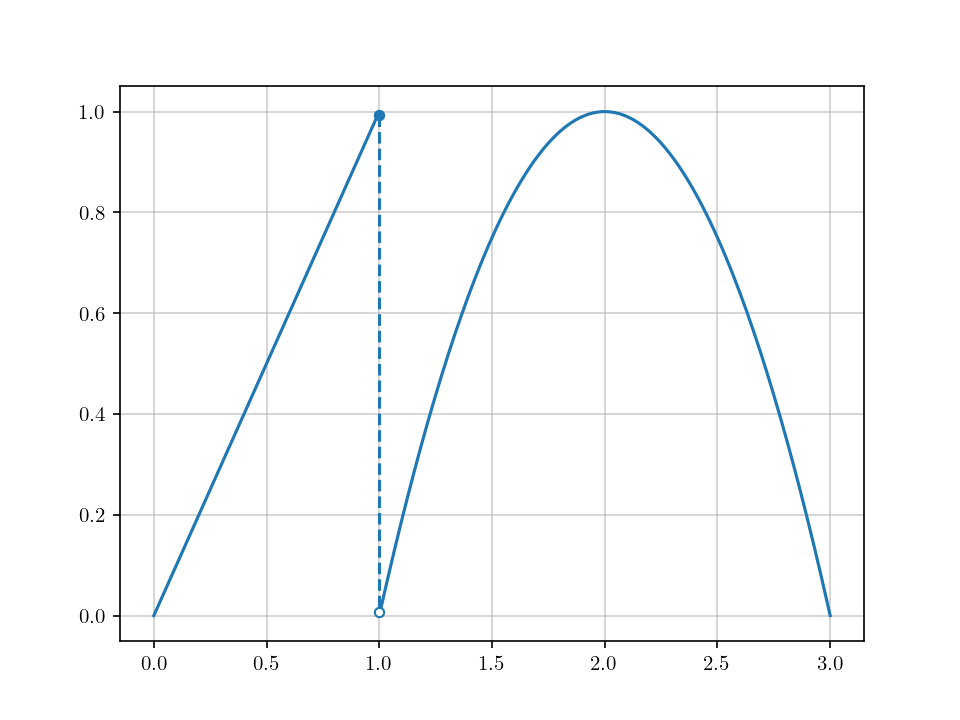
\includegraphics[width=0.7\textwidth]{figures/piecewise-function-of-bounded-variation.png}
		\caption{Is this function of bounded variation on $[0, 3]$?}
		\label{fig:4}
	\end{figure}

	Intuitively, the function in Figure~\ref{fig:4} should be of bounded variation.
	But we must be careful about the jump point,
	which we have not covered in the previous discussion.
\end{example}

\begin{proposition} \label{prop:5}
	Suppose $f$ is of bounded variation on $[a, b]$,
	and is continuous at $x = a$.
	If function $g$ is defined by revising the value at $x=a$, i.e.,
	\begin{align*}
		g(x) = \begin{cases}
			       f(x), & x \in (a, b] \\
			       y,    & x = a
		       \end{cases}
	\end{align*}
	then $g$ is still of bounded variation on $[a, b]$.
	And its total variation is given by
	\begin{align*}
		V_a^b(g) = V_a^b(f) + \abs{y - f(a)}
	\end{align*}
\end{proposition}

\begin{proof}
	Let $P$ be a partition of $[a, b]$.
	We have
	\begin{align}
		v(P, g) & = \abs{g(x_1) - g(a)} + \cdots \abs{g(x_n) - g(x_{n-1})}                                     \nonumber \\
		        & = \abs{f(x_1) - y} + \cdots \abs{f(x_n) - f(x_{n-1})}                                       \nonumber  \\
		        & \leq \left[ \abs{y -  f(a)} + \abs{f(x_1) - f(a)} \right] + \cdots \abs{f(x_n) - f(x_{n-1})} \nonumber \\
		        & = \abs{y - f(a)} + v(P, f)                                                                  \nonumber  \\
		        & \leq \abs{y - f(a)} + V_a^b(f)
		\label{eq:12}
	\end{align}
	This shows that $g$ is of bounded variation on $[a, b]$.

	Now, we compute its total variation.
	Let $\varepsilon > 0$ be arbitrary.
	Because $f$ is continuous at $x=a$,
	there exists $\delta > 0$ such that
	\begin{align*}
		\abs{x - a} < \delta \implies \abs{f(x) - f(a)} < \varepsilon/4
	\end{align*}
	By the definition of total variation and Proposition~\ref{prop:4},
	there exists a fine enough partition $P$
	such that the minimum length of the subinterval is less than $\delta$, and
	\begin{align*}
		v(P, f) > V_a^b(f) - \varepsilon/2
	\end{align*}
	On the subinterval $[a=x_0, x_1]$, we have
	\begin{align*}
		\abs{\Delta g_1} & = \abs{g(x_1) - g(x_0)}                                                                     \\
		                 & = \abs{f(x_1) - y}                                                                          \\
		                 & \geq \abs{f(a) - y} - \abs{f(x_1) - f(a)}                                                   \\
		                 & = \abs{f(a) - y} + \abs{f(x_1) - f(a)} -
		2\abs{f(x_1) - f(a)}                                                                                           \\
		                 & \text{Note that $\abs{x_1 - x_0} < \delta$, hence we may estimate the last term as follows} \\
		                 & > \abs{f(a) - y} + \abs{f(x_1) - f(a)} - 2 \cdot \varepsilon/4                              \\
		                 & > \abs{f(a) - y} + \abs{f(x_1) - f(a)} - \varepsilon/2
	\end{align*}
	\begin{note}
		When reaching
		\begin{align*}
			\abs{\Delta g_1} \geq \abs{f(a) - y} - \abs{f(x_1) - f(a)}
		\end{align*}
		in the above derivation,
		one may be worried that
		it is not proceeding towards the goal
		since we have a minus sign before $\abs{f(x_1) - f(a)}$.
		But since this term $\abs{f(x_1) - f(a)}$ can be made arbitrarily small,
		we can always add it (to construct the sum $v(P, f)$)
		and then subtract it,
		and make the trailing negative term $-2\abs{f(x_1) - f(a)}$ negligible,
		as what we did above.
	\end{note}
	It then follows that
	\begin{align*}
		v(P, g) > \abs{f(a) - y} + v(P, f) - \varepsilon/2
		> \abs{f(a) - y} + V_a^b(f) - \varepsilon
	\end{align*}
	Therefore, we have
	\begin{align*}
		V_a^b(g) \geq v(P, g) \geq \abs{f(a) - y} + V_a^b(f)
	\end{align*}
	Compare this to \eqref{eq:12}, we may conclude
	\begin{align*}
		V_a^b(g) = V_a^b(f) + \abs{f(a) - y}
	\end{align*}

\end{proof}

The function $f$ in Example~\ref{eg:2} can be regarded as a sum
of two functions on $[0, 3]$, $f(x) = g(x) + h(x)$ where
\begin{align*}
	g(x) & = \begin{cases}
		         x, & x \in [0, 1] \\
		         0, & x \in (1, 3]
	         \end{cases}            &  & = (x \mapsto x) \ind_{[0, 1]} \\
	h(x) & = \begin{cases}
		         0,            & x \in [0, 1) \\
		         \tilde{h}(x), & x \in [1, 3]
	         \end{cases} &  & = \tilde{h} \ind_{[1, 3]}
\end{align*}
where
\begin{align*}
	\tilde{h}(x) = \begin{cases}
		               -(x-1)(x-3), & x \in (1, 3] \\
		               0,           & x = 1
	               \end{cases}
\end{align*}

We have already seen that functions like $\tilde{h}$ are of bounded variation
in Proposition~\ref{prop:5}.
If we know the sum of two functions of bounded variation (on the same interval)
is also of bounded variation (Theorem~\ref{thm:1}),
we may then conclude that piecewise functions like $f$ in Example~\ref{eg:2}
are indeed of bounded variation.

Hence, the next step to do is studying
whether functions like $g$ and $h$ are of bounded variation.
Describing in words,
such functions are constructed
by extending a function of bounded variation
to a larger interval by defining function values of everywhere else
in the larger interval to be zeros.



\begin{theorem} \label{thm:1}
	Let $f$ and $g$ be of bounded variation on $[a, b]$, then
	so are their sum, difference and product.
	Moreover, we have the following inequalities:
	\begin{align}
		V_a^b (f \pm g)  \leq V_a^b (f) + V_a^b (g)
		\label{eq:3}
	\end{align}
	and
	\begin{align}
		V_a^b (fg)       \leq \sup_{x \in [a, b]} \abs{g(x)} V_a^b (f)
		+ \sup_{x \in [a, b]} \abs{f(x)} V_a^b (g)
		\label{eq:4}
	\end{align}
\end{theorem}

\begin{note}
	Note that the supremums in \eqref{eq:4} indeed exist
	since the functions $f$ and $g$ are bounded due to Proposition~\ref{prop:2}.
\end{note}

\begin{proof}
	We first show that the sum and the difference of two functions
	are of bounded variation, and satisfy \eqref{eq:3}.
	Let $P$ be an arbitrary partition of $[a, b]$.
	On each subinterval, we have
	\begin{align*}
		\abs{\Delta (f \pm g)_k}
		 & = \abs{f(x_{k}) \pm g(x_{k}) - [f(x_{k-1}) \pm g(x_{k-1})]} \\
		 & = \abs{\Delta f_k \pm \Delta g_k}                           \\
		 & \leq \abs{\Delta f_k} + \abs{\Delta g_k}
	\end{align*}
	Taking the sum over $k$, we have
	\begin{align*}
		\sum_{k} \abs{\Delta (f \pm g)_k}
		\leq \sum_{k} \abs{\Delta f_k} + \sum_k \abs{\Delta g_k}
		\leq V_a^b (f) + V_a^b (g)
	\end{align*}
	The above inequality shows that $f \pm g$ is of bounded variation on $[a, b]$,
	and \eqref{eq:3} is satisfied.

	In the following, we show that the product of two Functions
	are of bounded variation and satisfies \eqref{eq:4}.
	Let $P$ be an arbitrary partition of $[a, b]$.
	On each subinterval, we have
	\begin{align*}
		\abs{\Delta (fg)_k}
		 & = \abs{f(x_{k}) g(x_{k}) - f(x_{k-1}) g(x_{k-1})}                                \\
		 & \text{Add and subtract the term $f(x_{k-1})g(x_{k})$}                            \\
		 & = \abs{ g(x_{k})[ f(x_{k}) - f(x_{k-1})] + f(x_{k-1})[ g(x_{k}) - g(x_{k-1}) ] } \\
		 & \leq \abs{g(x_{k})} \abs{\Delta f_k} + \abs{f(x_{k-1})} \abs{ \Delta g_k }       \\
		 & \leq \sup_{x \in [a, b]} \abs{g(x)} \abs{\Delta f_k}
		+ \sup_{x \in [a, b]} \abs{f(x)} \abs{\Delta g_k}
	\end{align*}
	Summing over $k$, we have
	\begin{align*}
		\sum_k \abs{\Delta (fg)_k}
		\leq \sup_{x \in [a, b]} \abs{g(x)} \sum_k \abs{\Delta f_k}
		+ \sup_{x \in [a, b]} \abs{f(x)} \sum_k \abs{\Delta g_k} \\
		\leq  \sup_{x \in [a, b]} \abs{g(x)} V_a^b (f)
		+ \sup_{x \in [a, b]} \abs{f(x)} V_a^b (g)
	\end{align*}
	This shows the product $fg$ is in fact of bounded variation on $[a, b]$,
	and \eqref{eq:4} is satisfied.
\end{proof}

We must exclude the quotients from the above theorem
since the reciprocal $\frac{1}{f}$ of $f$ may not be of bounded variation
even though $f$ is.

\begin{example}
	Consider function
	\begin{align*}
		f(x) = \begin{cases}
			       1-x, & 0 \leq x < 1     \\
			       -x,  & 1 \leq x  \leq 2
		       \end{cases}
	\end{align*}
	Function $f$ is of bounded variation on $[0, 2]$ since it is decreasing.
	Its reciprocal is
	\begin{align*}
		\frac{1}{f(x)} = \begin{cases}
			                 \frac{1}{1-x}, & 0 \leq x < 1     \\
			                 -\frac{1}{x},  & 1 \leq x  \leq 2
		                 \end{cases}
	\end{align*}
	Figure \ref{fig:3} depicts the graphs of $f$ and $\frac{1}{f}$.
	\begin{figure}[H]
		\centering
		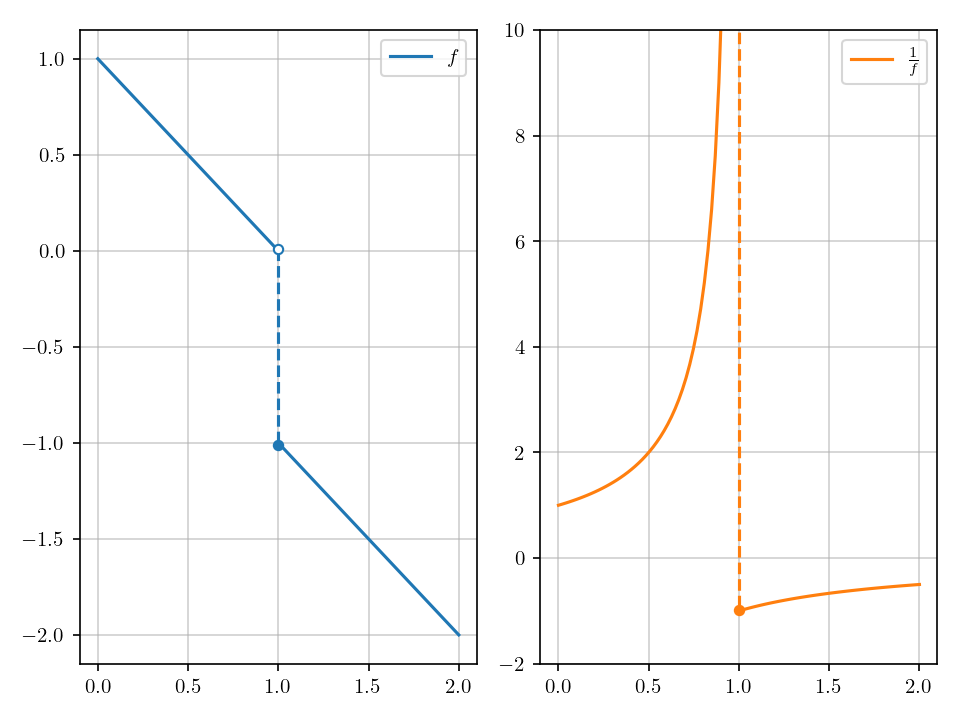
\includegraphics[width=0.7\textwidth]{figures/reciprocal-not-of-bounded-variation.png}
		\caption{Left: $f$ is of bounded variation for it is decreasing. Right: $\frac{1}{f}$ is not of bounded variation for it is unbounded.}
		\label{fig:3}
	\end{figure}
	Note that $\frac{1}{f}$ goes to positive infinity when $x \to 1^-$.
	Therefore, by Proposition~\ref{prop:2}, $\frac{1}{f}$ is not of bounded variation on $[0, 2]$
	since it is not bounded.
\end{example}

To extend Theorem~\ref{thm:1} to quotients,
we need to required that $f$ is bounded away from zero in the interval.

\begin{theorem}
	Let $f$ be of bounded variation on $[a, b]$.
	And there exists $m > 0$ such that $f(x) \geq m$ for all $x \in [a, b]$.
	Then the reciprocal of $f$ is of bounded variation on $[a, b]$, and
	\begin{align*}
		V_a^b ( \frac{1}{f} )
		\leq \frac{1}{m^2} V_a^b (f)
	\end{align*}
\end{theorem}

\begin{proof}
	Let $P$ be any partition of $[a, b]$.
	On each subinterval $[x_{k-1}, x_k]$, we have
	\begin{align*}
		\abs{\Delta (\frac{1}{f})_k}
		 & = \abs{\frac{1}{f(x_k)} - \frac{1}{f(x_{k-1})}} \\
		 & = \abs{\frac{\Delta f_k}{f(x_{k-1}) f(x_k)}}    \\
		 & \leq \frac{\abs{ \Delta f_k }}{m^2}
	\end{align*}
	Summing over $k$, we have
	\begin{align*}
		\sum_k \abs{\Delta (\frac{1}{f})_k}
		\leq \frac{1}{m^2} \sum_k \abs{\Delta f_k}
		\leq \frac{1}{m^2} V_a^b (f)
	\end{align*}
	Therefore, $\frac{1}{f}$ is of bounded variation on $[a, b]$.
\end{proof}

\subsection{Additive Property of Total Variation}

\begin{theorem} \label{thm:2}
	Let $f$ be of bounded variation on $[a, b]$, and $c \in (a, b)$.
	Then $f$ is of bounded variation on the subintervals $[c, b]$ and $[a, c]$.
	Moreover, we have
	\begin{align}
		V_a^b(f) = V_a^c(f) + V_c^b(f)
		\label{eq:9}
	\end{align}
\end{theorem}

\begin{proof}
	We will first show that $f$ is of bounded variation on each subinterval, and
	\begin{align}
		V_a^c(f) + V_c^b(f) \leq V_a^b(f)
		\label{eq:5}
	\end{align}

	Let $P^\prime$ and $P^{\prime\prime}$ be partitions of $[a, c]$ and $[c, b]$,
	respectively,
	and let $P = P^\prime \cup P^{\prime\prime}$.
	Note that $P$ is a partition of $[a, b]$,
	and by reviewing the notation of $v(P, f)$
	one may easily conclude that $v(P^\prime, f) + v(P^{\prime\prime}, f) = v(P, f)$.
	Since $f$ is of bounded of variation on $[a, b]$, we have
	\begin{align}
		v(P^\prime, f) + v(P^{\prime\prime}, f) = v(P, f) \leq V_a^b (f)
		\label{eq:6}
	\end{align}
	The above inequality holds for any partition $p^\prime$ of $[a, c]$
	and any partition $P^{\prime\prime}$ of $[c, b]$.
	Therefore, by definition, $f$ is of bounded variation on $[a, c]$ and $[c, b]$.
	Moreover, taking the supremum over $P^\prime$ and then over $P^{\prime\prime}$
	on both sides of \eqref{eq:6}, we will obtain exactly \eqref{eq:5}.

	To show the equality \eqref{eq:9}, we also need to show
	\begin{align}
		V_a^c(f) + V_c^b(f) \geq V_a^b (f)
		\label{eq:7}
	\end{align}
	Let $\varepsilon > 0$ be arbitrary.
	There exists a partition $P$ of $[a, b]$
	such that $v(P, f) > V_a^b(f) - \varepsilon$.
	Let
	\begin{align*}
		P^\prime = ( P \cap [a, c] ) \cup \{c\} \quad \text{and} \quad
		P^{\prime\prime} = ( P \cap [c, b] ) \cup \{c\}
	\end{align*}
	It is clear that $P^\prime$ and $P^{\prime\prime}$
	are partitions of $[a, c]$ and $[c, b]$, respectively.
	By Proposition~\ref{prop:4}, we have
	\begin{align}
		V_a^c(f) + V_c^b(f) \geq v(P^\prime, f)
		+ v(P^{\prime\prime}, f)
		\geq v(P, f) > V_a^b(f) - \varepsilon
		\label{eq:8}
	\end{align}
	Because \eqref{eq:8} holds for every $\varepsilon > 0$, \eqref{eq:7} is proved.
\end{proof}

Applying the above theorem, we can immediately conclude that $f$
is also of bounded variation on any interval contained in $[a, b]$.

\begin{corollary} \label{cor:1}
	If $f$ is of bounded variation on $[a, b]$,
	and $[c, d] \subseteq [a, b]$,
	then $f$ is also of bounded variation on $[c, d]$.
\end{corollary}

\begin{proof}
	With the given condition, we have $a \leq c < d \leq b$.
	If $c = a$ or $d = b$,
	then the assumption of this corollary reduces to the one in Theorem~\ref{thm:2}.

	Now, we assume that $a < c < d <b$.
	Regarding $c$ as an intermediate point in $[a, b]$,
	Theorem~\ref{thm:2} shows that $f$ is of bounded variation on $[c, b]$.
	Next, because $d \in (c, b)$, applying Theorem~\ref{thm:2} again,
	we conclude that $f$ is of bounded variation on $[c, d]$.
\end{proof}

\subsection{Total Variation as a Function of the Right Endpoint}

Suppose $f$ is of bounded variation on $[a, b]$.
For any $x \in (a, b)$.
Theorem~\ref{thm:2} tells us that $f$ is of bounded variation on $[a, x]$.
Therefore, we can regard $V_a^x (f)$ as a function of $x$.

\begin{note}
	This is very similar to considering $\int_a^x f(t) \dif t$ as a function
	of the upper limit of the integral, which
	again shows that our notation of the total variation rather helpful.
\end{note}

When $x = b$, it is just the total variation of $f$ on the entire interval.
We don't have definition for $x = a$ yet.
But we can easily fix this by naturally defining $V_a^a (f) := 0$.
Now, function $V_a^x(f)$ is defined on the entire interval $[a, b]$.

In the next chapter, we will study the Riemann-Stieltjes integral, which
is more generalized definition of the Riemann integral.
In the texts of the Riemann-Stieltjes integral $\int_a^b f \dif \alpha$,
we often assume that the integrator $\alpha$ is increasing
(or slightly more generalized, monotonic)\cite{rudinPrinciplesMathematicalAnalysis1976}.
But we can extend the results easily to a even more
general assumption that the integrator $\alpha$
is of bounded variation on $[a, b]$.

The key of achieving this is that a function of bounded variation
can be written as a difference of two increasing functions,
and conversely, the difference of two increasing functions
is of bounded variation
(Theorem~\ref{thm:4}).
And the following theorem tells us exactly how to
find such increasing
functions.

\begin{theorem} \label{thm:3}
	Let $f$ be of bounded variation on $[a, b]$.
	Then
	\begin{enumerate}
		\item $V_a^x(f)$ is increasing on $[a, b]$, and
		\item $V_a^x(f) - f(x)$ is also increasing.
	\end{enumerate}
\end{theorem}

\begin{proof}
	Let $h > 0$ (and $x + h \leq b$), by Theorem~\ref{thm:2}, we have
	\begin{align*}
		V_a^x (f) + V_x^{x+h} (f) = V_a^{x+h} (f)
	\end{align*}
	\begin{note}
		We have seen in Corollary~\ref{cor:1} that $V_x^{x+h}(f)$ indeed exists.
	\end{note}
	It then follows that
	\begin{align*}
		V_a^{x+h}(f) - V_a^{x}(f) = V_x^{x+h}(f) \geq 0
	\end{align*}
	This shows $V_a^x(f)$ is increasing.

	Next, we will prove $V_a^x(f) - f(x)$ is creasing.
	To ease the notation, let $g(x) = V_a^x(f) - f(x)$.
	Similarly, suppose $h > 0$ and $x + h \leq b$,
	consider the difference
	\begin{align}
		g(x+h) - g(x)
		= V_x^{x+h}(f) + [f(x+h) - f(x)]
		\label{eq:10}
	\end{align}
	\begin{note}
		Seeing the term $f(x+h) - f(x)$ in the context of total variation,
		we immediately think of the partition $P = \{x, x+h\}$ of $[x, x+h]$.
	\end{note}
	We have
	\begin{align*}
		\abs{f(x+h) - f(x)} \leq V_x^{x+h}(f)
	\end{align*}
	It then follows that
	\begin{align*}
		V_x^{x+h}(f) \geq \abs{f(x+h) - f(x)} \geq -[f(x+h) - f(x)]
	\end{align*}
	which further implies
	\begin{align}
		V_x^{x+h}(f) + [f(x+h) - f(x)] \geq 0
		\label{eq:11}
	\end{align}
	Comparing \eqref{eq:10} and \eqref{eq:11}, we conclude
	that $g(x)$ is indeed increasing.
\end{proof}

\subsection{Characterization of Functions of Bounded Variation}

With the help of Theorem~\ref{thm:3}, we can easily prove
the following elegant theorem,
which characterizes functions of bounded variation.
It states that a function on $[a, b]$ is of bounded variation
if and only if it can be written as a difference of two increasing functions.
The difficult part of find such increasing functions
is already handled by Theorem~\ref{thm:3}.

\begin{theorem} \label{thm:4}
	Let $f$ be defined on $[a, b]$,
	then $f$ is of bounded variation if and only if
	it can be expressed as a difference of two
	increasing functions.
\end{theorem}

\begin{proof}
	We first suppose that $f$ is of bounded variation.
	Then Theorem~\ref{thm:3} shows that $V_a^x(f)$
	and $V_a^x(f) - f(x)$ are both increasing on $[a, b]$.
	Since we can write
	\begin{align*}
		f(x) = V_a^x(f) - [ V_a^x (f) - f(x)]
	\end{align*}
	It is proved.

	Reversely, suppose that $f$ can be expressed as a difference of
	two increasing functions $g$ and $h$ on $[a, b]$, $f = g - h$.
	Proposition~\ref{prop:1} tells us that $g$ and $h$ are of bounded variation
	since they are increasing functions.
	Then by Theorem~\ref{thm:1}, we know that $g - h$ is also of bounded variation.
	This completes the proof.
\end{proof}

\begin{note}
	We can also make these two increasing functions strict.
	Suppose $f = g - h$.
	We can easily achieve this by defining $\tilde{g}(x) = g(x) + x$
	and $\tilde{h}(x) = h(x) + x$.
\end{note}

\section{Continuous Functions of Bounded Variation}

Previously, we have shown that a function $f$ of bounded variation can be
written as the difference of two increasing functions, $f = g - h$.
Now, suppose $f$ is continuous.
We will show in this section that the two increasing functions $g$ and $h$
can also be made continuous as well.

\begin{theorem} \label{thm:24}
	Suppose $f$ is of bounded variation on $[a, b]$.
	Then $f$ is continuous at $x_0 \in [a, b]$
	if and only if $V_a^x(f)$ is continuous at $x_0$.
	In other words, every point of continuity of $f$ is also
	a point of continuity of $V_a^x(f)$ and vice versa.
\end{theorem}

\begin{proof}
	We first suppose that $V_a^x(f)$ is continuous at $x_0$
	and show that $f$ is also continuous at $x_0$,
	which is the easier direction to prove.

	We will only show that $f$ is continuous from the right at $x_0$ ($x_0 \neq b$),
	and the continuity from the left is similarly proved (including $x_0 = b$).
	Let $\varepsilon > 0$ be arbitrary.
	Because $V_a^x(f)$ is continuous at $x_0$,
	there exists $\delta  > 0$ such that
	\begin{align*}
		\abs{x - x_0} < \delta \implies \abs{V_a^x(f) - V_a^x(f)} < \varepsilon
	\end{align*}
	For all $h$ satisfying $0 < h < \delta$, we have
	\begin{align*}
		\abs{f(x_0 + h) - f(x_0)}
		 & = v(P, f) \quad \text{where $P = \{x_0, x_0+h\}$ is a partition of $[x_0, x_0+h]$} \\
		 & \leq V_{x_0}^{x_0+h}(f)                                                            \\
		 & = V_a^{x_0+h}(f) - V_a^{x_0}(f)                                                    \\
		 & < \varepsilon
	\end{align*}
	This shows that $f$ is continuous at $x_0$ from the right.
	Applying a similar argument,
	one may show that it is also continuous at $x_0$ from the left
	by considering the interval $[x_0-h, x_0]$.

	We now prove the reverse direction.
	Suppose $f$ is continuous at $x_0$.
	Again, we will only prove that $V_a^x(f)$
	is continuous at $x_0$ ($x_0 \neq b$) from the right.
	Let $\varepsilon > 0$ be arbitrary.
	Since $f$ is continuous at $x_0$, there exists $\delta > 0$
	such that
	\begin{align*}
		\abs{x-x_0} < \delta \implies \abs{f(x) - f(x_0)} < \varepsilon/2
	\end{align*}
	Consider the total variation $V_{x_0}^b(f)$.
	For any $h$ satisfying $0 < h < \delta$,
	There exists a partition $P$ such that
	\begin{align*}
		x_1 - x_0 \leq \delta
	\end{align*}
	where $x_1 = x_0 + h$
	and
	\begin{align}
		v(P, f) > V_{x_0}^b(f) - \varepsilon/2
		\label{eq:14}
	\end{align}
	\begin{note}
		If one is confusing about how finding such $P$ is possible,
		we can think of finding it with the following process.
		First, find a partition $P$ of $[x_0, b]$ such that
		\begin{align*}
			v(P, f) > V_{x_0}^b(f) - \varepsilon/2
		\end{align*}
		and then refine $P$ to $P^\prime$ by adding a point $c$ in between $x_0$ and $x_1$
		such that $c - x_0 < \delta$.
		Note that $v(P^\prime, f) \geq v(P, f)$ (Proposition~\ref{prop:4}).
		Therefore,
		\begin{align*}
			v(P^\prime, f) > V_{x_0}^b(f) - \varepsilon/2
		\end{align*}
		is satisfied.
		Finally, rename $P^\prime$ to $P$.
	\end{note}
	We can express $v(P, f)$ as
	\begin{align}
		v(P, f)
		 & = \abs{\Delta f_1} + \underbrace{ \abs{\Delta f_2} + \cdots + \abs{\Delta f_n} }_{ \text{$= v(P^\prime, f)$ where $P^\prime$ is a partition of $[x_1, b]$}} \nonumber \\
		 & = \abs{f(x_1) - f(x_0)} + v(P^\prime, f) \nonumber                                                                                                                    \\
		 & \leq \abs{f(x_1) - f(x_0)} + V_{x_1}^b(f) \nonumber                                                                                                                   \\
		 & \text{Recall that $x_1 - x_0 < \delta$ and $f$ is continuous at $x_0$} \nonumber                                                                                      \\
		 & < \varepsilon/2 + V_{x_1}^b(f)
		\label{eq:13}
	\end{align}
	Combining \eqref{eq:14} and \eqref{eq:13}, we obtain
	\begin{align*}
		\varepsilon/2 + V_{x_1}^b(f) > v(P, f) > V_{x_0}^b(f) - \varepsilon/2
	\end{align*}
	Rearranging the terms yields
	\begin{align*}
		\abs{V_a^{x_0+h}(f) - V_a^{x_0}(f)}
		= V_{x_0}^{x_0 + h}(f)
		= V_{x_0}^{x_1}(f)
		= V_{x_0}^b(f) - V_{x_1}^b(f)
		< \varepsilon
	\end{align*}
	(Specially, it also holds for $x_0 = 1$.)
	This shows $V_a^x(f)$ is continuous at $x_0$ from the right.
	And considering $V_a^{x_0}(f)$ and $V_a^{x_0-h}(f)$ and applying a similar argument,
	one can also show that $V_a^{x}(f)$ is continuous at $x_0$ from the left.
\end{proof}

%==============================

\chapter{The Riemann-Stieltjes Integral}

%------------------------------

\section{The Definition of the Riemann-Stieltjes Integral}

\begin{definition} \label{def:1}
	Let $f$ and $\alpha$ be real-valued functions on $[a, b]$.
	Assume $\alpha$ is bounded.
	We say $f$ is
	\textbf{Riemann-Stieltjes integrable}\index{Riemann-Stieltjes integrable}
	with respect to $\alpha$ on $[a, b]$
	if there exists a number $A$ such that
	for any choice of $\varepsilon > 0$,
	we can always find a partition $P_\varepsilon$ of $[a, b]$ such that
	for any partition $P$ finer than $P_\varepsilon$, $P \supseteq P_\varepsilon$,
	and for any list of representatives $T$ of $P$,
	the \textbf{Riemann-Stieltjes sum}\index{Riemann-Stieltjes sum}
	satisfies
	\begin{align*}
		\abs{ S(P, T, f, \alpha) - A } < \varepsilon
	\end{align*}
	The number $A$ is denoted by $\int_a^b f \dif \alpha$
	or more verbose, $\int_a^b f(x) \dif \alpha(x)$,
	and is referred to as the (value of)
	\textbf{Riemann-Stieltjes integral}\index{Riemann-Stieltjes integral}
	(of $f$ w.r.t. $\alpha$ on $[a, b]$).
\end{definition}


In Apostol's definition \cite{apostolMathematicalAnalysisModern1974},
the function $f$ is assumed to be bounded.
This assumption is made because if $f$ is unbounded,
the integral is bound not to exist.
Consequently, Apostol chose not to explore integrals of unbounded functions,
excluding them from his definition.

However, for educational purposes,
we aim to demonstrate explicitly that
the integral does not exist when $f$ is unbounded.
Therefore, we modify the definition to allow $f$
to be unbounded and subsequently prove the non-existence of the integral.

\begin{proposition}
	If $f$ is unbounded, then $f \notin \mathfrak{R}(\alpha)$ on $[a, b]$.
\end{proposition}

\begin{proof}
	We shall prove by contradiction.
	Assume, on the contrary, $f \in \mathfrak{R}(\alpha)$ on $[a, b]$
	and $\int_a^b f \dif \alpha = A$.
	Then there exists a partition $P = \{x_0, \ldots, x_n\}$ of $[a, b]$ such that
	for any list of representatives $T$ of $P$,
	\begin{align}
		\abs{S(P, T, f, \alpha) - A} < \frac{1}{2}
		\label{eq:46}
	\end{align}
	Let $T_0$ be a particular list of representatives.
	Because $f$ is unbounded on $[a, b]$,
	there exists $j \in \{1, \ldots, n\}$
	such that $f$ is unbounded on $[x_{j-1}, x_j]$.
	It then follows that we may choose a
	point $t_j^\prime \in [x_{j-1}, x_j]$
	such that
	\begin{align*}
		\abs{f(t_j^\prime) - f(t_j)} \abs{\Delta \alpha_j} > 1
	\end{align*}
	Let $T^\prime$ be constructed by replacing
	the $j$-th point $t_j$ with $t_j^\prime$ in $T_0$.
	We have
	\begin{align*}
		\abs{S(P, T^\prime, f, \alpha) - S(P, T_0, f, \alpha)}
		= \abs{ [ f(t_j^\prime) - f(t_j) ] \Delta \alpha_j}
		> 1
	\end{align*}
	It then follows that
	\begin{align*}
		\abs{S(P, T^\prime, f, \alpha) - A}
		 & > \abs{S(P, T^\prime, f, \alpha) - S(P, T_0, f, \alpha)}
		- 	\abs{S(P, T_0, f, \alpha) - A}                           \\
		 & > 1 - \frac{1}{2}                                        \\
		 & = \frac{1}{2}
	\end{align*}
	This results in a contradiction with \eqref{eq:46}.
\end{proof}

\section{Linear Properties}

The following theorem shows the linearity of integrals in the fashion of
the integrands.

\begin{theorem}
	If $f, g \in \mathfrak{R}(\alpha)$ on $[a, b]$,
	then $c_1 f + c_2 g \in \mathfrak{R}(\alpha)$ on $[a, b]$.
	And
	\begin{align}
		\int_a^b c_1 f + c_2 g \dif \alpha
		= c_1 \int_a^b f \dif \alpha + c_2 \int_a^b g \dif \alpha
		\label{eq:16}
	\end{align}
\end{theorem}

\begin{proof}
	Let $\varepsilon > 0$ be arbitrary.
	Because $f$ and $g$ are both Riemann integrable on $[a, b]$,
	there exists a partition $P_\varepsilon$ of $[a, b]$
	such that for any $P \supseteq P_\varepsilon$ and
	set of representatives $T$ of $P$ satisfying
	\begin{align}
		\abs{S(P,T,f,\alpha) - \int_a^b f \dif \alpha} < \frac{\varepsilon}{\abs{c_1} + \abs{c_2} + 1}
		\quad \text{and} \quad
		\abs{S(P,T,g,\alpha) - \int_a^b g \dif \alpha} < \frac{\varepsilon}{\abs{c_1} + \abs{c_2} + 1}
		\label{eq:15}
	\end{align}
	\begin{note}
		The reason of the choice of
		the small number $\frac{\varepsilon}{\abs{c_1} + \abs{c_2} + 1}$
		will be clear later.
		And the $+1$ in the denominator is designed for the case that
		both $c_1$ and $c_2$ are zeros.
	\end{note}
	Consider the Riemann-Stieltjes sum $S(P,T,c_1 f + c_2 g, \alpha)$.
	We have
	\begin{alignat*}{2}
		 & \quad &  & \abs{S(P,T,c_1 f + c_2 g, \alpha)
			- c_1 \int_a^b f \dif \alpha
		- c_2 \int_a^b g \dif \alpha}                   \\
		 & =     &  & \abs{
			\sum_k (c_1 \Delta f_k + c_2 \Delta g_k)
			- c_1 \int_a^b f \dif \alpha
		- c_2 \int_a^b g \dif \alpha}                   \\
		 & =     &  & \abs{
			c_1 \sum_k \Delta f_k + c_2  \sum_k \Delta g_k
			- c_1 \int_a^b f \dif \alpha
		- c_2 \int_a^b g \dif \alpha}                   \\
		 & =     &  & \abs{
			c_1 S(P,T,f,\alpha) + c_2 S(P,T,g,\alpha)
			- c_1 \int_a^b f \dif \alpha
		- c_2 \int_a^b g \dif \alpha}                   \\
		 & \leq  &  & \abs{c_1} \abs{
			S(P,T,f,\alpha) - \int_a^b f \dif \alpha
		} + \abs{c_2} \abs{
			S(P,T,g,\alpha) - \int_a^b g \dif \alpha
		}
	\end{alignat*}
	Applying \eqref{eq:15}, we obtain
	\begin{align*}
		\abs{S(P,T,c_1 f + c_2 g, \alpha)
			- c_1 \int_a^b f \dif \alpha
			-  c_2 \int_a^b g \dif \alpha}
		 & < \abs{c_1} \frac{\varepsilon}{\abs{c_1} + \abs{c_2} + 1}
		+ \abs{c_2} \frac{\varepsilon}{\abs{c_1} + \abs{c_2} + 1}                  \\
		 & = \frac{\varepsilon (\abs{c_1} + \abs{c_2})}{\abs{c_1} + \abs{c_2} + 1} \\
		 & < \varepsilon
	\end{align*}
	This shows that $c_1 f + c_2 g$
	is also Riemann integrable on $[a, b]$, and \eqref{eq:16} is satisfied.
\end{proof}

Analogously, we can prove that
the integral is linear in the integrators.

\begin{theorem} \label{thm:12}
	If $f \in \mathfrak{R}(\alpha)$
	and $f \in \mathfrak{R}(\beta)$ on $[a, b]$,
	then $f \in \mathfrak{R}(c_1 \alpha + c_2 \beta)$ on $[a, b]$.
	And
	\begin{align*}
		\int_a^b f \dif (c_1 \alpha + c_2 \beta)
		= c_1 \int_a^b f \dif \alpha + c_2 \int_a^b f \dif \beta
	\end{align*}
\end{theorem}

\begin{theorem} \label{thm:5}
	Assume $c \in (a, b)$.
	If two of the three integrals in \eqref{eq:25} exist,
	then the other one also exists, and \eqref{eq:25} holds.
	\begin{align}
		\int_a^c f \dif \alpha + \int_c^b f \dif \alpha
		= \int_a^b f \dif \alpha
		\label{eq:25}
	\end{align}
\end{theorem}

%==============================

\section{Integration by Parts}

\begin{theorem} \label{thm:15}
	If $f \in \mathfrak{R}(\alpha)$ on $[a, b]$,
	then $\alpha \in \mathfrak{R}(f)$ on $[a, b]$, and
	\begin{align}
		\int_a^b f \dif \alpha
		+ \int_a^b \alpha \dif f
		= f(b) \alpha(b) - f(a) \alpha(a)
		\label{eq:19}
	\end{align}
\end{theorem}

\begin{note}
	Take a second
	and appreciate the beauty of symmetry of the equation \eqref{eq:19}.
	This can be regarded as a \textit{reciprocal rule} for Riemann-Stieltjes integrals.
	Indeed, it tells us the value of the integral
	when the integrand and the integrator are swapped.
\end{note}

\begin{proof}
	Let $\varepsilon > 0$ be arbitrary.
	Because $f \in \mathfrak{R}(\alpha)$ on $[a, b]$, by definition,
	there exists $P_\varepsilon$ such that for
	any refinement $P \supseteq P_\varepsilon$
	and any set of representatives $T$ of $P$,
	the Riemann-Stieltjes sum $S(P, T, f, \alpha)$ satisfies that
	\begin{align*}
		\abs{S(P, T, f, \alpha) - \int_a^b f \dif \alpha} < \varepsilon
	\end{align*}

	Consider an arbitrary refinement $P^\prime \supseteq P_\varepsilon$.
	And let $T^\prime$ be a list of representatives of $P^\prime$.
	We want to show that $S(P^\prime, T^\prime, \alpha, f)$
	is near the desired value.
	Write $P^\prime = \{x_0, \ldots, x_n\}$.
	The Riemann-Stieltjes sum $S(P^\prime, T^\prime, \alpha, f)$ can be then
	written as
	\begin{align}
		S(P^\prime, T^\prime, \alpha, f)
		= \sum_{k=1}^n \alpha(t_k) [f(x_k) - f(x_{k-1}]
		= \sum_{k=1}^n \alpha(t_k) f(x_k)
		- \sum_{k=1}^n \alpha(t_k) f(x_{k-1})
		\label{eq:17}
	\end{align}


	Meanwhile, the difference $A = f(b)\alpha(b) - f(a)\alpha(a)$
	on the right-hand side of \eqref{eq:19}
	can be written as
	\begin{alignat}{2}
		A & = &  & f(b)\alpha(b) - f(a)\alpha(a) \nonumber                                 \\
		  & = &  & f(x_n)\alpha(x_n)
		- f(x_{n-1})\alpha(x_{n-1}) \nonumber                                              \\
		  &   &  & + f(x_{n-1})\alpha(x_{n-1})
		- \cdots
		- f(x_{1})\alpha(x_{1}) \nonumber                                                  \\
		  &   &  & + f(x_{1})\alpha(x_{1})- f(x_0)\alpha(x_0) \nonumber                    \\
		  & = &  & \sum_{k=1}^n f(x_k)\alpha(x_k) - \sum_{k=1}^n f(x_{k-1})\alpha(x_{k-1})
		\label{eq:18}
	\end{alignat}

	Subtracting \eqref{eq:17} from \eqref{eq:18}, we obtain
	\begin{align}
		A - S(P^\prime, T^\prime, \alpha, f)
		= \sum_{k=1}^n f(x_k) [ \alpha(x_k) - \alpha(t_k) ]
		+ \sum_{k=1}^n f(x_{k-1}) [ \alpha(t_k) - \alpha(x_{k-1}) ]
		\label{eq:20}
	\end{align}
	Taking a close look at the right-hand side of \eqref{eq:20},
	one may realize that it is also a Riemann-Stieltjes sum.
	To see this, let $P^{\prime\prime} = P^\prime \cup T^\prime$,
	and let $T^{\prime\prime}$ be the list of representatives constructed as follows.
	Choose $x_k$ in $[t_k, x_k]$ (if $t_k < x_k$)
	and chose $x_{k-1}$ in $[x_{k-1}, t_k]$ (if $x_{k-1} < t_k$).
	\begin{note}
		There are chances that $t_k = x_k$ or $t_k = x_{k-1}$.
		In that case, the term $f(x_k)[\alpha(x_k)-\alpha(t_k)]$
		or $f(x_{k-1})[\alpha(t_k)-\alpha(x_{k-1})]$
		would be zero.
	\end{note}

	Consider the diagram shown in Figure \ref{fig:5}.
	\begin{figure}[H]
		\centering
		
\includegraphics[width=0.7\textwidth]{figures/integration-by-parts-proof-diagram.png}
		\caption{The blue part is associated with $f(x_k)[\alpha(x_k)-\alpha(t_k)]$ while the orange part is associated with $f(x_{k-1})[\alpha(t_k)-\alpha(x_{k-1})]$. We see that summing them up yields $S(P^{\prime\prime}, T^{\prime\prime}, f, \alpha)$.}
		\label{fig:5}
	\end{figure}

	The right-hand side of \eqref{eq:20}
	is just $S(P^{\prime\prime}, T^{\prime\prime}, f, \alpha)$.
	Since $P^{\prime\prime} \supseteq P_\varepsilon$,
	we have
	\begin{align*}
		\abs{
			S(P^{\prime\prime}, T^{\prime\prime}, f, \alpha)
			- \int_a^b f \dif \alpha
		} < \varepsilon
		\implies \abs{
			A - S(P^\prime, T^\prime, \alpha, f) -  \int_a^b f \dif \alpha
		} < \varepsilon
	\end{align*}
	This shows that $\alpha \in \mathfrak{R}(f)$ on $[a, b]$,
	and \eqref{eq:19} is proved.
\end{proof}

\section{Change of Variables in Riemann-Stieltjes Integrals}

\begin{theorem}
	Suppose $f \in \mathfrak{R}(f)$ on $[a, b]$.
	Let $g$ be a strictly monotonic and surjective function defined
	on an interval $J$ having endpoints $c$ and $d$.
	Suppose also that $g(c) = a$ and $g(d) = b$.
	Let
	\begin{align*}
		h(x) = f[g(x)] \quad \text{and} \quad \beta(x) = \alpha[g(x)]
		\quad x \in J
	\end{align*}
	Then $h \in \mathfrak{R}(\beta)$ on $J$,
	and $\int_a^b f \dif \alpha = \int_c^d h \dif \beta$.
	That is,
	\begin{align*}
		\int_{a = g(c)}^{b = g(d)} f(t) \dif t
		= \int_c^d f[g(x)] \dif \alpha[g(x)]
	\end{align*}
\end{theorem}

\begin{note}
	Originally in \cite{apostolMathematicalAnalysisModern1974},
	the condition of function $g$ is that it is strictly monotonic and continuous.
	As a matter of fact, these two conditions are equivalent.
	At the end of the day,
	we impose these to conditions of $g$ so that it has
	an inverse $g^{-1}$ defined on $[a, b]$.
	($g^{-1}$ is also continuous of course.)

	The key of this proof is constructing a one-to-one relation
	using function $g$
	between a partition $P$ of $[a, b]$ and a partition $P'$ of $J$.
	In the proof below, we write $P = g(P^\prime)$
	and $P^\prime = g^{-1}(P)$.
\end{note}


\begin{proof}
	Without loss of generality, we may assume that $g$ is strictly increasing.
	If $g$ is decreasing, we may easily obtain the same result
	by applying the linearity of the integrals.

	Let $\varepsilon > 0$ be arbitrary.
	There exists a partition $P_\varepsilon$ of $[a, b]$ satisfying
	the property described in Definition~\ref{def:1}.
	As noted previously, we may construct a partition of $[c, d]$,
	$P^\prime_\varepsilon = g^{-1}(P_\varepsilon)$.
	Let $P^\prime \supseteq P^\prime_\varepsilon$ be any refinement.
	Similarly, we may construct a partition of $[a, b]$
	associated with $P^\prime$, $P = g(P^\prime)$.

	\begin{note}
		To exploit the property of $P_\varepsilon$,
		we would want to have $P \supseteq P_\varepsilon$.
		Luckily, this is indeed true.
	\end{note}

	Now, we show that $P \supseteq P_\varepsilon$.
	For any point $x \in P_\varepsilon$,
	we have $g^{-1}(x) \in P^\prime_\varepsilon \subseteq P^\prime$.
	Since $x = g[g^{-1}(x)]$,
	it then follows that $x \in g(P^\prime) = P$.
	This shows $P \supseteq P_\varepsilon$.

	Write $P^\prime = \{y_0, \ldots, y_n\}$.
	Suppose $T^\prime$ is a list of representatives of $P^\prime$.
	Let $T = g(T^\prime)$.
	Then, of course, $T$ is a list of representatives of $P$.
	This implies that
	\begin{align*}
		S(P^\prime, T^\prime, h, \beta)
		 & = \sum_{k=1}^n f[g(s_k)] \left\{ \alpha[g(y_k)] - \alpha[y_{k-1}] \right\} \\
		 & = \sum_{k=1}^n f(t_k) [ \alpha(x_k) - \alpha(x_{k-1}) ]                    \\
		 & = S(P, T, f, \alpha)
	\end{align*}
	The remainder of the proof is straightforward and is therefore omitted.
\end{proof}

\section{Reduction to Riemann Integrals}

The next theorem tells us that we may replace
the symbol $\dif \alpha$ with $\alpha^\prime(x) \dif x$
under some conditions.

\begin{theorem} \label{thm:8}
	Suppose $f \in \mathfrak{R}(\alpha)$ on $[a, b]$,
	and $\alpha$ has a continuous derivative on $[a, b]$.
	Then $f \alpha^\prime \in \mathfrak{R}$ on $[a, b]$, and
	\begin{align*}
		\int_a^b f(x) \dif \alpha(x)
		= \int_a^b f(x) \alpha^\prime(x) \dif x
	\end{align*}
\end{theorem}

\begin{proof}
	First, suppose $f$ is bounded by $M > 0$, i.e.,
	\begin{align}
		\abs{f(x)} \leq M \quad \forall x \in [a, b]
		\label{eq:23}
	\end{align}

	Let $\varepsilon > 0$ be arbitrary.


	Because $\alpha^\prime$ is continuous on $[a, b]$,
	it is continuous uniformly there.
	There exists $\delta > 0$ such that
	\begin{align}
		\abs{s - t} \implies \abs{\alpha^\prime(s) - \alpha^\prime(t)}
		< \frac{\varepsilon}{2M(b-a)}
		\label{eq:22}
	\end{align}

	Since $f$ is integrable w.r.t. $\alpha$ on $[a, b]$,
	there exists a partition $P_\varepsilon$ of $[a, b]$
	such that
	for any refinement $P$ of $P_\varepsilon$,
	and any list of representatives $T$ of $P$,
	we have
	\begin{align}
		\abs{ S(P, T, f, \alpha) - \int_a^b f \dif \alpha}
		< \varepsilon / 2
		\label{eq:21}
	\end{align}
	Then, we can find a finer
	partition $P^\prime_\varepsilon \supseteq P_\varepsilon$
	such that $\norm{P^\prime_\varepsilon} < \delta$.


	Let $P \supseteq P^\prime_\varepsilon$ be a refinement
	such that
	and $T$ be a list of representatives of $P$.
	Note that $P$ is of course also a refinement of $P_\varepsilon$.
	Applying the mean value theorem, we have
	\begin{align*}
		S(P,T,f,\alpha)
		 & = \sum_{k=1}^n f(t_k) [ \alpha(t_k) - \alpha(t_{k-1}) ] \nonumber \\
		 & = \sum_{k=1}^n f(t_k) \alpha^\prime(s_k) \Delta x_k
	\end{align*}
	where each $s_k \in (x_{k-1}, x_k)$.

	Taking the difference of $S(P,T,f \alpha^\prime, x)$
	and $S(P,T,f,\alpha)$, we have
	\begin{align*}
		\abs{S(P,T,f \alpha^\prime, x) - S(P,T,f,\alpha)}
		 & = \abs{\sum_{k=1}^n f(t_k)
		[\alpha^\prime(t_k) - \alpha^\prime(s_k)] \Delta x_k} \\
		 & \leq \sum_{k=1}^n \abs{
			f(t_k)
			[\alpha^\prime(t_k) - \alpha^\prime(s_k)] \Delta x_k
		}                                                     \\
		 & = \sum_{k=1}^n \abs{
			f(t_k)}
		\abs{ \alpha^\prime(t_k) - \alpha^\prime(s_k) } \Delta x_k
	\end{align*}
	Then applying \eqref{eq:23} and \eqref{eq:22},
	the above difference is further bounded by
	\begin{align}
		\abs{S(P,T,f \alpha^\prime, x) - S(P,T,f,\alpha)}
		< M \frac{\varepsilon}{2M(b-a)} \sum_{k=1}^n \Delta x_k
		= \varepsilon / 2
		\label{eq:24}
	\end{align}
	Recall $P \supseteq P_\varepsilon$.
	Then we may conclude this proof
	by comparing \eqref{eq:21} and \eqref{eq:24}.
\end{proof}

\section{Step Functions as Integrators}

\begin{proposition} \label{prop:6}
	Suppose $\alpha$ is constant on $[a, b]$ except possibly at point $x=a$,
	that is, $\alpha(x) = \alpha(b)$ for all $a < x \leq b$.
	If $f$ is continuous from the right at $a$,
	then $f \in \mathfrak{R}(\alpha)$ on $[a, b]$, and
	\begin{align*}
		\int_a^b f \dif \alpha = f(a)[\alpha(b) - \alpha(a)]
	\end{align*}
\end{proposition}

\begin{note}
	Note that we assume $\alpha$ possibly has a different value at $a$.
	If $\alpha$ is constant on the entire interval $[a, b]$,
	the integral clearly exists and is zero.

	An analogous result holds
	when we assume $\alpha$ is constant on $[a, b]$ except possibly
	at the right endpoint $x=b$.
\end{note}

\begin{proof}
	If $\alpha(a) = \alpha(b)$, the conclusion is trivial.
	In the following proof, we assume $\alpha(a) \neq \alpha(b)$.

	Let $\varepsilon > 0$ be arbitrary.
	Because $f$ is continuous at $x=a$, there exists $\delta > 0$ such that
	\begin{align*}
		x - a < \delta \implies \abs{f(x) - f(a)} < \frac{\varepsilon}{\abs{\alpha(b) - \alpha(a)}}
	\end{align*}
	Let $P_\varepsilon = \{x_0, \ldots, x_n\}$ be a partition of $[a, b]$
	such that $x_1 < x_0 + \delta$.
	For any refinement $P \supseteq P_\varepsilon$, we have
	\begin{align*}
		S(P, T, f, \alpha) = \sum_{k=1}^n f(x_k) \Delta \alpha_k
		= f(t_1) [\alpha(x_1) - \alpha(x_0)]
		= f(t_1) [\alpha(b) - \alpha(a)]
	\end{align*}
	It then follows that
	\begin{align*}
		\abs{S(P,T,f,\alpha) - f(a)[\alpha(b) - \alpha(a)]}
		 & = \abs{f(t_1) - f(a)} \abs{\alpha(b) - \alpha(a)}                             \\
		 & < \frac{\varepsilon}{\abs{\alpha(b) - \alpha(a)}} \abs{\alpha(b) - \alpha(a)} \\
		 & =\varepsilon
	\end{align*}
	This completes the proof.
\end{proof}

\begin{theorem} \label{thm:6}
	Given $a < c <b$.
	Let $\alpha$ be constant on $[a, b]$ except at point $x=c$.
	That is, let $\alpha(a)$, $\alpha(c)$ and $\alpha(b)$ be arbitrary.
	Define
	\begin{align*}
		\alpha(x) := \begin{cases}
			             \alpha(a), & a \leq x < c \\
			             \alpha(c), & x=c          \\
			             \alpha(b), & c < x \leq b
		             \end{cases}
	\end{align*}
	If function $f$ is defined in such a way that
	\begin{enumerate}
		\item At least one of $f$ and $\alpha$ is continuous from the left at $c$, and
		\item at least one of $f$ and $\alpha$ is continuous from the right at $c$,
	\end{enumerate}
	then $f \in \mathfrak{R}(\alpha)$ on $[a, b]$, and
	\begin{align*}
		\int_a^b f \dif \alpha = f(c)[\alpha(c+) - \alpha(c-)]
	\end{align*}
\end{theorem}

\begin{proof}
	It follows from Proposition~\ref{prop:6} and its analogous result
	that $f \in \mathfrak{R}(\alpha)$ on $[a, c]$
	and $f \in \mathfrak{R}$ on $[c, b]$.
	The values of the integrals are
	\begin{align*}
		\int_a^c f \dif \alpha = f(c)[\alpha(c) - \alpha(a)]
		\quad \text{and} \quad
		\int_c^b f \dif \alpha = f(c)[\alpha(b) - \alpha(c)]
	\end{align*}
	Then Theorem~\ref{thm:5} implies
	that $f \in \mathfrak{R}(\alpha)$ on $[a, b]$, and
	\begin{align*}
		\int_a^b f \dif \alpha
		= \int_a^c f \dif \alpha + \int_c^b f \dif \alpha
		= f(c)[\alpha(b) - \alpha(a)]
		= f(c)[\alpha(c+) - \alpha(c-)]
	\end{align*}
\end{proof}



\section{Reduction of Riemann-Stieltjes Integrals to Finite Sums}

Function $\alpha$ in Theorem~\ref{thm:6} is a special case of step functions.

\begin{definition}[Step Functions] \label{def:2}
	A function defined on $[a, b]$ is called
	a \textbf{step function}\index{step function}
	if there is a partition
	\begin{align*}
		a=x_1 < x_2 < \cdots < x_n = b
	\end{align*}
	such that $\alpha$ is constant on $(x_{k-1}, x_k)$ for $k=2, \ldots, n$.

	The number $\alpha(x_k+) - \alpha(x_k-)$ is defined as
	the \textbf{jump}\index{jump of a step function at a point}
	at point $x_k$ for $k=2, \ldots, n-1$.

	At the left endpoint $x=a$, the jump is defined as $\alpha(a+) - \alpha(a)$.
	Similarly, at the right endpoint $x=b$, the jump is defined
	as $\alpha(b) - \alpha(b-)$.
\end{definition}

\begin{note}
	It is possible that $\alpha(x_k+) = \alpha(x_k -)$.
	In this case, the jump at $x_k$ is zero.
	But this does not mean that $\alpha$ is constant on $(x_{k-1}, x_{k+1})$
	because we might have $x_k \neq x_k+$.
\end{note}

Step functions provide the link between the Riemann-Stieltjes integrals
and the finite sums of functions.

\begin{theorem} \label{thm:7}
	Let $\alpha$ be a step function on $[a, b]$.
	Let $x_1, \ldots, x_n$ be the same as in Definition~\ref{def:2}
	and $\alpha_k$ be the jump at $x_k$.

	Let $f$ be a function defined on $[a, b]$ such that
	\begin{enumerate}
		\item at least one of $f$ and $\alpha$ is continuous from the left at $x_k$, and
		\item at least one of $f$ and $\alpha$ is continuous from the right at $x_k$
	\end{enumerate}
	for $k=2, \ldots, n-1$.
	And for $k=1$ and $k=n$, at least one of $f$ and $\alpha$
	is continuous from one side at the endpoint.

	Then, $f \in \mathfrak{R}(\alpha)$ on $[a, b]$, and we have
	\begin{align}
		\int_a^b f \dif \alpha =
		\sum_{k=1}^n f(x_k) \alpha_k
		\label{eq:27}
	\end{align}
\end{theorem}

\begin{proof}
	Consider a partition $P = \{s_0, s_1, \ldots, s_n\}$ on $[a, b]$
	where $s_k$ satisfies that
	\begin{align*}
		x_k < s_k < s_{k+1} \quad \forall k = 2, \ldots, n-1
	\end{align*}
	Then, we have $x_k \in (s_{k-1}, s_k) \; \forall k = 2, \ldots, n-1 $.
	Note that the condition of Theorem~\ref{thm:6} is satisfied
	on each subinterval $[s_{k-1}, s_k], \; k=2, \ldots, n-1$.
	Therefore, $f \in \mathfrak{R}(\alpha)$ on $[s_{k-1}, s_k]$, and
	\begin{align}
		\int_{s_{k-1}}^{s_k} f \dif \alpha
		= f(x_k) [\alpha(x_k +) - \alpha(x_k -)]
		= f(x_k) \alpha_k
		\quad \forall k=2, \ldots, n-1
		\label{eq:26}
	\end{align}
	By Proposition~\ref{prop:6}, we know that \eqref{eq:26} also holds
	for $k=1$ and $k=n$.
	Then by Theorem~\ref{thm:5}, $f$ is integrable on the entire
	interval $[a, b]$.
	We may then conclude this proof by summing up \eqref{eq:26} over all $k$.
\end{proof}

Substitute $\alpha(x) = \floor{x}$ in \eqref{eq:27},
we will obtain a formula for representing any finite sum
using an integral.

\begin{theorem}
	Given a finite sum $\sum_{k=1}^n a_k$.
	We have
	\begin{align}
		\sum_{k=1}^n a_k = \int_0^n a_{\ceil{x}} \dif \floor{x}
		\label{eq:28}
	\end{align}
	where $a_0$ is an arbitrary constant.
\end{theorem}

\begin{proof}
	Let $\alpha(x) = \floor{x}$ on $[a, b]$.
	Define a function $f$ on $[0, n]$ by
	\begin{align*}
		f(x) = a_{\ceil{x}}, \quad x \in [0, n]
	\end{align*}
	Note that $\alpha$ is continuous from the right at $x=0, 1, \ldots, n-1$,
	and $f$ is continuous from the left at $x=1, 2, \ldots, n$.
	Therefore, \eqref{eq:27} is applicable.
	It yields that
	\begin{align*}
		\int_0^n f \dif \alpha
		= \sum_{k=1}^n f(k) \alpha_k
		= \sum_{k=1}^n a_k \cdot 1
	\end{align*}
	This completes the proof.
\end{proof}

Of course, the construction of $f$ is not unique.
The construction is valid as long as $f(k) = a_k$ and
is continuous from the left at $x=1, \ldots, n$.
One may define $f$ by applying the linear interpolation
(or polynomial interpolation or spline interpolation, etc.)
on the data $(1, a_1), \ldots, (n, a_n)$,
in which case $f$ is continuous on the entire interval $[0, n]$.
But I prefer the one given in the proof since this makes
both floor and ceiling functions appear in \eqref{eq:28},
which makes the formula prettier.

\section{Euler's Summation Formula}


Euler's summation formula compares a sum $\sum f(n)$
with its associated integral $\int f(x) \dif x$.
See Figure~\ref{fig:6} for an illustration.

\begin{figure}[H]
	\centering
	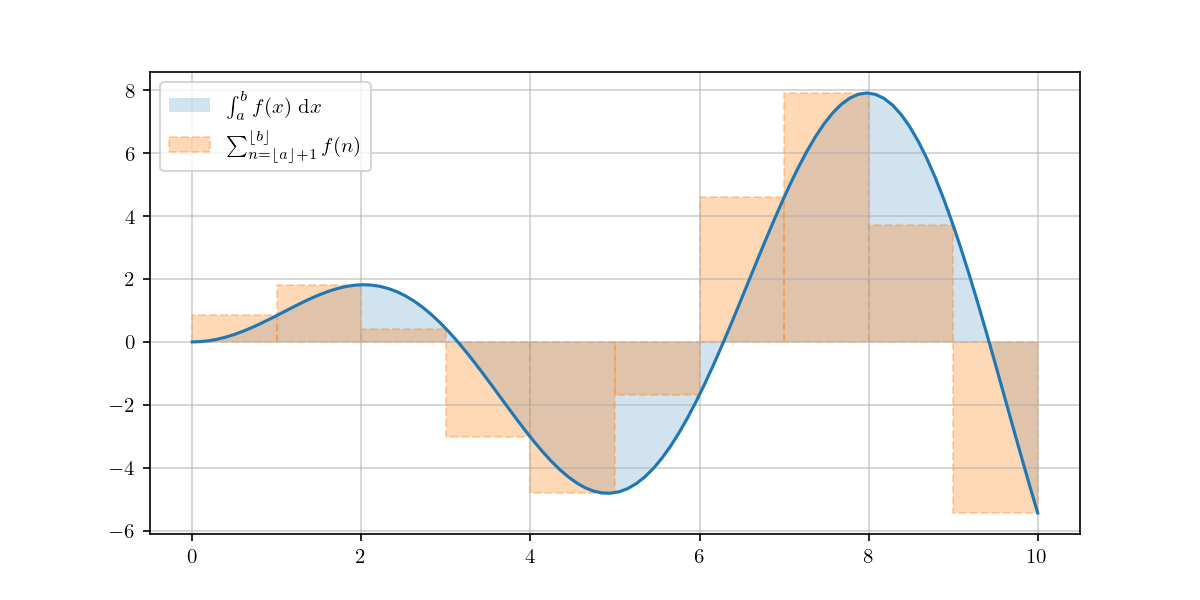
\includegraphics[width=0.7\textwidth]{figures/euler-summation-formula.png}
	\caption{Euler's Summation Formula.}
	\label{fig:6}
\end{figure}

\begin{theorem}[Euler's Summation Formula]
	If $f$ has a continuous derivative $f^\prime$ on $[a, b]$,
	then we have
	\begin{align}
		\sum_{n=\floor{a}+1}^{\floor{b}} f(n)
		= \int_a^b f(x) \dif x
		+ \int_a^b f^\prime(x) \{x\} \dif x
		+ f(a) \{a\} - f(b) \{b\}
		\label{eq:33}
	\end{align}

	In particular, if $a, b \in \Z$ we have
	\begin{align}
		\sum_{n=a+1}^{b} f(n)
		= \int_a^b f(x) \dif x
		+ \int_a^b f^\prime(x) \{x\} \dif x
		\label{eq:37}
	\end{align}
	By adding the term $f(a)$ on both sides and applying
	the fundamental theorem of calculus,
	one may obtain a more symmetric formula:
	\begin{align}
		\sum_{n=a}^b f(n)
		= \int_a^b f(x) \dif x
		+ \int_a^b f^\prime(x) \left( \{x\} - \frac{1}{2} \right) \dif x
		+ \frac{f(a) + f(b)}{2}
		\label{eq:38}
	\end{align}
\end{theorem}

\begin{note}
	\eqref{eq:37} is easier to use in practice while \eqref{eq:38}
	is more elegant in the sense of symmetry.
	To derive \eqref{eq:38}, we need to use the fundamental theorem of calculus,
	which will be introduced later.
\end{note}


\begin{proof}
	Consider a partition of $[\floor{a}+1, \floor{b}]$:
	\begin{align*}
		P = \{\floor{a}+1, \floor{a}+2, \ldots, \floor{b}\}
	\end{align*}
	Applying Theorem~\ref{thm:7}, we have
	\begin{align}
		\int_{\floor{a}+1}^{\floor{b}} f(x) \dif \floor{x}
		= \sum_{n=\floor{a}+2}^b f(n)
		\label{eq:29}
	\end{align}
	\begin{note}
		Note that $n$ starts at $\floor{a}+2$
		since the jump of the floor function $\floor{x}$
		at $x=\floor{a}+1$ is $0$.
	\end{note}

	Next, we examine the integrals $\int_a^{\floor{a}+1} f(x) \dif \floor{x}$
	and $\int_{\floor{b}}^b f(x) \dif \floor{x}$.
	It is clear that
	\begin{align}
		\int_{\floor{b}}^b f(x) \dif \floor{x} = 0
		\label{eq:30}
	\end{align}
	because it is zero be definition if $b \in \Z$
	and when $b \neq \Z$, $\floor{x} = \floor{b}$ is constant on $[\floor{b}, b]$.
	Now, we consider $\floor{x}$ on $[\floor{a}, \floor{a}+1]$.
	We have
	\begin{align*}
		\floor{x} = \begin{cases}
			            \floor{a},   & \floor{a} \leq x < \floor{a}+1 \\
			            \floor{a}+1, & x=\floor{a}+1
		            \end{cases}
	\end{align*}
	Therefore, $\floor{x}$ has a jump $1$ at $x=\floor{a}+1$.
	It then follows that
	\begin{align}
		\int_a^{\floor{a}+1} f(x) \dif \floor{x}
		= f(\floor{a}+1)
		\label{eq:31}
	\end{align}

	Combining \eqref{eq:29}, \eqref{eq:30} and \eqref{eq:31}, we obtain
	\begin{align}
		\int_a^b f(x) \dif \floor{x} = \sum_{n=\floor{a}+1}^b f(n)
		\label{eq:32}
	\end{align}
	This expresses the summation in \eqref{eq:33}
	as an integral.


	The rest of the proof leverages the theorems of
	integration by parts and reduction of Riemann integrals.
	Applying integration by parts, we have
	\begin{align}
		\int_a^b f(x) \dif x + \int_a^b x \dif f(x)
		= f(b)b - f(a)a
		\label{eq:34}
	\end{align}
	and
	\begin{align}
		\int_a^b f(x) \dif \floor{x} + \int_a^b \floor{x} \dif f(x)
		= f(b) \floor{b} - f(a) \floor{a}
		\label{eq:35}
	\end{align}
	Subtracting \eqref{eq:35} from \eqref{eq:34} yields
	\begin{align*}
		\int_a^b f(x) \dif x - \int_a^b f(x) \dif \floor{x}
		+ \int_a^b \{x\} \dif f(x)
		= f(b) \{b\} - f(a) \{a\}
	\end{align*}
	Since $f$ has a continuous derivative,
	by Theorem~\ref{thm:8},
	we can replace $\dif f(x)$
	with $f^\prime(x) \dif x$.
	Then rearranging the terms, we obtain
	\begin{align}
		\int_a^b f(x) \dif \floor{x}
		= \int_a^b f(x)\dif x
		+ \int_a^b f^\prime(x) \{x\} \dif x
		+ f(a) \{a\} - f(b) \{b\}
		\label{eq:36}
	\end{align}
	\eqref{eq:33} is proved by comparing \eqref{eq:32} and \eqref{eq:36}.
\end{proof}

\begin{example}
	Using the Euler's summation formula \eqref{eq:37},
	we can derive the following
	identities related to summing up terms of the form $\frac{1}{k^s}$:
	\begin{enumerate}
		\item If $s \neq 1$
		      \begin{align*}
			      \sum_{k=1}^n \frac{1}{k^s} = \frac{1}{n^{s-1}} + s \int_1^n \frac{\floor{x}}{x^{s+1}} \dif x
		      \end{align*}
		\item If $s=1$
		      \begin{align}
			      \sum_{k=1}^n \frac{1}{k}
			      = \ln n - \int_1^n \frac{\{x\}}{x^{2}} \dif x + 1
			      \label{eq:39}
		      \end{align}
	\end{enumerate}

	\eqref{eq:39} provides another way of
	proving
	the sequence $\left\{ \sum_{1}^n \frac{1}{k} - \ln n\right\}$ converges
	(to Euler's constant $\gamma$).
	And hence, we obtain an integral form of the Euler's constant:
	\begin{align*}
		\gamma = 1 - \int_1^\infty\ \frac{\{x\}}{x^2} \dif x
	\end{align*}
\end{example}


%------------------------------


\section{Darboux Integration -- Defining Integrals with Upper and Lower Integrals}

From now on, the theory of Riemann-Stieltjes integration
will be developed for increasing integrators.

One may have the feeling that
it is troublesome to prove the existence of Integrals
because not only are we required to find a partition
but also consider all possible choices $T$ of points in subintervals.

The definition of upper and lower sums
will get rid of $T$ in $S(P,T,f,\alpha)$.


\begin{definition}
	Let $P=\{x_0, x_1, \ldots, x_n\}$ be a partition of $[a, b]$.
	For $k=1, \ldots, n$, define
	\begin{align*}
		M_k(f) & := \sup_{x \in [x_{k-1}, x_{k}]} f(x) \\
		m_k(f) & := \inf_{x \in [x_{k-1}, x_k]} f(x)
	\end{align*}
	The sums
	\begin{align*}
		U(P, f, \alpha) & := \sum_{k=1}^n M_k(f) \Delta\alpha_k \\
		L(P, f, \alpha) & := \sum_{k=1}^n m_k(f) \Delta\alpha_k
	\end{align*}
	are called \textbf{upper and lower Darboux sums}\index{upper Darboux sum}\index{lower Darboux sum} respectively.
\end{definition}

Let $t_k \in [x_{k-1}, x_k]$, clearly, we have
\begin{align*}
	m_k(f) \leq f(t_k) \leq M_k
\end{align*}
If the integrator $\alpha$ is increasing, then
\begin{align*}
	m_k(f) \Delta \alpha_k \leq f(t_k) \Delta \alpha_k \leq M_k \Delta \alpha_k
\end{align*}
Summing over $k$ yields
\begin{align*}
	L(P, f, \alpha) \leq S(P, T, f, \alpha) \leq U(P, f, \alpha)
\end{align*}

\begin{theorem} \label{thm:9}
	Assume $\alpha$ is increasing on $[a, b]$. Then
	\begin{enumerate}
		\item if $P^\prime \supseteq P$,  we have
		      \begin{align*}
			      U(P^\prime, f, \alpha) \leq U(P, f, \alpha)
			      \quad \text{and} \quad
			      L(P^\prime, f, \alpha) \geq L(P, f, \alpha)
		      \end{align*}
		      In other words, as the partition gets finer the upper Darboux sum decreases
		      while the lower Darboux sum increases.
		\item For any two partitions $P_1$ and $P_2$, we have
		      \begin{align*}
			      L(P_1, f, \alpha) \leq U(P_2, f, \alpha)
		      \end{align*}
		      That is, any lower Darboux sum is no greater than any upper Darboux sum.
	\end{enumerate}
\end{theorem}

Think about how to prove $U(P^\prime, f, \alpha) \leq U(P, f, \alpha)$ in 1.
One way to do this is by designing notations to
explicitly write down
the expressions for $P^\prime$ and $U(P^\prime, f, \alpha)$.
My way is as follows.
Let $P = \{x_0, \ldots, x_n\}$.
Since $P \supseteq P$, we can express $P^\prime$ as
\begin{alignat*}{2}
	P^\prime & = & \{ & y_{0},                           \\
	         &   &    & y_{1}, \ldots y_{m_1},           \\
	         &   &    & \ldots,                          \\
	         &   &    & y_{m_{k-1}+1}, \ldots y_{m_k},   \\
	         &   &    & \ldots,                          \\
	         &   &    & y_{m_{n-1}+1}, \ldots y_{m_n} \}
\end{alignat*}
where $y_{m_k} = x_k$ ($m_0 = 0$) for $k=0, 1, \ldots, n$.
And we have
\begin{align*}
	U(P^\prime, f, \alpha)
	= \sum_{k=1}^n \sum_{j=m_{k-1} + 1}^{m_k}
	\sup_{x \in [y_{j-1}, y_{j}]}
	f(x) [\alpha(y_{j}) - \alpha(y_{j-1})]
\end{align*}
And the rest of the proof can be done easily.

However, we can be a little smarter about this proof.
Note that the major difficulty is that
the form of the refinement $P^\prime$
is undetermined.
It may contain many extra points scattered in different locations.
But we can start by consider the simplest case
where $P^\prime$ has only one point more than $P$.
And then we can extend the conclusion to any
larger refinements by applying the mathematical induction.

\begin{proof}
	\noindent\textbf{Proof of 1:}
	We only prove $U(P^\prime, f, \alpha) \leq U(P, f, \alpha)$.
	First, consider the case where $P^\prime$
	has only one point $y$ more than $P = \{x_0, \ldots, x_n\}$.
	Suppose $y \in (x_{j-1}, x_j)$.
	On the subinterval $[x_{j-1}, x_j]$, we have
	\begin{multline*}
		\sup_{x \in [x_{j-1}, y]} f(x) [\alpha(y) - \alpha(x_{j-1})]
		+ \sup_{x \in [y, x_j]} f(x) [\alpha(x_{j}) - \alpha(y)] \\
		\leq \sup_{x \in [x_{j-1}, x_j]} f(x) [\alpha(x_{j}) - \alpha(x_{j-1})]
		= M_j
	\end{multline*}
	Then it is clear that $U(P^\prime, f, \alpha) \leq U(P, f, \alpha)$.

	In general, suppose $\abs{P^\prime} = \abs{P} + n$,
	one may then prove this easily by
	applying the mathematical induction.


	\noindent\textbf{Proof of 2:}
	Let $P = P_1 \cup P_2$.
	Then $P$ is a refinement of both $P_1$ and $P_2$.
	Applying the first part of this theorem and the inequality that
	\begin{align*}
		L(P, f, \alpha) \leq U(P, f, \alpha)
	\end{align*}
	we obtain
	\begin{align*}
		L(P_1, f, \alpha) \leq L(P, f, \alpha) \leq U(P, f, \alpha)
		\leq U(P_2, f, \alpha)
	\end{align*}
\end{proof}

Let $P_0 = \{a, b\}$ be the trivial partition on $[a, b]$.
Then $U(P, f, \alpha) \geq L(P_0, f, \alpha)$
and $L(P, f, \alpha) \leq U(P_0, f, \alpha)$ for every partition $P$,
which means that the set of all upper Darboux sums is bounded below,
and the set of all lower Darboux sums is bounded above.
Then we may take the infimum and supremum, respectively, of the two sets
to introduce the definitions of the upper and lower integrals.


\begin{definition}
	Assume $\alpha$ is increasing on $[a, b]$.
	The \textbf{upper Darboux integral}\index{upper Darboux integral}
	is defined by
	\begin{align*}
		\overline{\int_a^b} f \dif \alpha
		:= \inf_{P \in \CALP[a, b]} U(P, f, \alpha)
	\end{align*}
	and the  \textbf{lower Darboux integral}\index{lower Darboux integral}
	is defined by
	\begin{align*}
		\underline{\int_a^b} f \dif \alpha
		:= \sup_{P \in \CALP[a, b]} L(P, f, \alpha)
	\end{align*}
\end{definition}

\begin{note}
	Upper and lower integrals always exist
	assuming $f$ is bounded and $\alpha$ is increasing, of course.
\end{note}

Intuitively, the lower integral should be no greater than the upper integral.

\begin{theorem}
	Assume $\alpha$ is increasing on $[a, b]$, we have
	\begin{align}
		\underline{\int_a^b} f \dif \alpha
		\leq \overline{\int_a^b} f \dif \alpha
		\label{eq:40}
	\end{align}
\end{theorem}

\begin{proof}
	Let $\varepsilon > 0$ be arbitrary.
	By the property of infimums, there exists a partition $P_1$ of $[a, b]$
	such that
	\begin{align*}
		\underline{\int_a^b} f \dif \alpha
		< L(P_1, f, \alpha) + \varepsilon/2
	\end{align*}
	Similarly, by the property of supremums,
	there exists a partition $P_2$ of $[a, b]$
	such that
	\begin{align*}
		\overline{\int_a^b} f \dif \alpha
		> U(P_2, f, \alpha) - \varepsilon/2
	\end{align*}
	It then follows that
	\begin{align*}
		\underline{\int_a^b} f \dif \alpha
		 & < L(P_1, f, \alpha) + \varepsilon/2                                 \\
		 & \leq U(P_2, f, \alpha) + \varepsilon/2                              \\
		 & < \overline{\int_a^b} f \dif \alpha + \varepsilon/2 + \varepsilon/2 \\
		 & = \overline{\int_a^b} f \dif \alpha + \varepsilon
	\end{align*}
	In summary, we have
	\begin{align*}
		\underline{\int_a^b} f \dif \alpha
		< \overline{\int_a^b} f \dif \alpha + \varepsilon
		\quad \forall \varepsilon > 0
	\end{align*}
	This implies that $\underline{\int_a^b} f \dif \alpha \leq \overline{\int_a^b} f \dif \alpha$.
\end{proof}

There are examples where the inequality in \eqref{eq:40} is strict.

\begin{example}
	Consider the Dirichlet function $\ind_{\Q}(x)$ restricted on $[a, b]$.
	Let $P$ an arbitrary partition of $[a, b]$.
	On any subinterval $[x_{k-1}, x_k]$, we have
	\begin{align*}
		\sup_{[x_{k-1}, x_k]} \ind_{\Q}(x) = 1
		\quad \text{and} \quad
		\inf_{[x_{k-1}, x_k]} \ind_{\Q}(x) = 0
	\end{align*}
	It then follows that
	\begin{align*}
		U(P, \ind_\Q, x) = b - a
		\quad \text{and} \quad
		L(P, \ind_\Q, x) = 0
	\end{align*}
	Since the above equations hold for all $P \in \CALP[a, b]$,
	the upper and lower integrals are
	\begin{align*}
		\overline{\int_a^b} \ind_{\Q}(x) \dif x = b - a
		\quad \text{and} \quad
		\underline{\int_a^b} \ind_{\Q}(x) \dif x = 0
	\end{align*}
\end{example}



\section{Additive and Linearity Properties of Upper and Lower Integrals}

\begin{proposition}
	Let $c\in (a, b)$.
	We have the following identities for upper and lower integrals:
	\begin{align*}
		\overline{\int_a^b} f \dif \alpha
		= \overline{\int_a^c} f \dif \alpha + \overline{\int_c^b} f \dif \alpha
	\end{align*}
	and
	\begin{align*}
		\underline{\int_a^b} f \dif \alpha
		= \underline{\int_a^c} f \dif \alpha + \underline{\int_c^b} f \dif \alpha
	\end{align*}
\end{proposition}

\begin{proof}
	We only prove the identity for upper integrals.
	We will prove this identity by showing both
	LHS $\geq$ RHS and LHS $\leq$ RHS.

	\noindent\textbf{Proof of LHS $\geq$ RHS:}
	Let $P_1$ and $P_2$ be partitions of $[a, c]$ and $[c, b]$, respectively.
	Let $P = P_1 \cup P_2$.
	We have
	\begin{align*}
		U(P, f, \alpha) = U(P_1, f, \alpha) + U(P_2, f, \alpha)
		\geq \overline{\int_a^c} f \dif \alpha + \overline{\int_c^b} f \dif \alpha
	\end{align*}
	Taking the infimum over $P$ yields
	\begin{align*}
		\overline{\int_a^b} f \dif \alpha
		= \inf_{P \in \CALP[a, b]} U(P, f, \alpha)
		\geq \overline{\int_a^c} f \dif \alpha + \overline{\int_c^b} f \dif \alpha
	\end{align*}


	\noindent\textbf{Proof of LHS $\leq$ RHS:}
	Let $\varepsilon > 0$ be arbitrary.
	There exist a partition $P_1$ of $[a, c]$ and a partition $P_2$ of $[c, b]$
	such that
	\begin{align*}
		U(P_1, f, \alpha) - \varepsilon / 2 & < \overline{\int_a^c} f \dif \alpha \\
		U(P_2, f, \alpha) - \varepsilon / 2 & < \overline{\int_c^b} f \dif \alpha
	\end{align*}
	Let $P = P_1 \cup P_2$.
	Adding the above two inequalities yields
	\begin{align*}
		U(P, f, \alpha) - \varepsilon
		= U(P_1, f, \alpha) - \varepsilon/2
		+ U(P_2, f, \alpha) - \varepsilon/2
		< \overline{\int_a^c} f \dif \alpha
		+ \overline{\int_c^b} f \dif \alpha
	\end{align*}
	Taking the infimum over $P$ on both sides yields
	\begin{align*}
		\overline{\int_a^b} f \dif \alpha - \varepsilon
		= \inf_{P \in \CALP[a, b]} (U(P, f, \alpha) - \varepsilon)
		\leq \overline{\int_a^c} f \dif \alpha
		+ \overline{\int_c^b} f \dif \alpha
	\end{align*}
	Since
	\begin{align*}
		\overline{\int_a^b} f \dif \alpha - \varepsilon
		\leq \overline{\int_a^c} f \dif \alpha
		+ \overline{\int_c^b} f \dif \alpha
	\end{align*}
	holds for every $\varepsilon > 0$,
	\begin{align*}
		\overline{\int_a^b} f \dif \alpha
		\leq \overline{\int_a^c} f \dif \alpha
		+ \overline{\int_c^b} f \dif \alpha
	\end{align*}
\end{proof}

\begin{proposition}
	We have the following inequalities
	about upper and lower integrals of sums of two functions:
	\begin{align}
		\overline{\int_a^b} f+g \dif \alpha
		\leq \overline{\int_a^b} f \dif \alpha
		+ \overline{\int_a^b} g \dif \alpha
		\label{eq:41}
	\end{align}
	and
	\begin{align*}
		\underline{\int_a^b} f+g \dif \alpha
		\geq \underline{\int_a^b} f \dif \alpha
		+ \underline{\int_a^b} g \dif \alpha
	\end{align*}
\end{proposition}

\begin{proof}
	We only prove \eqref{eq:41}.
	Let $P$ be any partition of $[a, b]$.
	On each interval $[x_{k-1}, x_k]$, we have
	\begin{align*}
		f(x) + g(x)
		\leq \sup_{x \in [x_{k-1}, x_k]} f(x)
		+ \sup_{x \in [x_{k-1}, x_k]} g(x)
		\quad \forall x \in [x_{k-1}, x_k]
	\end{align*}
	Taking the supremum on both sides over $x$ yields
	\begin{align*}
		\sup_{x \in [x_{k-1}, x_k]} f(x) + g(x)
		\leq \sup_{x \in [x_{k-1}, x_k]} f(x)
		+ \sup_{x \in [x_{k-1}, x_k]} g(x)
	\end{align*}
	Then summing over $k$:
	\begin{align*}
		U(P, f+g, \alpha)
		 & = \sum_{k} \sup_{x \in [x_{k-1}, x_k]} f(x) + g(x) \\
		 & \leq \sum_{k} \sup_{x \in [x_{k-1}, x_k]} f(x)
		+ \sum_{k} \sup_{x \in [x_{k-1}, x_k]} g(x)           \\
		 & = U(P, f, \alpha) + U(P, g, \alpha)
	\end{align*}
	Finally, the inequality is proved by
	taking the infimum on both sides over $P$.
\end{proof}

\begin{example}
	The inequality \eqref{eq:41} may be strict.
	Consider $f(x) = \ind_{\Q} (x)$ and $g(x) = -\ind_{\Q}(x)$
	restricted on $[a, b]$.
	We have
	\begin{align*}
		\overline{\int_a^b} f+g \dif \alpha
		= \overline{\int_a^b} 0 \dif \alpha
		= 0
	\end{align*}
	and
	\begin{align*}
		\overline{\int_a^b} f \dif \alpha = b-a
		\quad \text{and} \quad
		\overline{\int_a^b} g \dif \alpha = 0
	\end{align*}
\end{example}



\section{Riemann's Condition}

When we are discussing about whether
the limit $\lim$ exists or not,
we check that if
the limit inferior $\liminf$
and the limit superior $\limsup$
are equal.

Similarly, it is reasonable to guess that
the existence of the integral $\int$ depends on
the equality of the lower and upper integrals
(whether $\underline{\int} = \overline{\int}$).


\begin{definition}
	We say that a function $f$
	satisfies the \textbf{Riemann's condition}\index{Riemann's condition}
	with respect to $\alpha$ on $[a, b]$
	if for any $\varepsilon > 0$,
	there exists a partition $P_\varepsilon$ such that
	\begin{align}
		P \supseteq P_\varepsilon
		\implies
		0 \leq U(P, f, \alpha) - L(P, f, \alpha) < \varepsilon
		\label{eq:42}
	\end{align}
	or equivalently, just saying that
	\begin{align}
		0 \leq U(P_\varepsilon, f, \alpha) - L(P_\varepsilon, f, \alpha) < \varepsilon
		\label{eq:43}
	\end{align}
\end{definition}

\begin{note}
	\eqref{eq:42} is the definition given in \cite{apostolMathematicalAnalysisModern1974}.
	But clearly \eqref{eq:42} $\iff$ \eqref{eq:43}.
	(\eqref{eq:42} $\implies$ \eqref{eq:43} is obvious.)
	If \eqref{eq:43} holds,
	then by Theorem~\ref{thm:9}
	we know that the upper sum will decrease while the lower sum will increase
	as the partition gets finer,
	and the lower sum is always no greater than the upper sum.
	Therefore, \eqref{eq:42} holds.
\end{note}

\begin{proposition} \label{prop:7}
	Let $f$ be a bounded function on $[a, b]$. We have
	\begin{align*}
		\sup_{x, y \in [a, b]} [f(x) - f(y)]
		= \sup_{x \in [a, b]} f(x) - \inf_{x \in [a, b]} f(x)
	\end{align*}
\end{proposition}

\begin{proof}
	Let $M = \sup_{x \in [a, b]} f(x)$ and $m = \inf_{x \in [a, b]} f(x)$.
	Clearly
	\begin{align*}
		f(x) - f(y) \leq M - m \quad \forall x, y \in [a, b]
	\end{align*}
	That is, $M-m$ is an upper bound of the
	set $\{f(x) - f(y) \mid x, y \in [a, b]\}$.
	We now show that $M - m$ is the least upper bound.
	Let $\varepsilon > 0$ be arbitrary.
	There exists $x_0 \in [a, b]$ such that $f(x_0) > M - \varepsilon/2$,
	and there exists $y_0 \in [a, b]$ such that $f(y_0) < m + \varepsilon/2$.
	It then follows that
	\begin{align*}
		f(x_0) - f(y_0) > M - m - \varepsilon
	\end{align*}
	This completes the proof.
\end{proof}

The following theorem ease the procedure of proving
the existence of an integral.

\begin{theorem}
	Assume $\alpha$ is increasing on $[a, b]$.
	Then the following statements are equivalent:
	\begin{enumerate}
		\item $f \in \mathfrak{R}(\alpha)$ on $[a, b]$.
		\item $f$ satisfies the Riemann's condition with respect to $\alpha$ on $[a, b]$.
		\item $\underline{\int_a^b} f \dif \alpha = \overline{\int_a^b} f \dif \alpha$.
	\end{enumerate}
\end{theorem}

\begin{proof}
	\noindent\textbf{Proof of 1 $\implies$ 2:}
	Let $\varepsilon > 0$ be arbitrary.
	Because $f \in \mathfrak{R}(\alpha)$ on $[a, b]$,
	there exists a partition $P_\varepsilon$ such that
	for all $P \supseteq P_\varepsilon$
	and any list of representatives $T$ of $P$, we have
	\begin{align}
		\abs{ S(P, T, f, \alpha) - \int_a^b f \dif \alpha } < \varepsilon / 4
		\label{eq:44}
	\end{align}

	We now construct two particular lists of representatives
	$T_1$ and $T_2$ of $P$ as follows.
	Write $P = \{x_0, \ldots, x_n\}$.
	On each subinterval $[x_{k-1}, x_k]$,
	we can find a $t_k$ such that
	\begin{align*}
		f(t_k) \Delta \alpha_k < m_k + \frac{\varepsilon}{4n}
	\end{align*}
	and we can find a $t_k^\prime$ such that
	\begin{align*}
		f(t_k^\prime) \Delta \alpha_k > M_k - \frac{\varepsilon}{4n}
	\end{align*}
	Let $T_1$ be the list of all such $t_k$'s
	and $T_2$ be the list of all $t_k^\prime$'s.
	It then follows that
	\begin{align*}
		S(P, T_1, f, \alpha) & < L(P, f, \alpha) + \varepsilon / 4 \\
		S(P, T_2, f, \alpha) & > U(P, f, \alpha) - \varepsilon / 4
	\end{align*}
	Taking the difference yields
	\begin{align}
		U(P, f, \alpha) - L(P, f, \alpha)
		< S(P, T_1, f, \alpha) - S(P, T_2, f, \alpha) + \varepsilon/2
		\label{eq:45}
	\end{align}

	But \eqref{eq:44} implies that
	\begin{align*}
		\abs{S(P, T_1, f, \alpha) - S(P, T_2, f, \alpha)} < \varepsilon/2
	\end{align*}
	Combined with \eqref{eq:45}, we obtain
	\begin{align*}
		U(P, f, \alpha) - L(P, f, \alpha) < \varepsilon
	\end{align*}
	which holds for any refinement $P$ of $P_\varepsilon$.
	Therefore, $f$ satisfies the Riemann's condition
	with respect to $\alpha$ on $[a, b]$.

	\noindent\textbf{Proof of 2 $\implies$ 3:}
	Let $\varepsilon > 0$ be arbitrary.
	Because $f$ satisfies the Riemann's condition.
	There exists a partition $P_\varepsilon$ such that
	\begin{align*}
		U(P_\varepsilon, f, \alpha) - L(P_\varepsilon, f, \alpha) < \varepsilon
	\end{align*}
	But
	\begin{align*}
		0 \leq \overline{\int_a^b} f \dif \alpha
		- \underline{\int_a^b} f \dif \alpha
		\leq U(P_\varepsilon, f, \alpha) - L(P_\varepsilon, f, \alpha)
	\end{align*}
	Therefore,
	\begin{align*}
		0 \leq \overline{\int_a^b} f \dif \alpha
		- \underline{\int_a^b} f \dif \alpha < \varepsilon
	\end{align*}
	Since the above inequality holds for every $\varepsilon$,
	we have $ \underline{\int_a^b} f \dif \alpha = \overline{\int_a^b} f \dif \alpha$.


	\noindent\textbf{Proof of 3 $\implies$ 1:}
	Let $\varepsilon > 0$ be arbitrary.
	There exists a partition $P_\varepsilon^\prime$ such that
	\begin{align*}
		\overline{\int_a^b} f \dif \alpha + \varepsilon
		> U(P_\varepsilon^\prime, f, \alpha)
	\end{align*}
	and a partition $P_\varepsilon^{\prime\prime}$ such that
	\begin{align*}
		\underline{\int_a^b} f \dif \alpha - \varepsilon
		< L(P_\varepsilon^{\prime\prime}, f, \alpha)
	\end{align*}
	Let $P_\varepsilon = P_\varepsilon^\prime \cup P_\varepsilon^{\prime\prime}$.
	For any refinement $P \supseteq P_\varepsilon$,
	and any list of representatives $T$ of $P$,
	we have
	\begin{align*}
		\underline{\int_a^b} f \dif \alpha - \varepsilon
		< L(P, f, \alpha)
		\leq S(P, T, f, \alpha)
		\leq U(P, f, \alpha)
		< \overline{\int_a^b} f \dif \alpha + \varepsilon
	\end{align*}
	Because the lower and upper integrals are equal,
	we can write $A = \underline{\int_a^b} f \dif \alpha - \varepsilon = \overline{\int_a^b} f \dif \alpha - \varepsilon$.
	It then follows that
	\begin{align*}
		\abs{ S(P, T, f, \alpha) - A } < \varepsilon
	\end{align*}
	This implies that $f \in \mathfrak{R}(\alpha)$ on $[a, b]$,
	and the value of the integral
	equals to that of both lower and upper integrals.
\end{proof}


\section{Comparison Theorems}

\begin{theorem}
	Assume $\alpha$ is increasing and $f \geq 0$ on $[a, b]$.
	If $f \in \mathfrak{R}(\alpha)$, then
	\begin{align*}
		\int_a^b f \dif \alpha \geq 0
	\end{align*}
\end{theorem}

\begin{proof}
	Let $P$ be any partition of $[a, b]$.
	On any subinterval $[x_{k-1}, x_k]$,
	we have $f(x) \geq 0$ and hence
	\begin{align*}
		\sup_{[x_{k-1}, x_k]} f(x) \Delta \alpha_k \geq 0
	\end{align*}
	Summing up over $k$, we obtain
	\begin{align*}
		U(P, f, \alpha) \geq 0
	\end{align*}
	Finally, taking the infimum over $P$ yields
	\begin{align*}
		\overline{\int_a^b} f \dif \alpha \geq 0
	\end{align*}
	Because $f \in \mathfrak{R}(\alpha)$,
	its integral equals to the upper integral,
	hence greater than or equal to zero.
\end{proof}

\begin{corollary} \label{cor:2}
	Assume $\alpha$ is increasing and $f \leq g$ on $[a, b]$.
	If $f, g \in \mathfrak{R}(\alpha)$, then
	\begin{align*}
		\int_a^b f \dif \alpha \leq \int_a^b g \dif \alpha
	\end{align*}
\end{corollary}

\begin{theorem} \label{thm:28}
	Assume $\alpha$ is increasing on $[a, b]$.
	If $f \in \mathfrak{R}(\alpha)$ on $[a, b]$,
	then $\abs{f} \in \mathfrak{R}(\alpha)$ on $[a, b]$, and
	\begin{align}
		\abs{\int_a^b f \dif \alpha} \leq \int_a^b \abs{f} \dif \alpha
		\label{eq:47}
	\end{align}
\end{theorem}

\begin{proof}
	Let $\varepsilon > 0$ be arbitrary.
	Because $f \in \mathfrak{R}(\alpha)$ on $[a, b]$
	equivalently, satisfying the Riemann's condition,
	there exists a partition $P_\varepsilon = \{x_0, \ldots, x_n\}$
	such that $U(P, f, \alpha) - L(P, f, \alpha) < \varepsilon$.
	On each subinterval $I_k = [x_{k-1}, x_k]$, we have
	\begin{align*}
		\omega_{\abs{f}}(I_k)
		= \sup_{x, y \in I_k} ( \abs{f(x)} - \abs{f(y)} )
		\leq \sup_{x, y \in I_k} \abs{ f(x) - f(y) }
		= \omega_f(I_k)
	\end{align*}
	Multiplying by $\Delta \alpha_k$ on both sides and then summing over $k$,
	we obtain
	\begin{align*}
		U(P_\varepsilon, \abs{f}, \alpha) - L(P_\varepsilon, \abs{f}, \alpha)
		 & = \sum_{k=1}^n \omega_{\abs{f}}(I_k) \Delta \alpha_k        \\
		 & \leq \sum_{k=1}^n \omega_{f}(I_k) \Delta \alpha_k           \\
		 & = U(P_\varepsilon, f, \alpha) - L(P_\varepsilon, f, \alpha) \\
		 & < \varepsilon
	\end{align*}
	This implies that $\abs{f}$ also satisfies the Riemann's condition
	and hence integrable.

	Then, since $-\abs{f} \leq f \leq \abs{f}$, \eqref{eq:47}
	is proved by applying Corollary~\ref{cor:2}.
\end{proof}


\begin{example}
	If $\abs{f}$ is integrable then $f$ does not need to be integrable.
	Consider a function $f$  on $[a, b]$ defined by
	\begin{align*}
		f(x) = \ind_{\Q}(x) - \ind_{\R \setminus \Q}(x)
		= \begin{cases}
			  1  & x \in \Q    \\
			  -1 & x \notin \Q
		  \end{cases}
	\end{align*}
	We have $\abs{f(x)} = 1$, which is a constant and hence integrable.
	But $f$ is not.
\end{example}

\begin{theorem} \label{thm:10}
	Assume $\alpha$ is increasing on $[a, b]$.
	If $f \in \mathfrak{R}(\alpha)$ on $[a, b]$
	then $f^2 \in \mathfrak{R}(\alpha)$ on $[a, b]$.
\end{theorem}

\begin{proof}
	Suppose $f$ is bounded by $M > 0$ on $[a, b]$.
	Let $\varepsilon > 0$ be arbitrary.
	Because $f \in \mathfrak{R}(\alpha)$ on $[a, b]$,
	there exists a partition $P_\varepsilon$ of $[a, b]$
	such that
	\begin{align*}
		U(P_\varepsilon, f, \alpha) - L(P_\varepsilon, f, \alpha)
		< \frac{\varepsilon}{2M}
	\end{align*}
	We are going to show that $f^2$ also satisfies the Riemann's condition.

	On each subinterval $I_k$, we have
	\begin{align*}
		\abs{f^2(x) - f^2(y)}
		 & = \abs{f(x) + f(y)} \abs{f(x) - f(y)}         \\
		 & \leq 2M \sup_{x, y \in I_k} \abs{f(x) - f(y)} \\
		 & = 2M \omega_f(I_k)
	\end{align*}
	It then follows that
	\begin{align*}
		\omega_{f^2}(I_k)
		= \sup_{x, y \in I_k} \abs{f^2(x) - f^2(y)}
		\leq 2M \omega_f(I_k)
	\end{align*}
	Multiplying by $\Delta \alpha_k$ and then summing over $k$ yields
	\begin{align*}
		U(P_\varepsilon, f^2, \alpha) - L(P_\varepsilon, f^2, \alpha)
		 & = \sum_{k} \omega_{f^2}(I_k) \Delta \alpha_k                     \\
		 & \leq 2M \sum_{k} \omega_f(I_k) \Delta \alpha_k                   \\
		 & = 2M [U(P_\varepsilon, f, \alpha) - L(P_\varepsilon, f, \alpha)] \\
		 & < 2M \frac{\varepsilon}{2M}                                      \\
		 & = \varepsilon
	\end{align*}
\end{proof}

An immediate consequence of the previous theorem is that
the product of integrable functions is also integrable.

\begin{theorem} \label{thm:14}
	Assume $\alpha$ is increasing on $[a, b]$.
	If $f, g \in \mathfrak{R}(\alpha)$ on $[a, b]$
	then the product is also integrable: $fg \in \mathfrak{R}(\alpha)$ on $[a, b]$.
\end{theorem}

\begin{proof}
	The product $fg$ can be written as
	\begin{align*}
		fg = \frac{1}{4}[ (f+g)^2 - (f-g)^2 ]
	\end{align*}
	Because the sum and difference $f \pm g$ are integrable,
	so do their squares $(f \pm g)^2$ by the previous theorem.
	Therefore, $fg \in \mathfrak{R}(\alpha)$ on $[a, b]$.
\end{proof}


\section{Integrators of Bounded Variation}

Recall in the previous section we always assume that
the integrator $\alpha$ is increasing.
Now, we want to extend the theorems about existence of integrals
to the case when the integrator is of bounded variation.

For example, we want to generalize Theorem~\ref{thm:10} to
that assuming $\alpha$ is of bounded variation on $[a, b]$,
if $f \in \mathfrak{R}(\alpha)$ on $[a, b]$,
then $f^2 \in \mathfrak{R}(\alpha)$ on $[a, b]$.

The key of achieving this is that a function $\alpha$ of bounded variation
can be written as a difference of
two increasing functions $\alpha_1$ and $\alpha_2$,
(Theorem~\ref{thm:4}).
\begin{align*}
	\alpha = \alpha_1 - \alpha_2
\end{align*}
Then, to exploit the condition that $f \in \mathfrak{R}(\alpha)$,
we would want that $f \in \mathfrak{R}(\alpha_1)$ and $f \in \mathfrak{R}(\alpha_2)$.
But this is not true in general due to the nonuniqueness
of the decomposition of $\alpha$ into two increasing functions.
For example, consider $\alpha(x) = 0$ on $[a, b]$.
We can write $\alpha$ as a difference of two identity
functions $\alpha_1(x) = \alpha(x) = x$.
Then the Dirichlet function $\ind_{\Q}$ is not integrable
w.r.t. $\alpha_1$ nor $\alpha_2$.
But it is integrable w.r.t. $\alpha$ for the integrator is constant.

However, if we decompose $\alpha$ (in the canonical way) as
\begin{align*}
	\alpha(x) = V_a^x(\alpha) - [ V_a^x(\alpha) - \alpha(x) ]
\end{align*}
then we will see in Theorem~\ref{thm:11} that $f$
is also integrable w.r.t. $V_a^x(\alpha)$ and $V_a^x(\alpha) - \alpha(x)$.



\begin{lemma} \label{lem:1}
	Assume $\alpha$ is of bounded variation on $[a, b]$.
	If $f \in \mathfrak{R}(\alpha)$ on $[a, b]$,
	then for any given $\varepsilon > 0$
	there exists a partition $P_\varepsilon$ of $[a, b]$ such that
	for all refinement $P \supseteq P_\varepsilon$, $P = \{x_0, \ldots, x_n\}$,
	we have
	\begin{align}
		\sum_{k=1}^n \omega_f(I_k) \abs{\Delta \alpha_k} < \varepsilon
		\label{eq:48}
	\end{align}
\end{lemma}

\begin{note}
	If $\alpha$ is increasing,
	then what this lemma states is exactly
	that $f$ satisfies the Riemann's condition.
\end{note}

The idea of the proof is as follows.
The appearance of the oscillation $\omega_f(I_k)$ in \eqref{eq:48}
suggests us to consider the difference $f(t_k) - f(t^\prime_k)$.
We have for all $t_k, t^\prime_k \in [x_{k-1}, x_k]$ that
\begin{align*}
	\abs{\sum_{k=1}^n [ f(t_k) - f(t^\prime_k) ] \Delta \alpha_k} < c \varepsilon
\end{align*}
The difficulty is that $\Delta \alpha_k$ is not nonnegative anymore as
in the previous section.
To solve this, we simply
consider the set $A$ of indices of which $\Delta \alpha_k \geq 0$
and the set $B$ of indices of which $\Delta \alpha_k < 0$ separately.
Then we have
\begin{align*}
	\sum_{k=1}^n [ f(t_k) - f(t^\prime_k) ] \Delta \alpha_k
	= \sum_{k \in A} [ f(t_k) - f(t^\prime_k) ] \abs{\Delta \alpha_k}
	+ \sum_{k \in B} [ f(t_k^\prime) - f(t_k) ] \abs{\Delta \alpha_k}
\end{align*}
The rest of the proof is done by choosing the $t_k$ and $t^\prime_k$
and then comparing $\abs{f(t_k) - f(t^\prime_k)}$ with $\omega_f(I_k)$.

\begin{proof}
	If $V_a^b(\alpha) = 0$, then $\alpha$ is constant
	and hence the conclusion is trivial.
	In the following context, we assume $V_a^b(\alpha) > 0$.

	Let $\varepsilon > 0$ be arbitrary.
	Because $f \in \mathfrak{R}(\alpha)$ on $[a, b]$,
	there exists a partition $P_\varepsilon$ of $[a, b]$
	such that
	for any refinement $P=\{x_0, \ldots, x_n\}$
	and any list of representatives $T$ of $P$, we have
	\begin{align*}
		\abs{S(P, T, f, \alpha) - \int_a^b f \dif \alpha} < \varepsilon / 4
	\end{align*}
	It then follows that
	\begin{align*}
		\abs{\sum_{k=1}^n [ f(t_k) - f(t^\prime_k) ] \Delta \alpha_k} < \varepsilon / 2
		\quad \forall t_k, t^\prime_k \in [x_{k-1}, x_k]
	\end{align*}

	Let subsets $A$ and $B$ of indices $\{1, \ldots, n\}$ be defined by
	\begin{align*}
		A & = \set{\Delta \alpha_k \geq 0}{k \in \{1, \ldots, n\}} \\
		B & = \set{\Delta \alpha_k < 0}{k \in \{1, \ldots, n\}}
	\end{align*}
	Clearly, $A$ and $B$ forms a partition of $\{1, \ldots, n\}$,
	i.e., $A \cup B = \{1, \ldots, n\}$ and $A \cap B = \emptyset$.
	It then follows that
	\begin{align*}
		\sum_{k=1}^n [ f(t_k) - f(t^\prime_k) ] \Delta \alpha_k
		= \sum_{k \in A} [ f(t_k) - f(t^\prime_k) ] \abs{\Delta \alpha_k}
		+ \sum_{k \in B} [ f(t_k^\prime) - f(t_k) ] \abs{\Delta \alpha_k}
	\end{align*}
	Therefore,
	\begin{align}
		\abs{
			\sum_{k \in A} [ f(t_k) - f(t^\prime_k) ] \abs{\Delta \alpha_k}
			+ \sum_{k \in B} [ f(t_k^\prime) - f(t_k) ] \abs{\Delta \alpha_k}
		} < \varepsilon / 2
		\quad \forall t_k, t^\prime_k \in [x_{k-1}, x_k]
		\label{eq:49}
	\end{align}


	Now, we will strategically select $t_k$ and $t^\prime_k$
	to accomplish our goal.
	\begin{enumerate}
		\item For $k \in A$, we may select $t_k$ and $t^\prime_k$
		      such that $f(t_k) - f(t^\prime_k) > \max \left\{ 0, \omega_f(I_k) - \frac{\varepsilon}{2 V_a^b(\alpha)} \right\}$, and
		\item For $k \in B$, we may select $t_k$ and $t^\prime_k$
		      such that $f(t^\prime_k) - f(t_k) > \max \left\{ 0, \omega_f(I_k) - \frac{\varepsilon}{2 V_a^b(\alpha)} \right\}$.
	\end{enumerate}
	Plugging the particular choices of $t_k$'s and $t^\prime_k$'s
	into \eqref{eq:49}, we obtain
	\begin{align*}
		\varepsilon / 2
		 & > 	\abs{
			\sum_{k \in A} [ f(t_k) - f(t^\prime_k) ] \abs{\Delta \alpha_k}
			+ \sum_{k \in B} [ f(t_k^\prime) - f(t_k) ] \abs{\Delta \alpha_k}
		}                                                                           \\
		 & = 	\sum_{k \in A} [ f(t_k) - f(t^\prime_k) ] \abs{\Delta \alpha_k}
		+ \sum_{k \in B} [ f(t_k^\prime) - f(t_k) ] \abs{\Delta \alpha_k}           \\
		 & > \sum_{k=1}^n \left(
		\omega_f(I_k) - \frac{\varepsilon}{2 V_a^b(\alpha)}
		\right) \abs{\Delta \alpha_k}                                               \\
		 & =  \sum_{k=1}^n \omega_f(I_k) \abs{\Delta \alpha_k}
		- \frac{\varepsilon}{2 V_a^b(\alpha)} \sum_{k=1}^n \abs{\Delta \alpha_k}    \\
		 & \geq  \sum_{k=1}^n \omega_f(I_k) \abs{\Delta \alpha_k} - \varepsilon / 2
	\end{align*}
	where the last inequality follows from the property of
	total variations $\sum_{k=1}^n \abs{\Delta \alpha_k} \leq V_a^b(\alpha)$.
	Moving the term $-\varepsilon / 2$ to the left in the above inequality yields
	\begin{align*}
		\sum_{k=1}^n \omega_f(I_k) \abs{\Delta \alpha_k} < \varepsilon
	\end{align*}
\end{proof}


\begin{theorem} \label{thm:11}
	Assume $\alpha$ is of bounded variation on $[a, b]$.
	If $f \in \mathfrak{R}(\alpha)$ on $[a, b]$
	then $f \in \mathfrak{R}(V_a^x(\alpha))$ on $[a, b]$.

	And of course, applying the linearity,
	we also have $f \in \mathfrak{R}(V_a^x(\alpha) - \alpha)$ on $[a, b]$.
\end{theorem}

\begin{proof}
	Suppose $f$ is bounded by $M > 0$.

	Let $\varepsilon > 0$ be arbitrary.
	By Lemma~\ref{lem:1}, there exists a partition $P^\prime_\varepsilon$ of $[a, b]$
	such that for all $P \supseteq P^\prime_\varepsilon$,
	we have
	\begin{align}
		\sum_{k} \omega_f(I_k) \abs{\Delta \alpha_k} < \varepsilon / 2
		\label{eq:50}
	\end{align}

	By the definition of total variations and Proposition~\ref{prop:4},
	there exists a partition $P^{\prime\prime}_\varepsilon$ such that
	for all its refinement we have
	\begin{align}
		V_a^b(\alpha) < \sum_{k} \abs{\Delta \alpha_k} + \frac{\varepsilon}{4M}
		\label{eq:51}
	\end{align}

	Let $P_\varepsilon = P^\prime_\varepsilon \cup P^{\prime\prime}_\varepsilon$.
	For any its refinement $P$, both \eqref{eq:50} and \eqref{eq:51} hold.
	And we have
	\begin{align*}
		\sum_{k} \omega_f(I_k) (V_{x_{k-1}}^{x_k}(\alpha) - \abs{\Delta \alpha_k})
		 & \leq 2M \sum_{k} (V_{x_{k-1}}^{x_k}(\alpha) - \abs{\Delta \alpha_k}) \\
		 & = 2M \left( V_a^b(\alpha) - \sum_{k} \abs{\Delta \alpha_k} \right)
	\end{align*}
	Then applying \eqref{eq:51} yields
	\begin{align}
		\sum_{k} \omega_f(I_k) (V_{x_{k-1}}^{x_k}(\alpha) - \abs{\Delta \alpha_k})
		< \varepsilon / 2
		\label{eq:52}
	\end{align}
	Adding \eqref{eq:50} and \eqref{eq:52}, we obtain
	\begin{align*}
		\sum_{k} \omega_f(I_k) V_{x_{k-1}}^{x_k}(\alpha)
		< \varepsilon
	\end{align*}
	This implies that $f$ satisfies the Riemann's condition w.r.t. $V_a^x(\alpha)$
	on $[a, b]$ and hence the proof is complete.
\end{proof}

\begin{theorem} \label{thm:13}
	Assume $\alpha$ is of bounded variation on $[a, b]$.
	If $f \in \mathfrak{R}(\alpha)$ on $[a, b]$
	then $f$ is also integrable on any subinterval.
	That is, if $[c, d] \subseteq [a, b]$,
	then $f \in \mathfrak{R}(\alpha)$ on $[a, d]$.
\end{theorem}

\begin{proof}
	Thanks to Theorem~\ref{thm:11} and Theorem~\ref{thm:12},
	we only need to prove this theorem for increasing integrators.
	In what follows, we assume $\alpha$ is increasing.

	We are going to show that $f$ satisfies the
	Riemann's condition w.r.t. $\alpha$ on $[c, d]$.
	Let $\varepsilon > 0$ be arbitrary.
	Because $f \in \mathfrak{R}(\alpha)$ on $[a, b]$,
	there exists a partition $P_\varepsilon$ of $[a, b]$
	such that
	\begin{align*}
		U(P_\varepsilon, f, \alpha) - L(P_\varepsilon, f, \alpha) < \varepsilon
	\end{align*}
	Let $P^\prime = P_\varepsilon \cup \{c, d\}$.
	Since $P^\prime$ is a refinement of $P_\varepsilon$.
	It also holds that
	\begin{align*}
		U(P^\prime, f, \alpha) - L(P^\prime, f, \alpha) < \varepsilon
	\end{align*}

	Let $P = P^\prime \cap [c, d]$.
	We note that $P$ is a partition of $[c, d]$.
	And if we write
	\begin{align*}
		U(P^\prime, f, \alpha) - L(P^\prime, f, \alpha)
		= \sum_{k \in J} \omega_f(I_k) \Delta \alpha_k
	\end{align*}
	then we will find that $U(P, f, \alpha) - L(P, f, \alpha)$ is
	the sum of a subcollection of terms from the above sum.
	That is, we can write
	\begin{align*}
		U(P, f, \alpha) - L(P, f, \alpha)
		= \sum_{k \in K} \omega_f(I_k) \Delta \alpha_k
	\end{align*}
	where $K \subseteq J$.
	Since each term $\omega_f(I_k) \Delta \alpha_k$ is nonnegative,
	we have
	\begin{align*}
		U(P, f, \alpha) - L(P, f, \alpha)
		\leq U(P^\prime, f, \alpha) - L(P^\prime, f, \alpha)
		< \varepsilon
	\end{align*}
	This implies that $f$ satisfies the Riemann's condition
	w.r.t. $\alpha$ on $[c, d]$.
\end{proof}

\begin{theorem} \label{thm:20}
	Assume $f, g \in \mathfrak{R}(\alpha)$ on $[a, b]$
	where the integrator $\alpha$ is increasing.
	Define functions $F$ and $G$ on $[a, b]$ by
	\begin{align*}
		F(x) = \int_a^x f \dif \alpha
	\end{align*}
	and
	\begin{align*}
		G(x) = \int_a^x g \dif \alpha
	\end{align*}
	Then $f \in \mathfrak{R}(G)$,  $g \in \mathfrak{R}(F)$
	and $fg \in \mathfrak{R}(\alpha)$ on $[a, b]$.
	And we have
	\begin{align*}
		\int_a^b f g \dif \alpha
		= \int_a^b f \dif G
		= \int_a^b g \dif F
	\end{align*}
\end{theorem}

\begin{proof}
	We first show that $F$ and $G$ are well defined.
	When $x = a$, the lower and upper limits are equal,
	hence the integrals are zeros by the definition.
	And when $a < x \leq b$,
	by Theorem~\ref{thm:13}, $f$ and $g$ are integrable w.r.t. $\alpha$ on $[a, x]$.

	The conclusion that $fg \in \mathfrak{R}(\alpha)$ on $[a, b]$
	is exactly Theorem~\ref{thm:14}.

	In the following, we will only prove that $f \in \mathfrak{R}(G)$ and
	\begin{align*}
		\int_a^b f g \dif \alpha
		= \int_a^b f \dif G
	\end{align*}
	Suppose $f$ is bounded by $M > 0$.
	Let $\varepsilon > 0$ be arbitrary.
	Because $g \in \mathfrak{R}(\alpha)$ on $[a, b]$,
	equivalently, $g$ satisfies the Riemann's condition.
	There exists a partition $P^\prime_\varepsilon$
	such that
	\begin{align}
		\sum_{k=1}^n \omega_g(I_k) \Delta \alpha_k < \frac{\varepsilon}{2M}
		\quad \forall P \supseteq P^\prime_\varepsilon
		\label{eq:55}
	\end{align}

	Because the product $fg$ is integrable w.r.t. $\alpha$,
	there exists a partition $P^{\prime\prime}_\varepsilon$
	such that
	\begin{align}
		\abs{S(P, T, fg, \alpha) - \int_a^b f g \dif \alpha} < \varepsilon / 2
		\quad \forall P \supseteq P^{\prime\prime}_\varepsilon \quad \forall T \text{ of } P
		\label{eq:56}
	\end{align}

	Let $P_\varepsilon = P^\prime_\varepsilon \cup P^{\prime\prime}_\varepsilon$.
	Let $P \supseteq P_\varepsilon$ and $T$ be any list of representatives of $P$.
	We will compare $S(P, T, f, G)$ and $S(P, T, fg, \alpha)$.
	We have
	\begin{align}
		\abs{S(P, T, f, G) - S(P, T, fg, \alpha)}
		 & = \abs{\sum_{k=1}^n f(t_k) [\Delta G_k - g(t_k) \Delta \alpha_k]}     \nonumber    \\
		 & \leq \sum_{k=1}^n \abs{f(t_k)} \abs{\Delta G_k - g(t_k) \Delta \alpha_k} \nonumber \\
		 & \leq M \sum_{k=1}^n \abs{\Delta G_k - g(t_k) \Delta \alpha_k}
		\label{eq:53}
	\end{align}
	where
	\begin{align*}
		\Delta G_k = \int_{x_{k-1}}^{x_k} g \dif \alpha
	\end{align*}
	\begin{note}
		The well-definedness of $\Delta G_k$ also follows from Theorem~\ref{thm:13}.
	\end{note}
	Let $m_k = \inf_{x \in [x_{k-1}, x_k]} g(x)$
	and $M_k = \sup_{x \in [x_{k-1}, x_k]} g(x)$.
	Because $m_k \leq g(x) \leq M_k \; \forall x \in [x_{k-1}, x_k]$,
	by the comparison theorem of integrals (Corollary~\ref{cor:2}),
	we have
	\begin{align*}
		m_k \Delta \alpha_k
		= \int_a^n m_k \dif \alpha
		\leq \int_{x_{k-1}}^{x_k} g \dif \alpha
		\leq \int_a^n M_k \dif \alpha
		= M_k \Delta \alpha_k
	\end{align*}
	That is,
	\begin{align*}
		m_k \Delta \alpha_k \leq \Delta G_k \leq M_k \Delta \alpha_k
	\end{align*}
	It then follows that
	\begin{align}
		\abs{\Delta G_k - g(t_k) \Delta \alpha_k} \leq \omega_g(I_k) \Delta \alpha_k
		\label{eq:54}
	\end{align}
	Combining \eqref{eq:53},  \eqref{eq:54} and \eqref{eq:55} yields
	\begin{align}
		\abs{S(P, T, f, G) - S(P, T, fg, \alpha)}
		\leq M \sum_{k=1}^n \omega_g(I_k) \Delta \alpha_k
		< M \frac{\varepsilon}{2M}
		=\varepsilon / 2
		\label{eq:57}
	\end{align}
	Finally, compare \eqref{eq:57} and \eqref{eq:56} and we may conclude that
	\begin{multline*}
		\abs{S(P, T, f, G) - \int_a^b f g \dif \alpha} \\
		\leq \abs{S(P, T, f, G) - S(P, T, fg, \alpha)}
		+ \abs{S(P, T, fg, \alpha)-  \int_a^b f g \dif \alpha}
		< \varepsilon
	\end{multline*}
	This implies that $f \in \mathfrak{R}(G)$ on $[a, b]$
	and $\int_a^b f \dif G = \int_a^b f g \dif \alpha$.
\end{proof}



\section{Sufficient Conditions for Existence of Riemann-Stieltjes Integrals}

We begin to study when does the integral exist.

One may recall from the calculus that the continuous function is the most intuitive
and straightforward type of function that possesses the Riemann integrals.

We will show in the following theorem that this is also true
for Riemann-Stieltjes
integrals with integrators of bounded variation.


\begin{theorem} \label{thm:16}
	If $f$ is continuous on $[a, b]$ and if $\alpha$ is of bounded variation on $[a, b]$,
	then $f \in \mathfrak{R}(\alpha)$ on $[a, b]$.
\end{theorem}

\begin{proof}
	It suffices to prove this theorem for increasing $\alpha$.

	If $\alpha(a) = \alpha(b)$, then $\alpha$ is a constant function,
	in which case the conclusion is trivial.
	In what follows, we assume $\alpha(a) < \alpha(b)$.

	Let $\varepsilon > 0$ be arbitrary.
	Because $f$ is continuous on $[a, b]$, $f$ is uniformly continuous there.
	Then there exists $\delta > 0$ such that
	\begin{align*}
		\abs{x - y} < \delta \implies
		\abs{f(x) - f(y)}
		< \frac{\varepsilon / 2}{\alpha(b) - \alpha(a)}
	\end{align*}
	Let $P_\varepsilon$ be a partition such that $x_k - x_{k-1} < \delta$ for all $k$.
	It then follows that
	\begin{align*}
		\omega_f(I_k) = \sup_{x, y \in I_k} \abs{f(x) - f(y)}
		\leq \frac{\varepsilon / 2}{\alpha(b) - \alpha(a)}
		< \frac{\varepsilon}{\alpha(b) - \alpha(a)}
	\end{align*}
	Multiply by $\Delta \alpha_k$ and sum over $k$, and we will obtain
	\begin{align*}
		\sum_{k} \omega_f(I_k) \Delta \alpha_k
		< \frac{\varepsilon}{\alpha(b) - \alpha(a)} \sum_{k} \Delta \alpha_k
		= \varepsilon
	\end{align*}
	This implies that $f$ satisfies the Riemann's condition w.r.t. $\alpha$ on $[a, b]$.
\end{proof}

Thanks to the theorem of integration by parts (Theorem~\ref{thm:15}),
by swapping the assumptions for the integrand and the integrator,
we can immediately obtain another sufficient condition for
existence of Riemann-Stieltjes integrals.

\begin{theorem} \label{thm:17}
	If $f$ is of bounded variation on $[a, b]$ and $\alpha$ is continuous,
	then $f \in \mathfrak{R}(\alpha)$ on $[a, b]$.
\end{theorem}

Put $\alpha(x) = x$ in Theorem~\ref{thm:16} and Theorem~\ref{thm:17},
and we may conclude that continuous functions and functions of bounded variation
are Riemann integrable.

\begin{theorem}
	If on $[a, b]$,
	\begin{enumerate}
		\item $f$ is continuous, or
		\item $f$ is of bounded variation
	\end{enumerate}
	then $f \in \mathfrak{R}$ on $[a, b]$, i.e., $\int_a^b f(x) \dif x$ exists.
\end{theorem}


Back to Theorem~\ref{thm:16}.
In the following proposition, we study one of the corner cases
that $f$ is continuous on the interval except possibly
at the endpoints.

\begin{proposition}
	Let $\alpha$ be of bounded variation on $[a, b]$.
	Assume $f$ is bounded on $[a, b]$ and
	continuous on $[a, b]$ except at endpoint $a$ or $b$ or both.
	If $\alpha$ is continuous at the points where $f$ is not,
	then $f \in \mathfrak{R}(\alpha)$ on $[a, b]$.
\end{proposition}

\begin{proof}
	We only prove the case where $f$ is discontinuous at $a$
	and $\alpha$ is continuous at $a$.

	We want to prove this using Riemann's condition.
	Hence, the condition that the integral is increasing is needed.
	In the following,
	we will first show that if we were able to prove this proposition
	for increasing integrators,
	then we can extend to integrators being bounded of variation.
	Now, assume this proposition is proved for increasing integrators.
	Since $\alpha$ is of bounded of variation,
	we can decompose it into two increasing functions:
	\begin{align*}
		\alpha(x) = \underbrace{V_a^x(\alpha)}_{\alpha_1(x)}
		- \underbrace{ [V_a^x(\alpha) - \alpha(x)] }_{\alpha_2(x)}
	\end{align*}
	Recall Theorem~\ref{thm:24}, which states that every point of continuity
	of $\alpha$ is a point of continuity of $V_a^x(\alpha)$ and vice versa,
	it then follows that both $\alpha_1$ and $\alpha_2$
	are continuous at $a$.
	Therefore, applying this proposition,
	we have $f \in \mathfrak{R}(\alpha_1)$ and $f \in \mathfrak{R}(\alpha_2)$
	on $[a, b]$.
	Then by the linearity of the integrals, $f \in \mathfrak{R}(\alpha)$
	on $[a, b]$, which proves this proposition
	for integrators of bounded variation.

	In the following, we will prove this proposition
	assuming $\alpha$ is increasing.

	In the following, we will prove this proposition
	assuming $\alpha$ is increasing.
	Suppose f is bounded by $M > 0$.
	Let $\varepsilon > 0$ be arbitrary.
	We will construct a partition $P_\varepsilon$ of $[a, b]$
	in two steps.

	Because $\alpha$ is continuous at $a$,
	there exists $\delta > 0$ such that
	\begin{align*}
		x - a < \delta
		\implies \alpha(x) - \alpha(a) < \frac{\varepsilon}{2M}
	\end{align*}
	Let $x_1 = a + \delta/ 2$.
	This point will set as the second point in $P_\varepsilon$.

	Next, we note that $f$ is continuous
	on the interval $[x_1, b]$, and hence
	it is continuous uniformly there.
	There exists $\delta^\prime > 0$ such that
	\begin{align*}
		\abs{s - t} < \delta^\prime
		\implies \abs{f(s) - f(t)} < \frac{\varepsilon}{2(b-a)}
	\end{align*}
	Choose the rest of the points in $P_\varepsilon$
	in such a way that
	\begin{align*}
		\Delta x_k = x_k - x_{k-1} < \delta^\prime
		\quad \forall 2 \leq k \leq n
	\end{align*}
	It then follows that
	\begin{align*}
		\omega_f(I_k) \leq \frac{\varepsilon}{2 (b-a)}
		\quad \forall 2 \leq  k \leq n
	\end{align*}

	With the above construction of $P_\varepsilon$, we have
	\begin{align*}
		U(P_\varepsilon, f, \alpha) - L(P_\varepsilon, f, \alpha)
		 & = \sum_{k=1}^n \omega_f(I_k) \Delta x_k                             \\
		 & = \omega_f (I_1) (x_1 - a) + \sum_{k=2}^n \omega_f(I_k) \Delta x_k  \\
		 & < M \cdot \frac{\varepsilon}{2 M}
		+ \frac{\varepsilon}{2(b-a)} \sum_{k=2}^n \Delta x_k                   \\
		 & \leq \frac{\varepsilon}{2} + \frac{\varepsilon}{2(b-a)} \cdot (b-a) \\
		 & = \varepsilon
	\end{align*}
	This proves $f \in \mathfrak{R}(\alpha)$ on $[a, b]$.
\end{proof}

\begin{example} \label{eg:3}
	Consider
	\begin{align*}
		f(x) = \begin{cases}
			       2x \sin \frac{1}{x} - \cos \frac{1}{x}, & x \in (0, 1] \\
			       0,                                      & x=0
		       \end{cases}
	\end{align*}
	Function $f$ is bounded on $[0, 1]$ and it is continuous on $[0, 1]$
	except at $x=0$.
	The Riemann integral $\int_0^1 f(x) \dif x$ exists.
\end{example}

\section{Necessary Conditions for Existence of Riemann-Stieltjes Integrals}

\begin{theorem}
	Assume $\alpha$ is increasing on $[a, b]$.
	Let $a \leq c < b$.
	If $f$ and $\alpha$ are discontinuous from the right at $c$,
	then $f \notin \mathfrak{R}(\alpha)$ on $[a, b]$.

	Analogously, letting $a < c \leq b$,
	if $f$ and $\alpha$ are discontinuous from the left at $c$,
	then $f \notin \mathfrak{R}(\alpha)$ on $[a, b]$.
\end{theorem}

\begin{proof}
	We only prove the case
	when $f$ and $\alpha$ are discontinuous from the right at $c$.

	Because $f$ and $\alpha$ are discontinuous from the right at $c$,
	there exists $\varepsilon > 0$ such that for every $\delta > 0$,
	we can find $x, y \in (c, c+\delta)$ such that
	\begin{align*}
		\abs{f(x) - f(c)} > \varepsilon
		\quad \text{and} \quad
		\abs{\alpha(y) - \alpha(c)} = \alpha(y) - \alpha(c) > \varepsilon
	\end{align*}
	We want to show that $f$ does not satisfy the Riemann's condition.
	More precisely, choosing the number $\varepsilon_0 = \varepsilon^2$,
	we claim that for every partition $P_{\varepsilon_0}$ of $[a, b]$,
	there exists a refinement $P$ such
	that $U(P, f, \alpha) - L(P, f, \alpha) > \varepsilon_0$.

	First, exploiting the fact that $\alpha$ is discontinuous from the right at $c$
	we can find a number $d > c$ such
	that $\alpha(d) - \alpha(c) > \varepsilon$.
	Let partition $P = P_{\varepsilon_0} \cup \{c, d\}$.
	In this way, we guarantee that the subinterval $[c, d]$
	is contained in the partition.
	Then, since $f$ is discontinuous from the right at $c$,
	we can find $t \in (c, d)$ such that $\abs{f(t) - f(c)} > \varepsilon$.
	It then follows that
	\begin{align*}
		\omega_f([c, d])
		= \sup_{x, y \in [c, d]} \abs{f(x) - f(y)}
		\geq \abs{f(t) - f(c)}
		> \varepsilon
	\end{align*}
	Multiplying by $ [\alpha(d) - \alpha(c)]$ yields
	\begin{align*}
		\omega_f([c, d]) [\alpha(d) - \alpha(c)] > \varepsilon^2 = \varepsilon_0
	\end{align*}
	Therefore,
	\begin{align*}
		U(P, f, \alpha) - L(P, f, \alpha)
		\geq \omega_f([c, d]) [\alpha(d) - \alpha(c)]
		> \varepsilon_0
	\end{align*}
	This completes the proof.
\end{proof}


\section{Mean Value Theorems for Riemann-Stieltjes Integrals}

\begin{theorem}[First Mean Value Theorem for Riemann-Stieltjes Integrals] \label{thm:18}
	Assume $\alpha$ is increasing on $[a, b]$ and $f \in \mathfrak{R}(\alpha)$
	on $[a, b]$.
	Let $m = \inf_{x \in [a, b]}f(x)$ and $M = \sup_{x \in [a, b]}f(x)$.
	Then there exists $c \in [m, M]$
	such that
	\begin{align*}
		\int_a^b f \dif \alpha
		= c \int_a^b \dif \alpha = c[\alpha(b) -\alpha(a)]
	\end{align*}
	In particular, if $f$ is continuous on $[a, b]$
	then $f$ can attain the value $c$, i.e.,
	exists $x_0 \in [a, b]$ such that $f(x_0) = c$.
\end{theorem}

\begin{proof}
	If $\alpha(a) = \alpha(b)$, then $\alpha$ is constant
	and the integral evaluates to zero.
	In this case, simply choose $c = f(a)$.
	Now, assume $\alpha(a) < \alpha(b)$.

	Because $m \leq f(x) \leq M$
	(regard $m$ and $M$ as constant functions) on $[a, b]$,
	applying the comparison theorem (Corollary~\ref{cor:2}), we have
	\begin{align*}
		\int_a^b m \dif \alpha
		\leq \int_a^b f \dif \alpha
		\leq \int_a^b M \dif \alpha
	\end{align*}
	The number $c$ defined by
	\begin{align*}
		c = \frac{1}{\alpha(b) - \alpha(a)} \int_a^b f \dif \alpha
	\end{align*}
	is as desired.
\end{proof}

\begin{example}

	Consider $f(x) = -x^2 + 2x + 3$ defined on $[0, 3]$.
	We have $m = 0$ and $M = 4$.
	The integral is $\int_0^3 f(x) \dif x = 9$,
	which is represented by the blue area in Figure~\ref{fig:7}.

	Theorem~\ref{thm:18} says that we can find a line $y = c$ such that
	the area under $y = c$ equals the area under $f$
	where $0 = m \leq c \leq M =  4$.
	In this example, $c = 3$.
	And because $f$ is continuous, it attains the value $c = 3$ on $[0, 3]$.
	Indeed, we have $f(0) = f(2) = 3$.


	\begin{figure}[H]
		\centering
		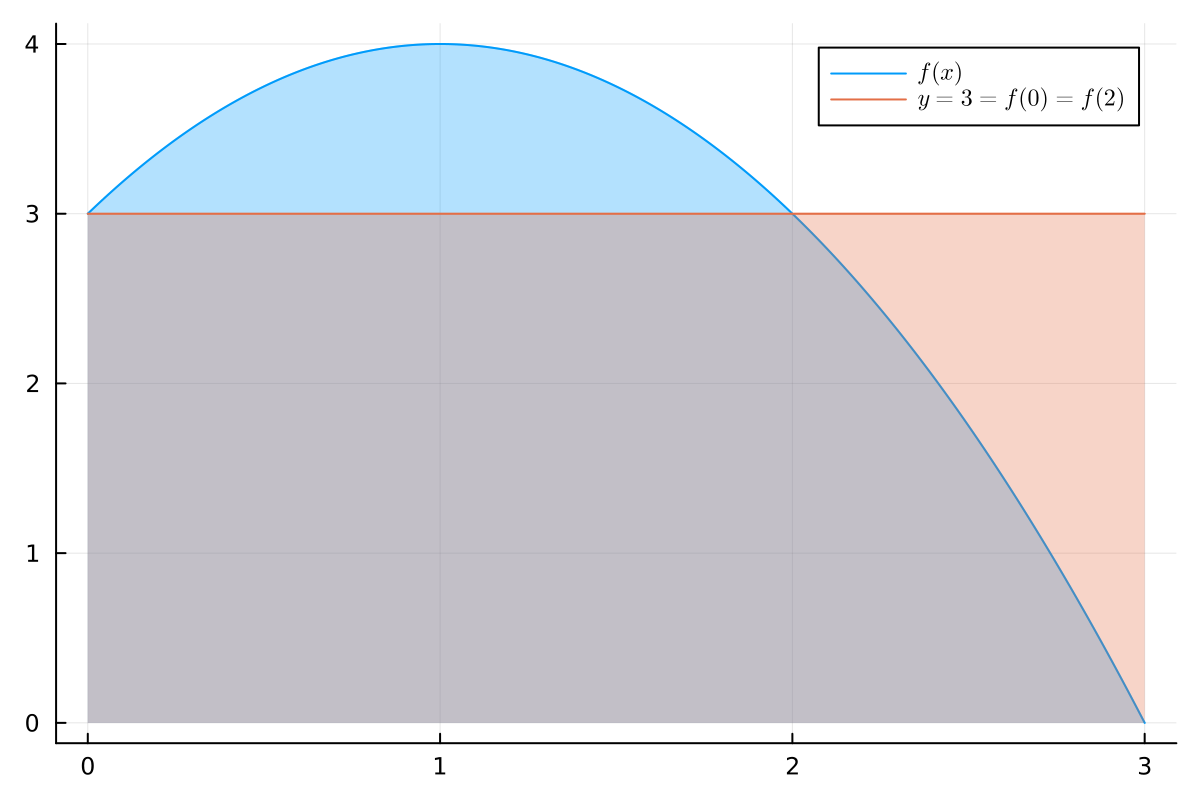
\includegraphics[width=0.7\textwidth]{figures/mean-value-theorem-for-riemann-stieltjes-integrals-first-mean-value-theorem.png}
		\caption{The area under $f$ equals the area under $y = 3$.}
		\label{fig:7}
	\end{figure}

\end{example}



\begin{theorem}[Second Mean Value Theorem for Riemann-Stieltjes Integrals] \label{thm:19}
	Assume $\alpha$ is continuous and $f$ is increasing on $[a, b]$,
	then there exists a point $x_0 \in [a, b]$ such that
	\begin{align*}
		\int_a^b f \dif \alpha
		= f(a) \int_a^{x_0} \dif \alpha + f(b) \int_{x_0}^b \dif \alpha
	\end{align*}
\end{theorem}

The second mean value theorem can be proved easily
using the first mean value theorem and integration by parts.


\begin{proof}

	Because $\alpha$ is continuous and $f$ is increasing,
	it is clear that $f \in \mathfrak{R}(\alpha)$ on $[a, b]$
	and, of course, $\alpha \in \mathfrak{R}(f)$ on $[a, b]$.

	Applying the first mean value theorem (Theorem~\ref{thm:18}),
	we have
	\begin{align}
		\int_a^b \alpha \dif f = \alpha(x_0) [f(b) - f(a)]
		\label{eq:58}
	\end{align}
	for some $x_0 \in [a, b]$.
	On the other hand, by the theorem of integration by parts, we have
	\begin{align}
		\int_a^b f \dif \alpha + \int_a^b \alpha \dif f
		= f(b) \alpha(b) - f(a) \alpha(a)
		\label{eq:59}
	\end{align}
	Combining \eqref{eq:58} and \eqref{eq:59}, we obtain that
	\begin{align*}
		\int_a^b f \dif \alpha
		 & = f(b) \alpha(b) - f(a) \alpha(a)
		- f(b) \alpha(x_0) + f(a) \alpha(x_0)                              \\
		 & = f(a)[\alpha(x_0) - \alpha(a)] + f(b)[\alpha(b) - \alpha(x_0)] \\
		 & = f(a) \int_a^{x_0} \dif \alpha + f(b) \int_{x_0}^b \dif \alpha
	\end{align*}
	which is as desired.
\end{proof}

\begin{example}
	For Riemann integrals,
	we can interpret Theorem~\ref{thm:19} as follows.
	For example, consider $f(x) = 2 - \cos(x), \; x \in [0, \pi]$.
	By the second mean value theorem, we can find a point $x_0 \in [0, \pi]$
	(in this case, $x_0 = \pi / 2$) such that
	the area under $f$ is equal to the sum of areas of two rectangles.
	One rectangle has width $x_0 - a = \pi/2 - 0$ and height $f(a) = f(0)$.
	And the other one has width $b - x_0=\pi -  \pi/2$ and height $f(b) = f(\pi)$.
	See Figure~\ref{fig:8} for an illustration.

	\begin{figure}[H]
		\centering
		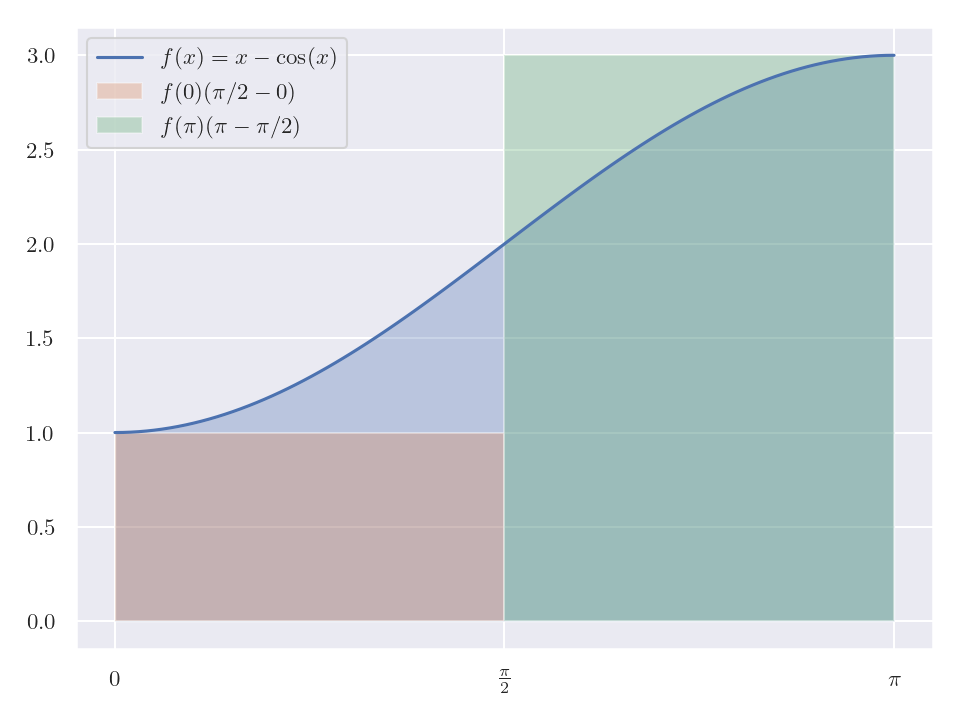
\includegraphics[width=0.7\textwidth]{figures/mean-value-theorem-for-riemann-stieltjes-integrals-second-mean-value-theorem.png}
		\caption{The area under $f$ can be decomposed of two rectangles.}
		\label{fig:8}
	\end{figure}
\end{example}



\section{The Function of Variable Upper Limit Integrals}

\begin{theorem} \label{thm:21}
	Let $\alpha$ be of bounded variation on $[a, b]$
	and $f \in \mathfrak{R}(\alpha)$ on $[a, b]$.
	Let function $F(x)$ be defined by
	\begin{align*}
		F(x) = \int_a^x f \dif \alpha, \quad x \in [a, b]
	\end{align*}
	(By Theorem~\ref{thm:13} we see that $F$ is well defined.)
	Then we have the following statements:
	\begin{enumerate}
		\item $F$ is of bounded variation on $[a, b]$.
		\item Every point of continuity of $\alpha$
		      is also a point of continuity of $F$.
		      In other words, if $\alpha$ is continuous at $x_0 \in [a, b]$,
		      then $F$ is also continuous at $x_0$.
		\item Assume further that $\alpha$ is increasing on $[a, b]$.
		      Then $F^\prime(x)$ exists at $x \in (a, b)$
		      where $\alpha^\prime(x)$ exists
		      and where $f$ is continuous.
		      For such $x$, we have
		      \begin{align*}
			      F^\prime(x) = f(x) \alpha^\prime(x)
		      \end{align*}
		      And if the left side derivative $\alpha^\prime_+(a)$ exists
		      and $f$ is continuous at the left endpoint,
		      then the left derivate of $F$ also exists.
		      An analogous statement holds for the right endpoint.
		      \begin{align*}
			      F^\prime(a)_+ = f(a) \alpha^\prime_+(a)
			      \quad \text{or} \quad
			      F^\prime(b)_{-} = f(b) \alpha^\prime_-(b)
		      \end{align*}
	\end{enumerate}
\end{theorem}

\begin{proof}
	\noindent\textbf{Proof of 1:} We will use the first mean value theorem
	and the condition that $\alpha$ is of bounded variation on $[a, b]$.

	Because $\alpha$ is of bounded variation on $[a, b]$, by definition,
	there exists $M_1 > 0$ such that
	\begin{align*}
		\sum_{k} \abs{\Delta \alpha_k} < M_1
	\end{align*}
	for all partition $P$ of $[a, b]$.

	Suppose $f$ is bounded by $M_2 > 0$.
	Let $M = M_1 M_2$.
	We will show that $\sum_{k} \abs{\Delta F_k} < M$ for all partition $P$.

	Let $P = \{x_0, \ldots, x_n\}$ be an approximate partition of $[a, b]$.
	On each subinterval $[x_{k-1}, x_k]$,
	applying the first mean value theorem, we obtain
	\begin{align*}
		\abs{\Delta F_k} = \abs{\int_{x_{k-1}}^{x_k} f \dif \alpha}
		= \abs{ c_k } \abs{ \Delta \alpha_k }
		< M_2 \abs{\Delta \alpha_k}
	\end{align*}
	where $c_k$ satisfies
	that $\inf_{x\in[x_{k-1}, x_k]} f(x) \leq c_k \leq \sup_{x\in[x_{k-1}, x_k]} f(x)$.
	Summing over $k$ yields
	\begin{align*}
		\sum_{k=1}^n \abs{\Delta F_k} < M_2 \sum_{k=1}^n \abs{\Delta \alpha_k}
		< M_2 M_1 = M
	\end{align*}
	This implies that $F$ is indeed of bounded variation on $[a, b]$.

	\noindent\textbf{Proof of 2:}
	Suppose $f$ is bounded by $M > 0$.
	Let $\varepsilon > 0$ be arbitrary.
	Suppose  $\alpha$ is continuous at $x_0 \in [a, b]$.
	Then there exists $\delta > 0$ such
	that
	\begin{align*}
		\abs{x - x_0} < \delta
		\implies \abs{\alpha(x) - \alpha(x_0)} < \frac{\varepsilon}{2M}
	\end{align*}

	Assume $0 < \abs{x - x_0} < \delta$, we have
	\begin{align*}
		\abs{F(x) - F(x_0)}
		= \abs{\int_{x_0}^x f \dif \alpha}
	\end{align*}
	By the first mean value theorem,
	there exists a number $c$ in between the infimum and supremum of $f$
	on the interval with endpoints $x_0$ and $x$ such that
	\begin{align*}
		\int_{x_0}^x f \dif \alpha = c [\alpha(x) - \alpha(x_0)]
	\end{align*}
	It then follows that
	\begin{align*}
		\abs{F(x) - F(x_0)} = \abs{c} \abs{\alpha(x) - \alpha(x_0)}
		\leq M \frac{\varepsilon}{2M} = \varepsilon / 2< \varepsilon
	\end{align*}
	This proves that $F$ is continuous at $x_0$.

	\noindent\textbf{Proof of 3:}
	For any $h \neq 0$ such that $x+h \in (a, b)$, we have
	\begin{align*}
		\frac{F(x+h) - F(x)}{h}
		= \frac{1}{h} \int_{x}^{x+h} f \dif \alpha
	\end{align*}
	By the first mean value theorem and the condition that $f$ is continuous,
	there exists $t$ in between $x$ and $x+h$
	(we have $\abs{t - x} < \abs{h}$) such that
	\begin{align*}
		\frac{1}{h} \int_{x}^{x+h} f \dif \alpha
		= f(t) \frac{\alpha(x+h) - \alpha(x)}{h}
	\end{align*}
	Because $\alpha^\prime(x)$ exists and $f$ is continuous at $x$,
	the limit of RHS of the above equation exists as $h \to 0$,
	we have
	\begin{align*}
		\lim_{h \to 0} f(t) \frac{\alpha(x+h) - \alpha(x)}{h}
		= f(x) \alpha^\prime(x)
	\end{align*}
	This completes the proof.
\end{proof}

Specially, if we assume the integrator $\alpha(x) = x$,
then we will obtain the
\textbf{first fundamental theorem of calculus}
\index{first fundamental theorem of calculus}
stated as follows.


\begin{theorem}[First Fundamental Theorem of Calculus] \label{thm:25}
	Let $F(x)$ be defined by
	\begin{align*}
		F(x) = \int_a^x f(t) \dif t, \quad
		x \in [a, b]
	\end{align*}
	Then $F$ is of bounded variation on $[a, b]$,
	and $F^\prime(x)$ exists at $x \in (a, b)$
	where $f$ is continuous.
	For such $x$, we have
	\begin{align*}
		F^\prime(x) = f(x)
	\end{align*}
	If $f$ is continuous at the endpoint $a$ or $b$,
	then the one-sided derivate of $F$ also exists there.
	In that case,
	\begin{align*}
		F^\prime_+(a) = f(a)
		\quad \text{or} \quad
		F^\prime_{-} (b) = f(b)
	\end{align*}
\end{theorem}

\begin{example}
	Consider $f(x) = \abs{x}, \; x \in [-1, 1]$
	and $F(x) = \int_{-1}^x f(t) \dif t, x \in [-1, 1]$.
	We know that $F^(x)$ exists in $(-1, 1)$
	and its one-sided derivatives exist at endpoints.
	Consider the function $\tilde{F}$ defined by
	\begin{align*}
		\tilde{F}(x)
		= \begin{cases}
			  -\frac{1}{2} x^2, & x \in [-1, 0) \\
			  \frac{1}{2} x^2,  & x \in [0, 1]
		  \end{cases}
	\end{align*}
	By calculating the derivative of $\tilde{F}$,
	we find that
	\begin{align*}
		\tilde{F}^\prime(x) = \abs{x} = f(x) \quad \forall x \in (-1, 1)
	\end{align*}
	And the one-sided derivatives $\tilde{F}^\prime_{+}(-1) = 1 = f(-1)$
	and $\tilde{F}^\prime_{-}(1) = 1 = f(1)$.
	Therefore, by Rolle's theorem, $F$ and $t\tilde{F}$ differs by a constant $c$,
	$F(x) = \tilde{F}(x) + c, \; x\in [-1, 1]$.
	Since $F(-1) = 0$, it follows that $c = \frac{1}{2}$.
	In conclusion, we have
	\begin{align*}
		F(x) = \frac{1}{2} \sgn(x) x^2 + \frac{1}{2}, \quad x \in [-1, 1]
	\end{align*}

	The graphs of $f$ and $F$ are shown in Figure~\ref{fig:9}.
	\begin{figure}[H]
		\centering
		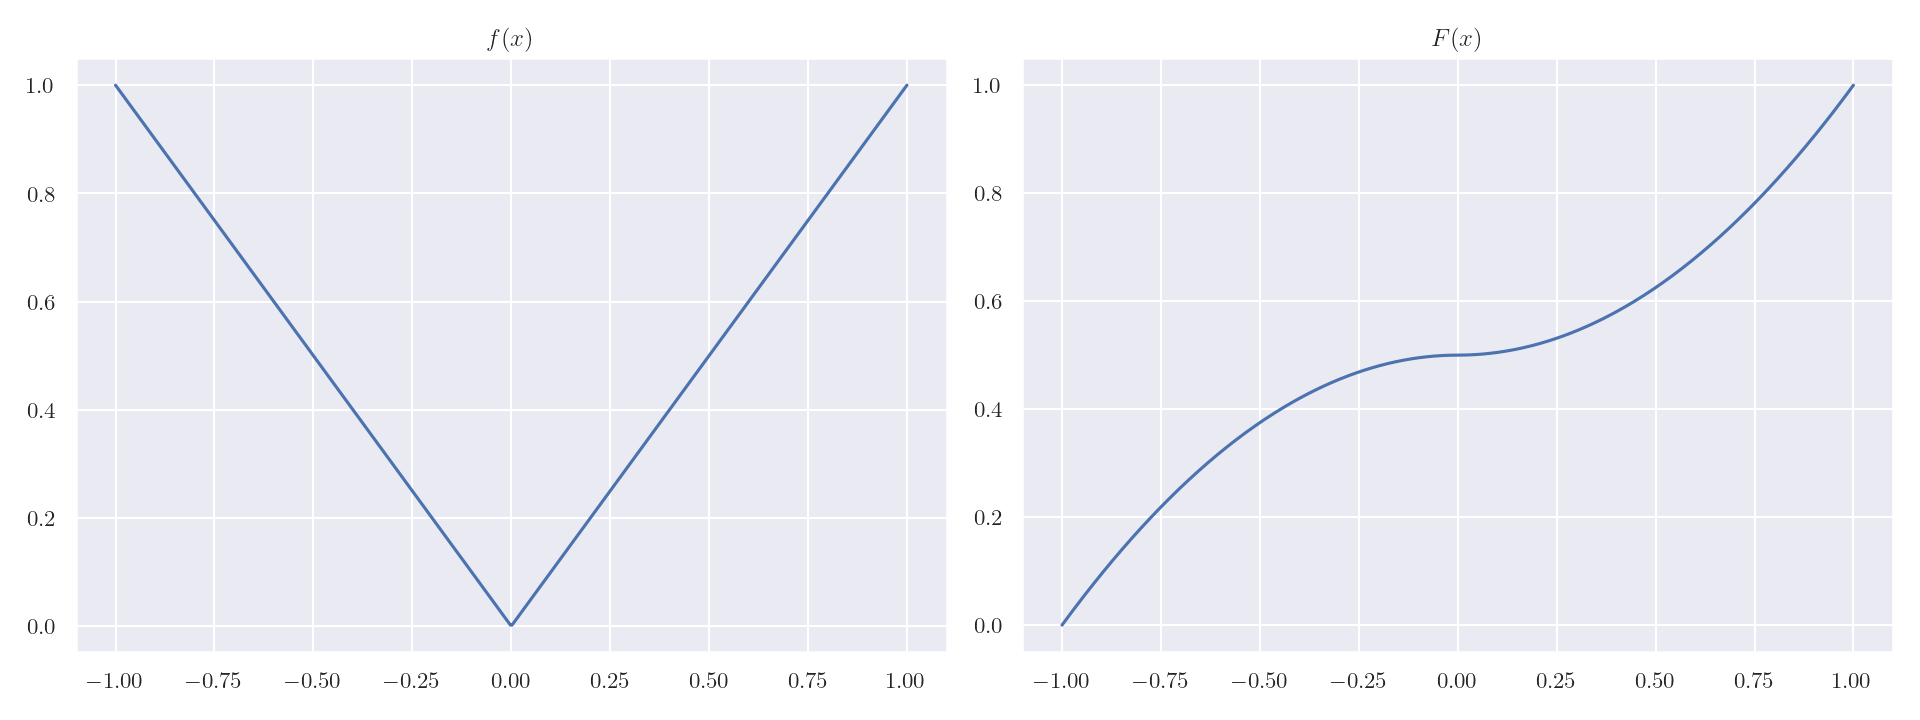
\includegraphics[width=0.7\textwidth]{figures/absolute-value-function-and-its-antiderivative.png}
		\caption{Left: function $f(x) = \abs{x}$; Right: $F(x) = \int_{-1}^x f(t) \dif t$.}
		\label{fig:9}
	\end{figure}

	Observe that the original function $f$ has a sharp turn at $x=0$.
	However, upon integration,
	the resulting function becomes smoother in the sense that it gains differentiability.
\end{example}

Combining Theorem~\ref{thm:20} and Theorem~\ref{thm:21},
we obtain the following theorem
which converts the Riemann integral of product $fg$
to a Riemann-Stieltjes integral $\int_a^b f \dif G$ or $\int_a^b g \dif F$.

\begin{theorem} \label{thm:23}
	Assume $f, g \in \mathfrak{R}$ on $[a, b]$.
	Let
	\begin{align*}
		F(x) = \int_a^x f(t) \dif t, \quad
		G(x) = \int_a^x g(t) \dif t, \quad
		x \in [a, b]
	\end{align*}
	Then $F$ and $G$ are continuous functions of bounded variation on $[a, b]$.
	Moreover, $f \in \mathfrak{R}(G)$ and $g \in \mathfrak{R}(F)$ on $[a, b]$,
	and we have
	\begin{align*}
		\int_a^b f(x) g(x) \dif x
		= \int_a^b f(x) \dif G(x)
		= \int_a^b g(x) \dif F(x)
	\end{align*}
\end{theorem}



\section{Second Fundamental Theorem of Calculus}

The first fundamental theorem of calculus
tells us about nice properties of the function
constructed from integrating a integrable function.

The following theorem, on the other hand, provides a method for evaluating the integral of a derivative.

\begin{theorem}[Second Fundamental Theorem of Calculus] \label{thm:22}
	Assume $f \in \mathfrak{R}$ on $[a, b]$.
	Let $F$ be a continuous function defined on $[a, b]$
	such that the derivative $F^\prime$ exists in $(a, b)$ and
	\begin{align*}
		F^\prime(x) = f(x) \quad \forall x \in (a, b)
	\end{align*}
	Then we have
	\begin{align*}
		\int_a^b f(x) \dif x
		= F(b) - F(a)
	\end{align*}
\end{theorem}

\begin{proof}
	Let $\varepsilon > 0$ be arbitrary.
	Since $f \in \mathfrak{R}$ on $[a, b]$,
	there exists a partition $P = \{x_0, \ldots, x_n\}$ of $[a, b]$ such that
	\begin{align*}
		\abs{S(P,T,f,x) - \int_a^b f(x) \dif x} < \varepsilon
	\end{align*}
	for any list of representatives.
	On each subinterval $[x_{k-1}, x_k]$,
	by the mean value theorem of differential calculus,
	we have
	\begin{align*}
		F(x_k) - F(x_{k-1}) = f(t_k) \Delta x_k
	\end{align*}
	where $t_k \in (x_{k-1}, x_k)$.
	Summing over $k$ yields
	\begin{align*}
		F(b) - F(a)
		= \sum_{k=1}^n f(t_k) \Delta x_k
	\end{align*}
	where the RHS is a Riemann-Stieltjes sum.
	Therefore,
	\begin{align*}
		\abs{(F(b) - F(a)) - \int_a^b f(x) \dif x} < \varepsilon
	\end{align*}
	Note that the above inequality holds for any $\varepsilon > 0$.
	This completes the proof.
\end{proof}


\begin{exercise}
	Assume further that $f$ is continuous in Theorem~\ref{thm:22}.
	Construct a simpler proof using Theorem~\ref{thm:8}.
\end{exercise}

\begin{example}
	Let
	\begin{align*}
		F(x) =\begin{cases}
			      x^2 \sin \frac{1}{x}, & x\in (0, 1] \\
			      0,                    & x=0
		      \end{cases}
	\end{align*}
	Note that $F$ is continuous on $[0, 1]$, and in the interior $(0, 1)$,
	we have
	\begin{align*}
		F^\prime(x) = 2x \sin \frac{1}{x} - \cos \frac{1}{x}
	\end{align*}
	Define $f$ on $[0, 1]$ by
	\begin{align*}
		f(x) = \begin{cases}
			       2x \sin \frac{1}{x} - \cos \frac{1}{x}, & x \in (0, 1] \\
			       0,                                      & x=0
		       \end{cases}
	\end{align*}
	Then $F^\prime(x) = f(x) \; \forall x \in (0, 1)$.
	In Example~\ref{eg:3}, we have seen that $f \in \mathfrak{R}$ on $[0, 1]$.
	Using the second fundamental theorem of calculus,
	we can evaluate the integral $\int_0^1 f(x) \dif x$:
	\begin{align*}
		\int_0^1 f(x) \dif x = F(1) - F(0) = \sin(1)
	\end{align*}
	Just for extra exercises, one may also compute that
	\begin{align*}
		\int_0^{1/\pi} f(x) \dif x = F(1/\pi) - F(0) = 0
		\quad \text{and} \quad
		\int_{1/\pi}^1 f(x) \dif x = F(1) - F(1/\pi) = \sin(1)
	\end{align*}
	A figure of $f$ and $F$ is shown in Figure~\ref{fig:10}.

	\begin{figure}[H]
		\centering
		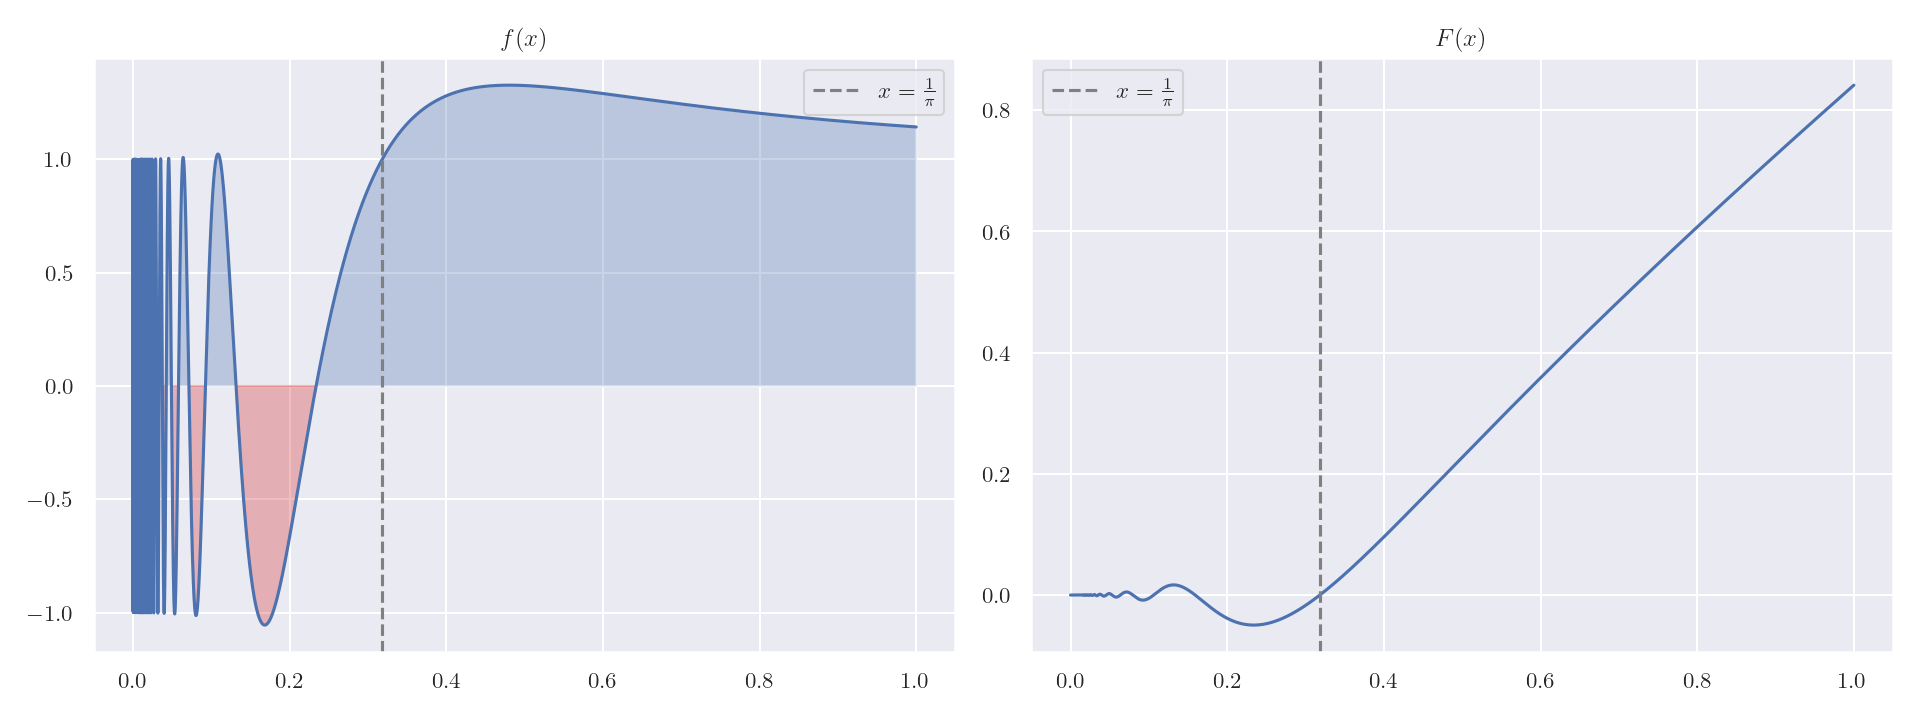
\includegraphics[width=0.9\textwidth]{figures/second-fundamental-theorem-of-calculus-example-1.png}
		\caption{Left: $f(x)$, the signed area on the left of
			the line $x=\frac{1}{\pi}$ is $0$,
			and the area on the right of the line $x=\frac{1}{\pi}$
			equalling to the overall signed area, which is $\sin(1)$;
			Right: $F(x)$, note that $F(1 / \pi) = 0$.}
		\label{fig:10}
	\end{figure}
\end{example}

The second fundamental theorem of calculus combined
with Theorem~\ref{thm:22}
can be used to strength Theorem~\ref{thm:8}.

\begin{theorem} \label{thm:27}
	Assume $f \in \mathfrak{R}$ on $[a, b]$.
	If $\alpha$ is continuous on $[a, b]$
	and its derivative $\alpha^\prime \in \mathfrak{R}$ on $[a, b]$.
	Then the following integrals exist and are equal:
	\begin{align*}
		\int_a^b f(x) \dif \alpha(x)
		= \int_a^b f(x) \alpha^\prime(x) \dif x
	\end{align*}
\end{theorem}

\begin{note}
	This theorem strengthens Theorem~\ref{thm:8}
	by relaxing the condition on $\alpha^\prime$:
	instead of requiring $\alpha^\prime$ to be continuous,
	it only requires $\alpha^\prime$ to be integrable.
\end{note}

\begin{proof}
	Let
	\begin{align*}
		A(x) = \int_a^x \alpha^\prime(t) \dif t, \quad x \in [a, b]
	\end{align*}
	By Theorem~\ref{thm:23}, we have $f \in \mathfrak{R}(A)$ on $[a, b]$,
	and
	\begin{align*}
		\int_a^b f(x) \alpha^\prime(x) \dif x
		= \int_a^b f(x) \dif A(x)
	\end{align*}
	Meanwhile, by the second fundamental theorem of calculus, we know
	\begin{align*}
		A(x) = \alpha(x) - \alpha(a)
	\end{align*}
	Due to the linearity, $f \in \mathfrak{R}(\alpha)$ and
	\begin{align*}
		\int_a^b f(x) \dif \alpha(x)
		 & = \int_a^b f(x) \dif [A(x) + \alpha(a)]                  \\
		 & = \int_a^b f(x) \dif A(x) + \int_a^b f(x) \dif \alpha(a) \\
		 & = \int_a^b f(x) \dif A(x) + 0                            \\
		 & = \int_a^b f(x) \alpha^\prime(x) \dif x
	\end{align*}
\end{proof}



\section{Change of Variables in a Riemann Integral}

\begin{theorem} \label{thm:26}
	Assume that $g$ has a continuous derivative $g^\prime$ on $[c, d]$.
	Let $f$ be continuous on $g([c, d])$
	and define $F$ by
	\begin{align*}
		F(x) = \int_{g(c)}^x f(t) \dif t,
		\quad x \in g([c, d])
	\end{align*}
	Then
	\begin{align}
		F[g(x)]
		=\int_{g(c)}^{g(x)} f(t) \dif t
		= \int_c^x f[g(t)] g^\prime(t) \dif t
		\quad \forall x \in [c, d]
		\label{eq:60}
	\end{align}
	In particular, taking $x = d$ yields
	\begin{align*}
		\int_{g(c)}^{g(d)} f(t) \dif t
		= \int_c^d f[g(t)] g^\prime(t) \dif t
	\end{align*}
\end{theorem}


\begin{note}
	Recall that a continuous function maps a connected sets to a connected sets,
	and maps compact sets to compact sets.
	Because $g$ is continuous on $[c, d]$, the image $g([c, d])$
	is actually a closed interval (when $g$ is nonconstant).
	If $g$ is constant, than $g([c, d])$ is just a single point.
\end{note}

\begin{proof}
	When $g$ is constant, the conclusion is trivial.
	In what follows, we assume $g$ is nonconstant.
	As we have noted, $g([c, d])$ is a closed interval, say $[a, b]$.
	Since $f$ is continuous on $[a, b]$,
	by the first fundamental theorem of calculus (Theorem~\ref{thm:25}),
	we have
	\begin{align*}
		F^\prime(x) = f(x) \quad \forall x \in [a, b] = g([c, d])
	\end{align*}
	For any $t \in [c, d]$, we have $g(t) \in [a, b]$.
	Substituting $x = g(t)$
	and then multiplying by $g^\prime(t)$ on both sides,
	we obtain
	\begin{align*}
		F^\prime[g(t)] g^\prime(t) = f[g(t)] g^\prime(t)
		\quad \forall t \in [c, d]
	\end{align*}
	Define function $G$ on $[c, d]$ by
	\begin{align*}
		G(t) = F[g(t)], \quad t \in [c, d]
	\end{align*}
	The chain rules implies
	\begin{align*}
		G^\prime(t)
		= F^\prime[g(t)] g^\prime(t)
		= f[g(t)] g^\prime(t)
		\quad \forall t \in [c, d]
	\end{align*}

	Note that the derivative $G^\prime(t)$ is continuous on $[c, d]$.
	Therefore, $G^\prime \in \mathfrak{R}$ on $[c, d]$
	(and hence on any subinterval, in particular, on $[c, x]$).
	Moreover, $G$ is continuous on $[c, d]$.
	Hence, we are allowed use the second fundamental theorem of calculus
	(Theorem~\ref{thm:22}) to integrate the derivate $G^\prime(t)$
	on $[c, x]$.
	We have
	\begin{align*}
		\int_c^x G^\prime(t) \dif t = G(x) - G(c)
	\end{align*}
	Plug in the formula for $H(t)$:
	\begin{align*}
		\int_c^d f^\prime[g(t)] g^\prime(t) \dif t = F[g(x)] - F[g(c)]
		= \int_{g(c)}^{g(x)} f(t) \dif t
	\end{align*}
	Note that the above equality holds for every $x \in (c, d]$,
	and it also holds when $x = c$.
\end{proof}

\begin{example}
	Consider
	\begin{align*}
		I(x) = \int_0^x \sin^2 t \cos t \dif t, \quad x \in \R
	\end{align*}
	Let $f(t) = t^2$ and $g(t) = \sin t$.
	We have
	\begin{align*}
		I(x) = \int_0^x f[g(t)] g^\prime(t) \dif t
	\end{align*}
	Apply \eqref{eq:60} in reverse direction:
	\begin{align*}
		I(x) = \int_0^x f[g(t)] g^\prime(t) \dif t
		= \int_{g(0)}^{g(x)} f(t) \dif t
		= \int_0^{\sin x} t^2 \dif t
		= \left . \frac{1}{3} t^3 \right\rvert_{0}^{\sin x}
		= \frac{1}{3} \sin^3 x
	\end{align*}

	A graph of the function $\sin^2(x) \cos(x)$ is shown in Figure~\ref{fig:11}.
	\begin{figure}[H]
		\centering
		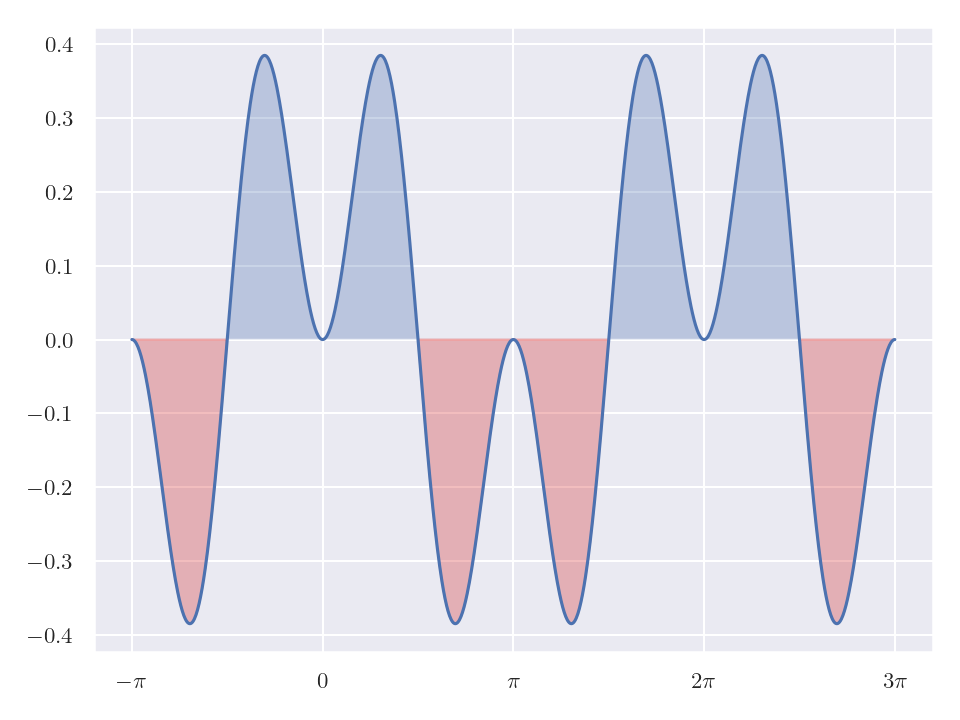
\includegraphics[width=0.7\textwidth]{figures/change-of-variables-in-a-riemann-integral-example-1.png}
		\caption{Graph of the function $\sin^2(x) \cos(x)$.}
		\label{fig:11}
	\end{figure}
\end{example}



\section{Second Mean Value Theorem for Riemann Integrals}

The second mean-value theorem provides a way of estimating the
integral of a product $f(x) g(x)$ when one function is \textit{monotonic}.

\begin{theorem}
	Let $g$ be continuous and $f$ be increasing on $[a, b]$.
	Let $A$ and $B$ be two real numbers satisfying
	\begin{align*}
		A \leq f(a+)
		\quad \text{and} \quad
		B \geq f(b-)
	\end{align*}
	Then there exists a point $x_0 \in [a, b]$ such that
	\begin{align}
		\int_a^b f(x) g(x) \dif x
		= A \int_a^{x_0} g(x) \dif x
		+ B \int_{x_0}^b g(x) \dif x
		\label{eq:61}
	\end{align}
	(Note that $f, g \in \mathfrak{R}$ on $[a, b]$, and so does their product (Theorem~\ref{thm:14}).)

	In particular, if $f(x) \geq 0$ for all $x \in [a, b]$, we have
	\begin{align}
		\int_a^b f(x) g(x) \dif x
		= B \int_{x_0}^b g(x) \dif x
		\label{eq:62}
	\end{align}
\end{theorem}

\begin{proof}
	\noindent\textbf{Proof of \eqref{eq:61}:}
	We first define a function $\tilde{f}$ on $[a, b]$ as follows:
	\begin{align*}
		\tilde{f}(x) = \begin{cases}
			               f(x), & x \in (a, b) \\
			               A,    & x=a          \\
			               B,    & x=b
		               \end{cases}
	\end{align*}
	With the given properties of $A$ and $B$, we note
	that $\tilde{f}$ is also increasing on $[a, b]$.
	And since $\tilde{f} g$ differs $f g$ by two points,
	the integrals are equal:
	\begin{align}
		\int_a^b \tilde{f}(x) g(x) \dif x
		= \int_a^b f(x) g(x) \dif x
		\label{eq:65}
	\end{align}

	Let
	\begin{align*}
		G(x) = \int_a^x g(t) \dif t, \quad x \in [a, b]
	\end{align*}
	By Theorem~\ref{thm:21}, we have $G^\prime(x) = g(x) \; \forall x \in [a, b]$.
	Then applying Theorem~\ref{thm:27}, we have
	\begin{align}
		\int_a^b \tilde{f}(x) g(x) \dif x
		= \int_a^b \tilde{f}(x) \dif G(x)
		\label{eq:64}
	\end{align}

	Next, by the second mean value theorem for Riemann-Stieltjes integrals
	(Theorem~\ref{thm:19}), there exists $x_0 \in [a, b]$ such that
	\begin{align*}
		\int_a^b \tilde{f}(x) \dif G(x)
		 & = \tilde{f}(a) \int_a^{x_0} \dif G(x)
		+ \tilde{f}(b) \int_{x_0}^b \dif G(x)    \\
		 & =  A \int_a^{x_0} \dif G(x)
		+ B \int_{x_0}^b \dif G(x)
	\end{align*}
	Apply Theorem~\ref{thm:27} again to replace $\dif G(x)$ with $g(x) \dif x$:
	\begin{align}
		\int_a^b \tilde{f}(x) \dif G(x)
		=  A \int_a^{x_0} g(x) \dif x
		+ B \int_{x_0}^b g(x) \dif x
		\label{eq:63}
	\end{align}

	Finally, combining \eqref{eq:65}, \eqref{eq:64} and \eqref{eq:63} together,
	we obtain
	\begin{align*}
		\int_a^b f(x) g(x) \dif x
		=  A \int_a^{x_0} g(x) \dif x
		+ B \int_{x_0}^b g(x) \dif x
	\end{align*}



	\noindent\textbf{Proof of \eqref{eq:62}:}
	Let $A = 0$ and $B \geq f(b-)$.
	Since $f$ is assumed to be nonnegative on $[a, b]$,
	it holds that $A \leq f(a+)$, and hence \eqref{eq:61} is applicable.
	We have
	\begin{align*}
		\int_a^b f(x) g(x) \dif x
		=  A \int_a^{x_0} g(x) \dif x
		+ B \int_{x_0}^b g(x) \dif x
		=  B \int_{x_0}^b g(x) \dif x
	\end{align*}
	for some $x_0 \in [a, b]$.

\end{proof}

An analogous result holds when $f$ is decreasing on $[a, b]$.
In that case, if $A \geq f(a+)$ and $B \leq f(b-)$, then
there exists $x_0 \in [a, b]$ such that
\begin{align*}
	\int_a^b f(x) g(x) \dif x
	= A \int_a^{x_0} g(x) \dif x
	+ B \int_{x_0}^b g(x) \dif x
\end{align*}
In particular, if $f$ is nonpositive, then
\begin{align*}
	\int_a^b f(x) g(x) \dif x
	= A \int_a^{x_0} g(x) \dif x
\end{align*}

\begin{exercise}
	Show that
	\begin{align*}
		\abs{\int_a^b \frac{\sin x}{x} \dif x} \leq \frac{2}{a}
	\end{align*}
	where $0 < a < b$.
\end{exercise}

\begin{proof}
	Let $f(x) = \frac{1}{x}$ and $g(x) = \sin x$.
	Note that $f$ is decreasing and nonnegative on $[a, b]$,
	and $g$ is continuous on $[a, b]$.
	The second mean-value theorem implies that
	\begin{align*}
		\int_a^b \frac{\sin x}{x} \dif x
		= \frac{1}{a} \int_a^{x_0} \sin x \dif x
	\end{align*}
	for some $x_0 \in [a, b]$.
	A few steps of calculation yield
	\begin{align*}
		\frac{1}{a} \int_a^{x_0} \sin x \dif x
		 & = \frac{1}{a} \left . (-\cos x) \right\rvert_{a}^{x_0} \\
		 & = \frac{1}{a} (\cos a - \cos x_0)
	\end{align*}
	Finally, the proof is concluded by noting that $\abs{\cos a - \cos x} \leq 2$.
\end{proof}



%------------------------------

\section{Riemann Stieltjes Integrals Depending on a Parameter}

\begin{theorem} \label{thm:29}
	Let function $f$ be continuous at each point $(x, y)$
	in the rectangle $[a, b] \times [c, d]$.
	Assume $\alpha$ is of bounded variation on $[a, b]$.
	Define $F$ on $[c, d]$ by
	\begin{align*}
		F(y) = \int_a^b f(x, y) \dif \alpha(x), \quad y \in [c, d]
	\end{align*}
	(Note that $F(y)$ is well-defined since  $\alpha$ is of bounded on $[a, b]$
	and for a fixed $y$, $f(x, y)$
	can be regarded as a continuous function of $x$ on $[a, b]$.)

	We have that $F$ is continuous on $[c, d]$.
	In other words, we may change the order of limit and integration, i.e.,
	for each $y_0 \in [c, d]$, we have
	\begin{align*}
		\lim_{y \to y_0} \int_a^b f(x, y) \dif \alpha(x)
		= \int_a^b \lim_{y \to y_0} f(x, y) \dif \alpha(x)
		= \int_a^b f(x, y_0) \dif \alpha(x)
	\end{align*}
\end{theorem}

\begin{proof}
	It suffices to prove this theorem assuming that $\alpha$ is increasing.
	If $\alpha$ is constant, then the conclusion is trivial.
	Hence, in the following we also assume $\alpha$ is nonconstant.

	Let $\varepsilon > 0$ be arbitrary.
	Because $f$ is continuous uniformly on $[a, b] \times [c, d]$
	(since $[a, b] \times [c, d]$ is compact),
	there exists $\delta > 0$ such that
	\begin{align*}
		\norm{(x_1, y_1) - (x_2, y_2)} < \delta
		\implies \abs{f(x_1, y_1) - f(x_2, y_2)}
		< \frac{\varepsilon}{\alpha(b) - \alpha(a)}
	\end{align*}
	for each pair of points $(x_1, y_1)$ and $(x_2, y_2)$ in the rectangle.
	In particular, consider the pair of points $(x, y)$ and $(x, y_0)$.
	We have
	\begin{align*}
		\norm{(x, y) - (x, y_0)} = \abs{y - y_0} < \delta
		\implies \abs{f(x, y) - f(x, y_0)}
		< \frac{\varepsilon}{\alpha(b) - \alpha(a)}
	\end{align*}

	Let $y$ satisfy that $\abs{y - y_0} < \delta$.
	It then follows from the comparison theorem (Theorem~\ref{thm:28}) that
	\begin{align*}
		\abs{F(y) - F(y_0)}
		 & = \abs{\int_a^b [f(x, y) - f(x, y_0)] \dif \alpha(x)}               \\
		 & \leq \int_a^b \abs{f(x, y) - f(x, y_0)} \dif \alpha(x)              \\
		 & < \int_a^b \frac{\varepsilon}{\alpha(b) - \alpha(a)} \dif \alpha(x) \\
		 & = \varepsilon
	\end{align*}
	This completes the proof.
\end{proof}

By converting $g(x) \dif x$ to $\dif G(x)$,
we may obtain a version of the above theorem for Riemann integrals.

\begin{theorem}
	Let function $f$ be continuous at each point $(x, y)$
	in the rectangle $[a, b] \times [c, d]$.
	Assume $g$ is continuous on $[a, b]$.
	Define $F$ on $[c, d]$ by
	\begin{align*}
		F(y) = \int_a^b f(x, y) g(x) \dif x, \quad y \in [c, d]
	\end{align*}
	We have that $F$ is continuous on $[c, d]$.
	In other words, we may change the order of limit and integration, i.e.,
	for each $y_0 \in [c, d]$, we have
	\begin{align*}
		\lim_{y \to y_0} \int_a^b f(x, y) g(x) \dif x
		= \int_a^b \lim_{y \to y_0} f(x, y_0) g(x) \dif x
		= \int_a^b f(x, y_0) g(x) \dif x
	\end{align*}
\end{theorem}

\begin{proof}
	For each fixed $y$, $f(x, y) \in \mathfrak{R}$ on $[a, b]$
	since it is continuous.
	Because $g$ is also Riemann integrable on $[a, b]$,
	Theorem~\ref{thm:23} is applicable.
	We may use it to convert $\int_a^b f(x, y) g(x) \dif x$
	to a Riemann-Stieltjes integral.
	Define
	\begin{align*}
		G(x) = \int_a^x g(t) \dif t, \quad x \in [a, b]
	\end{align*}
	We have
	\begin{align*}
		\int_a^b f(x, y) g(x) \dif x
		=  \int_a^b f(x, y) \dif G(x)
	\end{align*}
	Since $f$ is continuous on $[a, b]\times [c, d]$
	and $G$ is of bounded variation on $[a, b]$ (Theorem~\ref{thm:21}),
	it follows from Theorem~\ref{thm:29} that
	\begin{align*}
		\lim_{y \to y_0} \int_a^b f(x, y) \dif G(x)
		= \int_a^b lim_{y \to y_0} f(x, y) \dif G(x)
		= \int_a^b f(x, y_0) \dif G(x)
	\end{align*}
	Apply Theorem~\ref{thm:23} again to
	convert to the Riemann integral:
	\begin{align*}
		\int_a^b f(x, y_0) \dif G(x)
		= \int_a^b f(x, y_0) g(x) \dif x
	\end{align*}
	This completes the proof.
\end{proof}


%------------------------------

\section{Differentiation Under the Integral Sign}

\begin{theorem} \label{thm:30}
	Let $R = [a, b] \times [c, d]$.
	Assume that $\alpha$ is of bounded variation on $[a, b]$.
	For each point $y \in [c, d]$, assume that the integral
	\begin{align*}
		F(y) = \int_a^b f(x, y) \dif \alpha(x)
	\end{align*}
	exists.
	If the partial derivative $f_y(x, y)$ is continuous on $R$,
	then the derivative $F^\prime(y)$ exists and
	\begin{align*}
		F^\prime(y) = \int_a^b f_y(x, y) \dif \alpha(x)
		\quad \forall y \in [c, d]
	\end{align*}
\end{theorem}

To prove the existence of the derivative $F^\prime(y_0)$,
we consider the quotient
\begin{align*}
	\frac{F(y) - F(y_0)}{y - y_0}
	= \int_a^b \frac{f(x, y) - f(x, y_0)}{y - y_0} \dif \alpha(x)
\end{align*}
When taking the limit $y \to y_0$, we would like to move the
limit under the integration sign
\begin{align*}
	\lim_{y \to y_0} \int_a^b \frac{f(x, y) - f(x, y_0)}{y - y_0} \dif \alpha(x)
	= \int_a^b \lim_{y \to y_0} \frac{f(x, y) - f(x, y_0)}{y - y_0} \dif \alpha(x)
	=  \int_a^b f_y(x, y_0) \dif \alpha(x)
\end{align*}
by applying Theorem~\ref{thm:29}.
But it is valid to apply that theorem only if
we can show that $\frac{f(x, y) - f(x, y_0)}{y - y_0}$ is continuous on $R$,
which is not that easy.
We will do this by first proving the following lemma.


\begin{lemma} \label{lem:2}
	Let function $f$ be defined on a rectangle $R = [a, b] \times [c, d]$.
	If the partial derivative $f_y$, exists
	and is continuous on $R$,
	then the function
	\begin{align*}
		g(x, y) = f(x, y) - f(x, y_0), \quad (x, y) \in R
	\end{align*}
	($y_0 \in R$ is fixed) is continuous on $R$.
\end{lemma}

\begin{proof}
	Suppose $f_y$ is bounded by $M > 0$ on $R$.
	(This is possible since $f_y$ is continuous and $R$ is compact.)
	Let $\varepsilon > 0$ be arbitrary.
	Because $f_y$ is continuous uniformly on $R$,
	there exists $\delta > 0$ satisfying
	\begin{align*}
		\delta < \frac{\varepsilon / 2}{M}
	\end{align*}
	such that
	\begin{align*}
		\norm{(x_1, y_1) - (x_2, y_2)} < \delta
		\implies \abs{f(x_1, y_1) - f(x_2, y_2)} < \frac{\varepsilon / 2}{d - c}
	\end{align*}

	Choose an arbitrary point $(x, y) \in R$.
	Let numbers $h$ and $k$ be such
	that $\sqrt{h^2 + k^2} < \delta$ and $(x+h, y+k) \in R$.
	Consider the difference
	\begin{align*}
		g(x+h, y+k) - g(x, y)
		= [f(x+h, y+k) - f(x+h, y_0)] - [f(x, y) - f(x, y_0)]
	\end{align*}
	Applying the second fundamental theorem of calculus (Theorem~\ref{thm:22}),
	we have
	\begin{align}
		[f(x+h, y+k) - f(x+h, y_0)] - [f(x, y) - f(x, y_0)]
		 & = \int_{y_0}^{y+k} f_y(x+h, t) \dif t
		+ \int_{y_0}^{y} f_y(x, t) \dif t
		\label{eq:67}
	\end{align}
	Note that the mean value theorem is applicable since
	the functions $f(x+h, t)$ and $f(x, t)$ can be regarded as continuous
	functions of variable $t$ with $x+h$ and $x$ fixed.
	Rearranging the terms on the RHS of \eqref{eq:67} yields
	\begin{align}
		\int_{y_0}^{y+k} f_y(x+h, t) \dif t
		+ \int_{y_0}^{y} f_y(x, t) \dif t
		= \underbrace{\int_y^{y+k} f_y(x+h, t) \dif t}_{\text{apply the mean value theorem}}
		+ \int_{y_0}^{y} f_y(x+h, t) - f_y(x, t) \dif t
		\label{eq:68}
	\end{align}
	Because $f_y(x+h, t)$ is a continuous function of $t$,
	the mean value theorem (Theorem~\ref{thm:18}) is applicable.
	We have
	\begin{align}
		\int_y^{y+k} f_y(x+h, t) \dif t = k f_y(x+h, \bar{y})
		\label{eq:69}
	\end{align}
	for some $\bar{y}$ in between $y$ and $y+k$.
	Combining \eqref{eq:67}, \eqref{eq:68} and \eqref{eq:69}, we have
	\begin{align}
		\abs{g(x+h, y+k) - g(x, y)}
		\leq \abs{k} \abs{f_y(x+h, \bar{y})}
		+ \abs{ \int_{y_0}^y \abs{f_y(x+h, t) - f_y(x, t)} \dif t }
		\label{eq:70}
	\end{align}

	We will bound the two terms on the RHS of \eqref{eq:70} separately
	using different techniques.


	Recall $\abs{k} < \delta < \frac{\varepsilon / 2}{M}$
	and $\abs{f_y(x, y)} \leq M$.
	We have
	\begin{align}
		\abs{k} \abs{f_y(x+h, \bar{y})}
		< \frac{\varepsilon / 2}{M} \cdot M = \varepsilon / 2
		\label{eq:71}
	\end{align}

	On the other hand, since
	\begin{align*}
		\norm{(x+h, t) - (x, t)} = \abs{h} < \delta
	\end{align*}
	we have
	\begin{align*}
		\abs{f(x+h, t) - f(x, t)} < \frac{\varepsilon / 2}{d - c}
	\end{align*}
	It then follows that
	\begin{align}
		\abs{ \int_{y_0}^y \abs{f_y(x+h, t) - f_y(x, t)} \dif t }
		 & \leq \abs{ \int_{y_0}^y \frac{\varepsilon / 2}{d - c} \dif t } \nonumber \\
		 & = \frac{\varepsilon / 2}{d - c} \cdot \abs{y - y_0}       \nonumber      \\
		 & \leq \varepsilon / 2
		\label{eq:72}
	\end{align}

	Finally, it follows from \eqref{eq:70}, \eqref{eq:71} and \eqref{eq:72}
	that $\abs{g(x+h, y+k) - g(x, y)} < \varepsilon$,
	which shows that $g$ is continuous at point $(x, y)$, and hence on $R$.
\end{proof}

Now, we provide the proof of Theorem~\ref{thm:30}.

\begin{proof}
	We have
	\begin{align*}
		\int_a^b f_y(x, y_0) \dif \alpha(x)
		= \int_a^b \lim_{y \to y_0} \frac{f(x, y) - f(x, y_0)}{y - y_0} \dif \alpha(x)
	\end{align*}
	By Lemma~\ref{lem:2}, the function $f(x, y) - f(x, y_0)$ is continuous on $R$,
	so does the quotient $\frac{f(x, y) - f(x, y_0)}{y - y_0}$.
	Therefore, Theorem~\ref{thm:29} is applicable.
	We may then interchange the limit and integration:
	\begin{align*}
		\int_a^b \lim_{y \to y_0} \frac{f(x, y) - f(x, y_0)}{y - y_0} \dif \alpha(x)
		=  \lim_{y \to y_0} \int_a^b \frac{f(x, y) - f(x, y_0)}{y - y_0} \dif \alpha(x)
		=  \lim_{y \to y_0} \frac{F(y) - F(y_0)}{y - y_0}
	\end{align*}
	Therefore, the derivative $F^\prime(y_0)$ exists,
	and it equals to $\int_a^b f_y(x, y_0) \dif \alpha(x)$.
\end{proof}

The problem of the above proof is that
the function
\begin{align*}
	\phi(x, y) = \frac{f(x, y) - f(x, y_0)}{y - y_0}
\end{align*}


Alternatively, without applying Theorem~\ref{thm:29} directly.
Instead, by mimicking a similar argument in the proof of  Theorem~\ref{thm:29},
we may produce the following simpler proof of Theorem~\ref{thm:30}.

\begin{proof}
	Without loss of generality, we may assume that $\alpha$ is increasing
	and nonconstant.

	We have
	\begin{align*}
		\frac{F(y) - F(y_0)}{y - y_0}
		 & = \frac{1}{y - y_0} \int_a^b [f_y(x, y) - f_y(x, y_0)] \dif \alpha(x) \\
		 & = \int_a^b \frac{f_y(x, y) - f_y(x, y_0)}{y - y_0} \dif \alpha(x)     \\
		 & = \int_a^b f_y(x, \bar{y}) \dif \alpha(x)
	\end{align*}
	where $\bar{y}$ is in between $y$ and $y_0$.
	Note that the last equality follows from the differential mean value theorem.
	Taking the difference with $\int_a^b f_y(x, y_0) \dif \alpha(x)$ yields
	\begin{align}
		\abs{\frac{F(y) - F(y_0)}{y - y_0} - \int_a^b f_y(x, y_0) \dif \alpha(x)}
		 & = \abs{\int_a^b [f_y(x, \bar{y}) - f_y(x, y_0)] \dif \alpha(x)}  \nonumber \\
		 & \leq \int_a^b \abs{f_y(x, \bar{y}) - f_y(x, y_0)} \dif \alpha(x)
		\label{eq:66}
	\end{align}

	Let $\varepsilon > 0$ be arbitrary.
	Because $f_y$ is continuous on $R$, it is continuous uniformly there.
	There exists $\delta > 0$ such that
	\begin{align*}
		\norm{(x_1, y_1) - (x_2, y_2)} < \delta
		\implies \abs{f_y(x_1, y_1) - f_y(x_2, y_2)}
		< \frac{\varepsilon}{\alpha(b) - \alpha(a)}
	\end{align*}
	Let $y$ be such that $\abs{y - y_0} < \delta$.
	It then follows that
	\begin{align*}
		\norm{(x, \bar{y}) - (x, y_0)} = \abs{\bar{y} - y_0}
		< \abs{y - y_0} < \delta
	\end{align*}
	Therefore,
	\begin{align*}
		\abs{f_y(x, \bar{y}) - f_y(x, y_0)} < \frac{\varepsilon}{\alpha(b) - \alpha(a)}
	\end{align*}

	Combined with \eqref{eq:66}, we obtain
	\begin{align*}
		\abs{\frac{F(y) - F(y_0)}{y - y_0} - \int_a^b f_y(x, y_0) \dif \alpha(x)}
		< \int_a^b \frac{\varepsilon}{\alpha(b) - \alpha(a)} \dif \alpha(x)
		= \varepsilon
	\end{align*}
	This shows that the limit of the quotient $\frac{F(y) - F(y_0)}{y - y_0}$
	exists as $y \to y_0$, i.e., $F^\prime(y_0)$ exists, and
	it equals to $\int_a^b f_y(x, y_0) \dif \alpha(x)$.
\end{proof}



%==============================

% References
\printbibliography[heading=bibintoc, title=References]

%==============================

% Print index page
\printindex

\end{document}
